%
%---Beginning of Document---
%
% Use 1). latex ctof_manual.tex, 2). dvipdfm ctof_manual
%
\documentclass[12pt]{article}
\usepackage[dvips]{color,graphics}
\usepackage{longtable}
\usepackage{hyperref}
\usepackage[pdftex]{graphicx}
\usepackage[absolute,overlay]{textpos}
\setlength{\TPHorizModule}{1mm}
\setlength{\TPVertModule}{1mm}
%
\textwidth  6.5in
\textheight 9.0in
\topmargin 0.0 in
\headheight 0.0in
\headsep 0.0in
\oddsidemargin 0in
\evensidemargin 0in
\parsep 0 in
%\parindent 0in
\pagenumbering{arabic}
%
\setcounter{secnumdepth}{5}
\setcounter{tocdepth}{5}
%
\begin{document}

\title{Central Time-of-Flight System Operations Manual}

\vskip 0.5cm

\author{D.S. Carman, Jefferson Laboratory\\[0.2ex]
{\it ctof\_manual.tex -- v1.5}}

\date \today
%
\maketitle

\begin{abstract}
This document provides an overview of the CLAS12 Central Time-of-Flight (CTOF) 
System and serves as an Operations Manual for the detector. Instructions are 
provided for shift workers related to the basic steps of operating and monitoring 
the HV system and shield compensation coil controls, monitoring the detector 
system and responding to alarms, and knowing when to contact the on-call personnel. 
More complete details are also provided for CTOF system experts regarding the 
channel mapping to the readout electronics, the cable connections and routing in 
Hall~B, higher-order high voltage system operations, operations of the Light 
Monitoring System, and detector servicing. This document also provides references 
to the available CTOF documentation and a list of personnel authorized to perform 
CTOF system repairs and to modify system settings.
\end{abstract}

\thispagestyle{empty}

\clearpage

\vfil
\eject

\tableofcontents

\vfil
\eject

\section{CTOF Overview}
\label{intro}

The Central Time-of-Flight (CTOF) system is a major component of the CLAS12 
Central Detector used to measure the flight time of charged particles emerging 
from beam-related interactions in the target. The CTOF system spans laboratory 
angles from 35$^\circ$ to 125$^\circ$ and surrounds the experimental target at a 
radial distance of 25~cm. The CTOF detector consists of 48 92-cm-long scintillation 
bars that form a hermetic barrel. The barrel is positioned inside of the 5~T 
superconducting solenoid magnet. Each counter is read out on its upstream and
downstream ends using photomultiplier tubes (PMTs) through long light guides to 
position the field-sensitive PMTs in reduced field regions. However, even in these 
positions, the PMTs reside in inhomogeneous fringe fields from the magnet at levels 
as large as 1~kG. In order for the PMTs to operate properly at their design 
specifications for gain and timing resolution, the magnetic field about the PMTs 
needs to be reduced to a level below 1~G. Hence the CTOF PMTs must be operated 
within specially designed magnetic shields with compensation coils.

The requirements for the CTOF system (shown in Fig.~\ref{ctof-layout}) include 
excellent timing resolution for particle identification and good segmentation to 
minimize counting rates. The system specifications call for an average time 
resolution for each counter along its full length of $\sigma_{TOF}$=65~ps. The 
system must also be capable of operating in a high-rate environment at the nominal 
CLAS12 luminosity of $1 \times 10^{35}$~cm$^{-2}$s$^{-1}$. A summary of the CTOF 
technical parameters is given in Table~\ref{details}. 

%%%%%%%%%%%%%%%%%%%%%%%%%%%%%%%%%%%%%%%%%%%%%%%%%%%%%%%%%%%%%%%%%%%%%%%%%%%%%%%%%%%
\begin{figure}[htbp]
\vspace{5.2cm}
\begin{picture}(50,50) 
\put(100,-80)
{\hbox{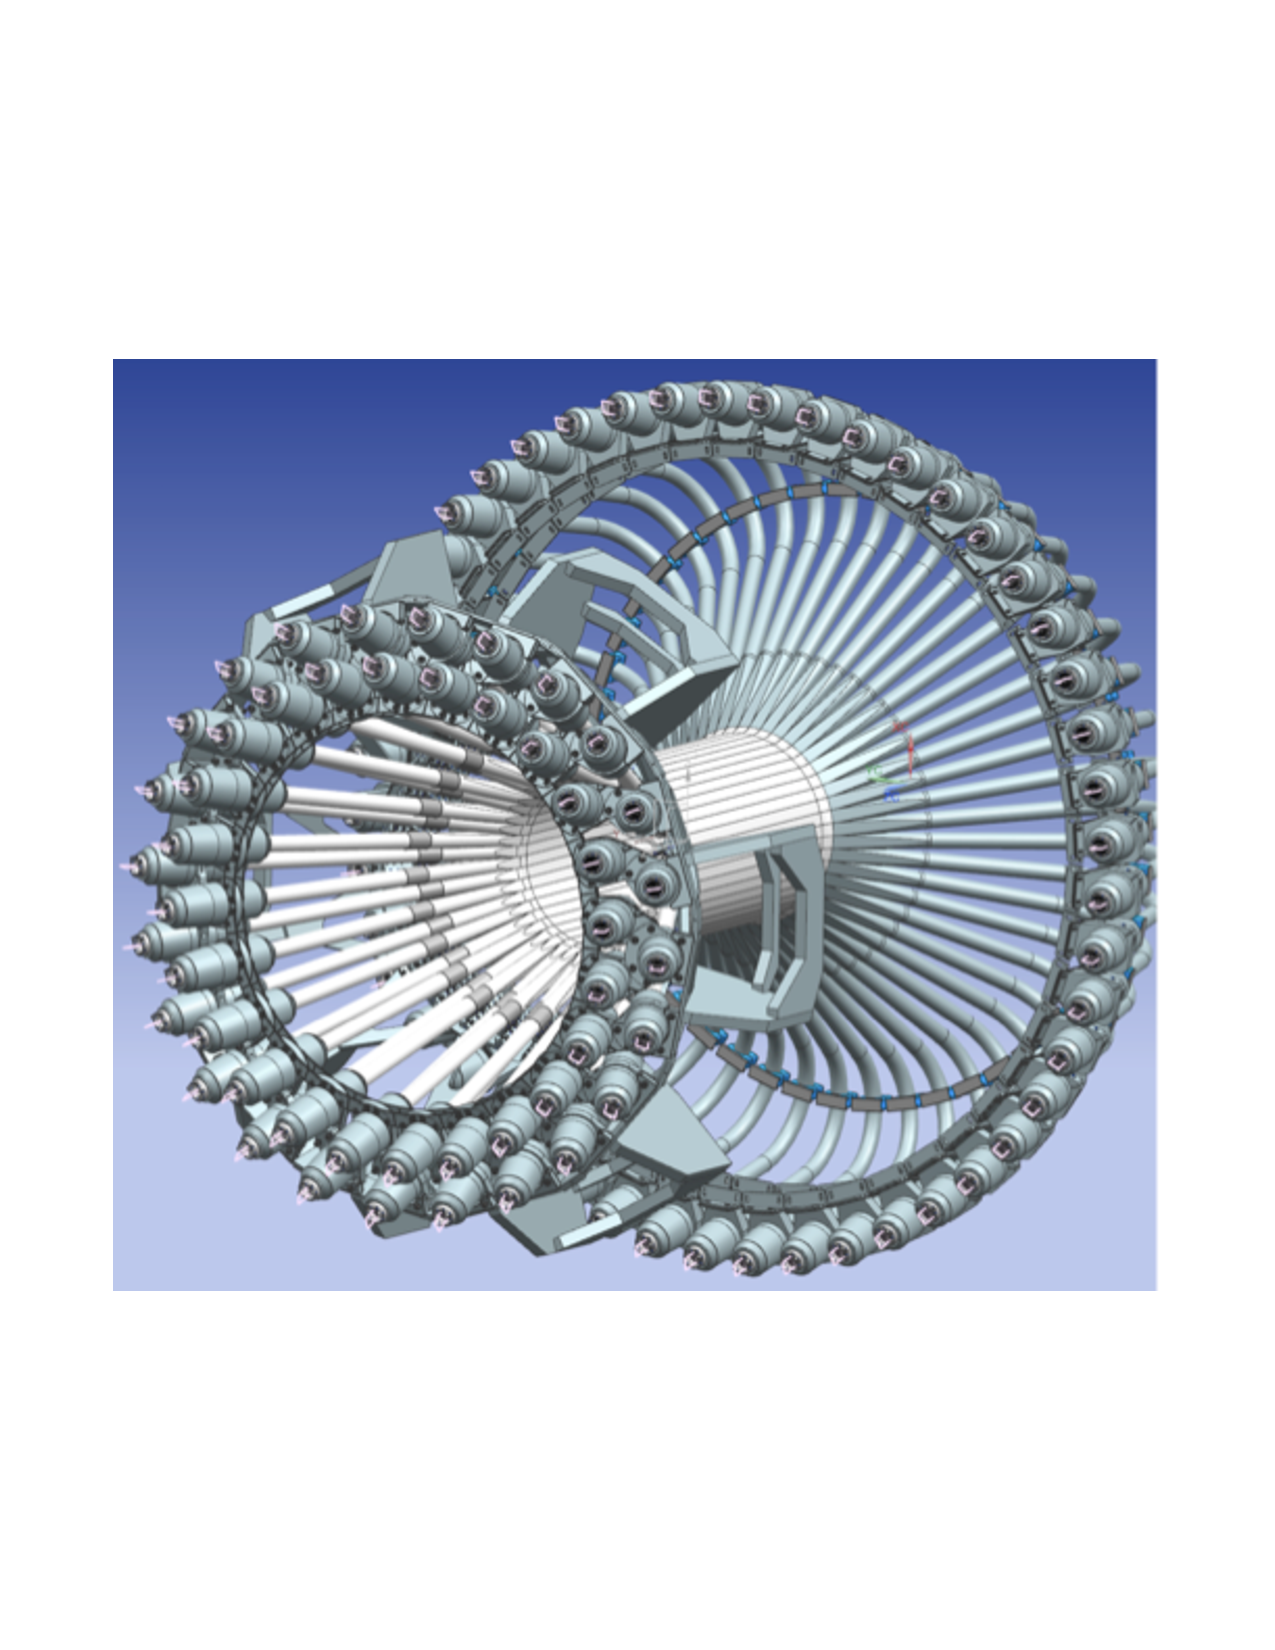
\includegraphics[width=0.58\textwidth,natwidth=610,natheight=642]{ctof.pdf}}}
\end{picture} 
\caption{View of the Central Time-of-Flight system for CLAS12 showing the upstream 
straight light guides, the scintillation bars, and the downstream bent light guides. 
The PMTs reside within the shield cylinders located at the ends of the light guides.} 
\label{ctof-layout}
\end{figure}
%%%%%%%%%%%%%%%%%%%%%%%%%%%%%%%%%%%%%%%%%%%%%%%%%%%%%%%%%%%%%%%%%%%%%%%%%%%%%%%%%%%

%%%%%%%%%%%%%%%%%%%%%%%%%%%%%%%%%%%%%%%%%%%%%%%%%%%%%%%%%%%%%%%%%%%%%%%%%%%%%%%%%%%
\begin{table}[htbp]
\begin{center}
\begin{tabular} {|l|l|} \hline
~~Parameter~~ &~~~~~~~~~~~~~~~~~~~~~~ Design Value ~~~~~~~~~~\\ \hline \hline
Counters                  & 48 BC-408 counters forming a hermetic barrel; \\
                          & double-sided readout                   \\ \hline
Angular Coverage          & $\theta$: (35$^\circ$,125$^\circ$), $\phi$: 
(-180$^\circ$,180$^\circ$) \\ \hline
Counter Dimensions        & Trapezoidal cross section $\sim 3 \times 3 \times 
92$~cm$^3$ \\ \hline
PMTs                      & Hamamatsu R2083 (H2431-MOD assembly)    \\ \hline
Light Guides - Upstream   & O.D.=$2''$, 1-m-long, focusing design, straight \\ \hline
Light Guides - Downstream & O.D.=$2''$, 1.6-m-long, focusing design, bent 135$^\circ$ \\ 
\hline
Magnetic Shields          & 3-layer cylinder: Co-netic, Hiperm-48, Steel-1008; \\ 
                          & compensation coils around inner Co-netic layer \\ \hline
Design Resolution         & 65~ps \\ \hline
$\pi$/$K$ separation      & 3.3$\sigma$ up to 0.64~GeV \\ \hline
$K$/$p$ separation        & 3.3$\sigma$ up to 1.00~GeV \\ \hline
$\pi$/$p$ separation      & 3.3$\sigma$ up to 1.25~GeV \\ \hline
\end{tabular}
\end{center}
\caption{CTOF technical design parameters.}
\label{details}
\end{table}
%%%%%%%%%%%%%%%%%%%%%%%%%%%%%%%%%%%%%%%%%%%%%%%%%%%%%%%%%%%%%%%%%%%%%%%%%%%%%%%%%%%

The CTOF scintillation barrel is composed of 48 wedge-shaped counters of two 
slightly different designs that alternate in azimuth. A pair of neighboring CTOF 
counters is shown in Fig.~\ref{counter-pair}. The difference between the two 
designs is in the pitch angle of the upstream straight light guide and the upstream 
end of the scintillation bars where they attach to this light guide. The CTOF 
detector is mounted within the CLAS12 solenoid as shown in Fig.~\ref{cut-view}. The 
beamline lies along the symmetry axis of the CTOF barrel pointing downstream (left 
to right in Fig.~\ref{cut-view}). The nominal position of the center of the CTOF
scintillation barrel is roughly 7.6~in upstream of the CLAS12 origin. 
Fig.~\ref{ctof-labeling} shows the CTOF naming convention with counter \#1 located 
at the 9 o'clock position and increasing in number going clockwise around the 
detector.

%%%%%%%%%%%%%%%%%%%%%%%%%%%%%%%%%%%%%%%%%%%%%%%%%%%%%%%%%%%%%%%%%%%%%%%%%%%%%%%%%%%
\begin{figure}[htbp]
\vspace{5.2cm}
\begin{picture}(50,50) 
\put(45,245)
{\hbox{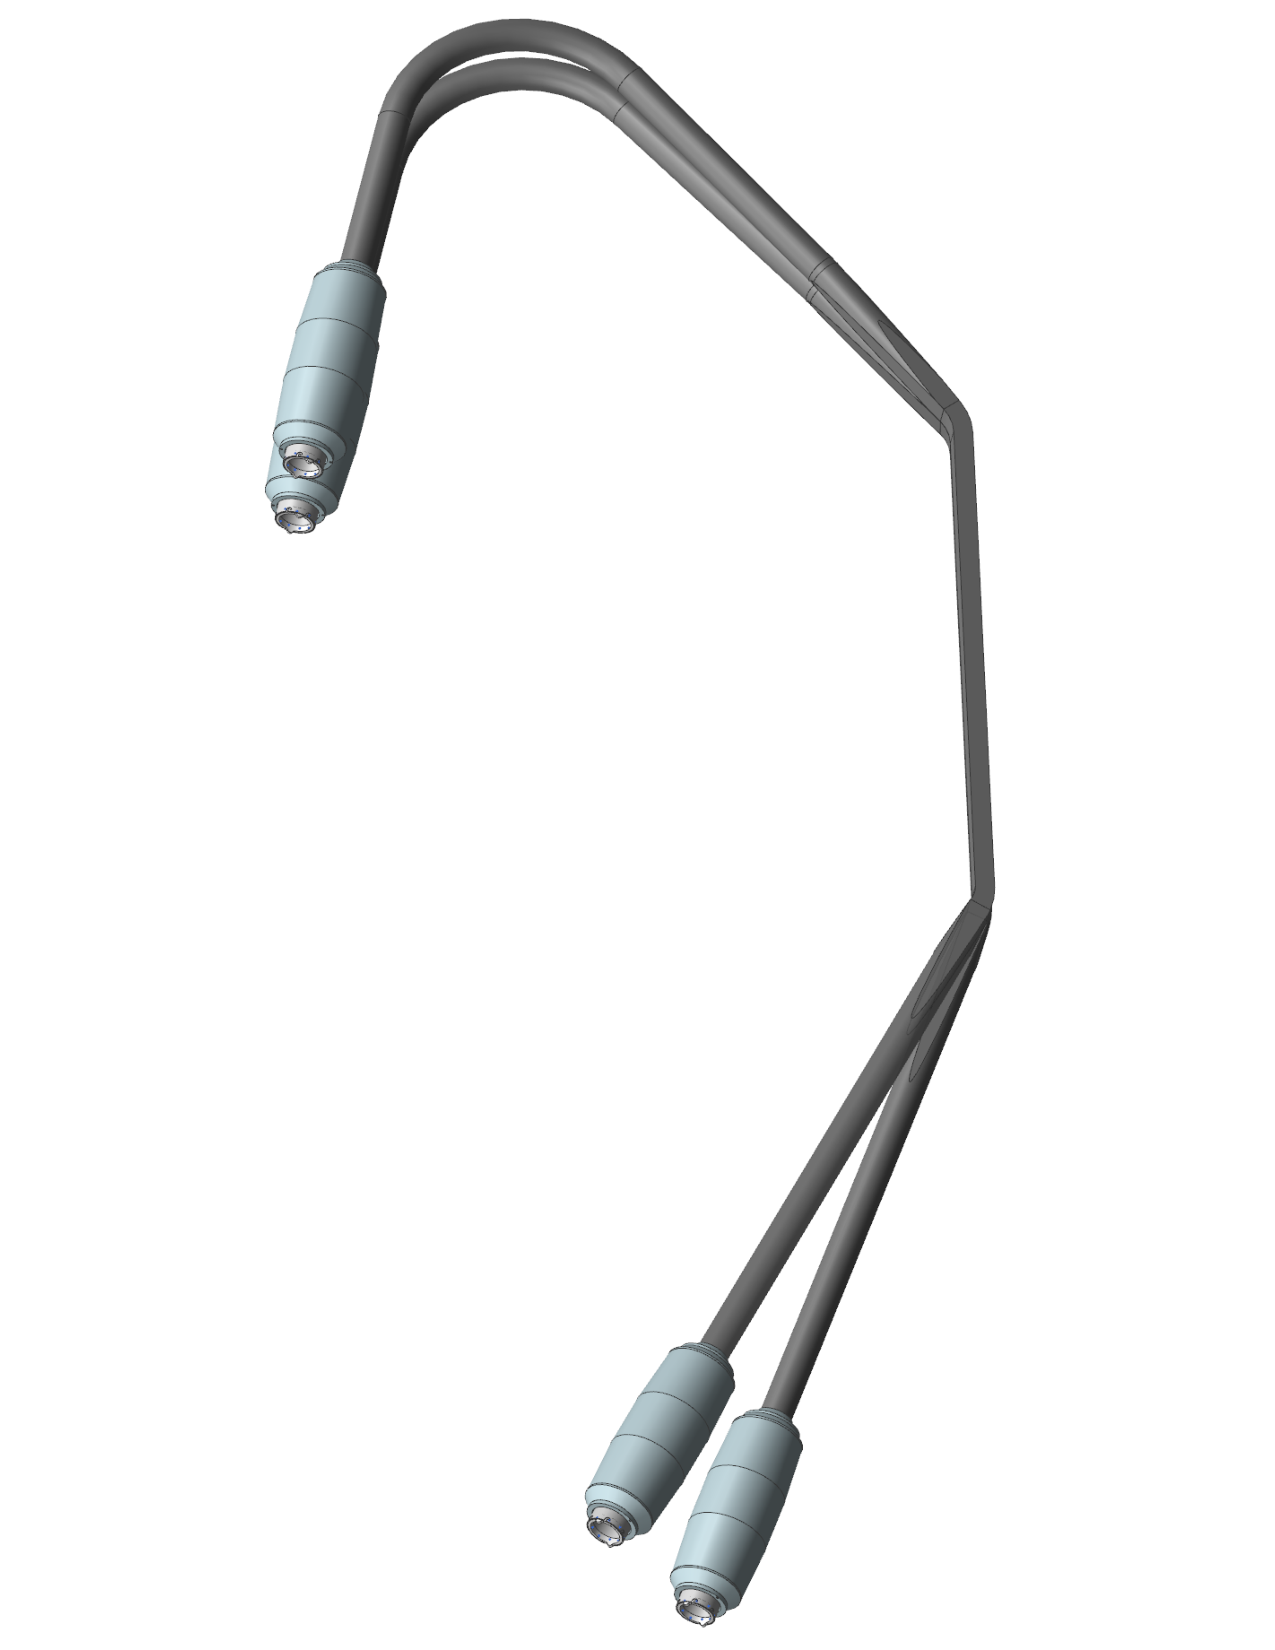
\includegraphics[width=0.62\textwidth,natwidth=610,natheight=642,angle=-90]
{counter-pair.pdf}}}
\end{picture} 
\caption{A pair of neighboring CTOF counters with two slightly different designs 
for the upstream light guide and the upstream end of the scintillation bars.} 
\label{counter-pair}
\end{figure}
%%%%%%%%%%%%%%%%%%%%%%%%%%%%%%%%%%%%%%%%%%%%%%%%%%%%%%%%%%%%%%%%%%%%%%%%%%%%%%%%%%%

%%%%%%%%%%%%%%%%%%%%%%%%%%%%%%%%%%%%%%%%%%%%%%%%%%%%%%%%%%%%%%%%%%%%%%%%%%%%%%%%%%%
\begin{figure}[htbp]
\vspace{5.6cm}
\begin{picture}(50,50) 
\put(100,5)
{\hbox{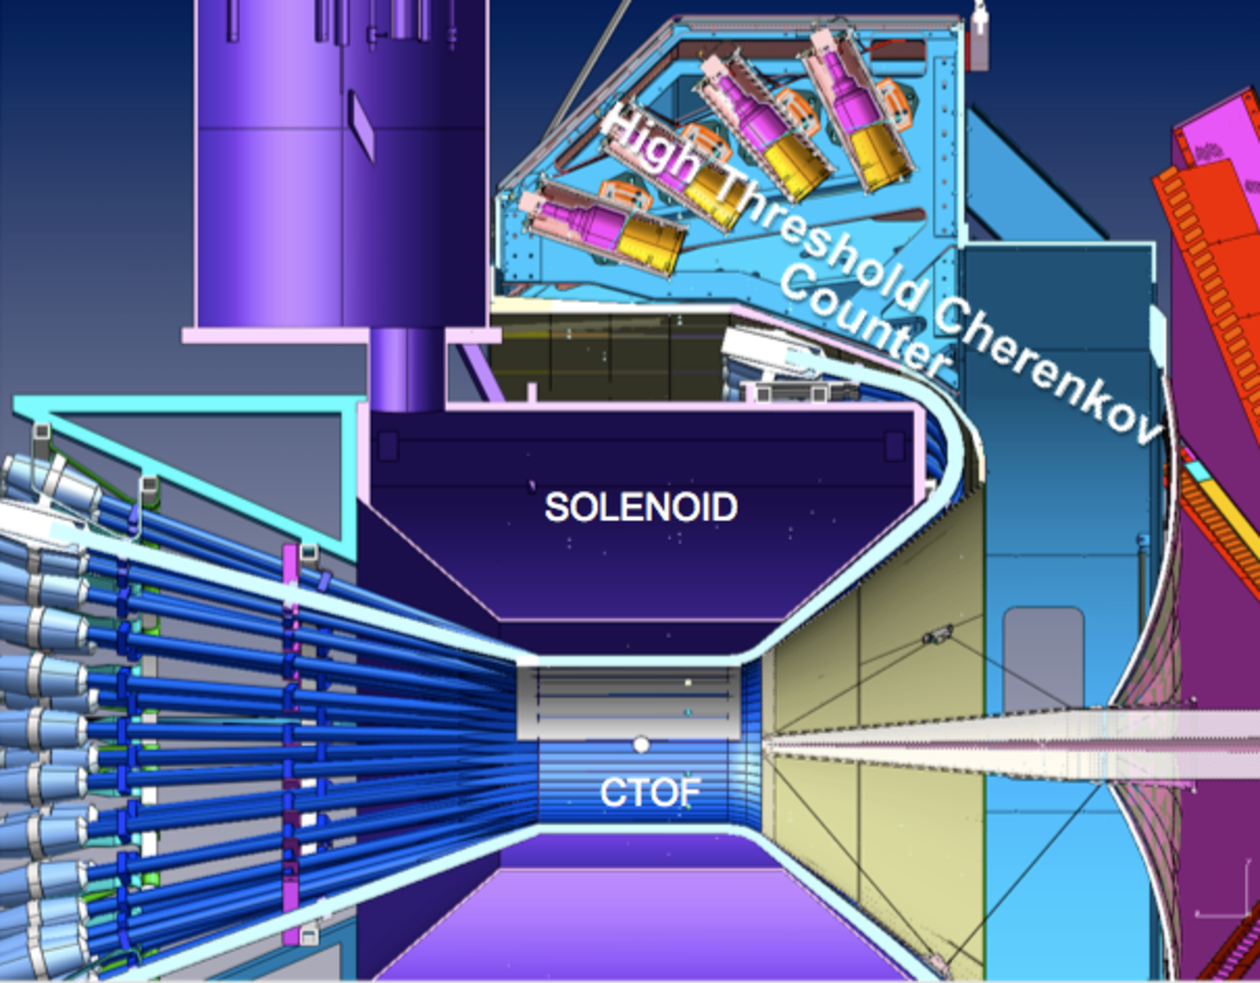
\includegraphics[width=0.58\textwidth,natwidth=610,natheight=642]
{ctof-insitu.pdf}}}
\end{picture} 
\caption{CTOF mounted within the CLAS12 solenoid in a cut view where the beam axis 
runs along the CTOF barrel symmetry axis with the beam entering from the left.}
\label{cut-view}
\end{figure}
%%%%%%%%%%%%%%%%%%%%%%%%%%%%%%%%%%%%%%%%%%%%%%%%%%%%%%%%%%%%%%%%%%%%%%%%%%%%%%%%%%%

%%%%%%%%%%%%%%%%%%%%%%%%%%%%%%%%%%%%%%%%%%%%%%%%%%%%%%%%%%%%%%%%%%%%%%%%%%%%%%%%%%%
\begin{figure}[htbp]
\vspace{5.6cm}
\begin{picture}(50,50) 
\put(130,5)
{\hbox{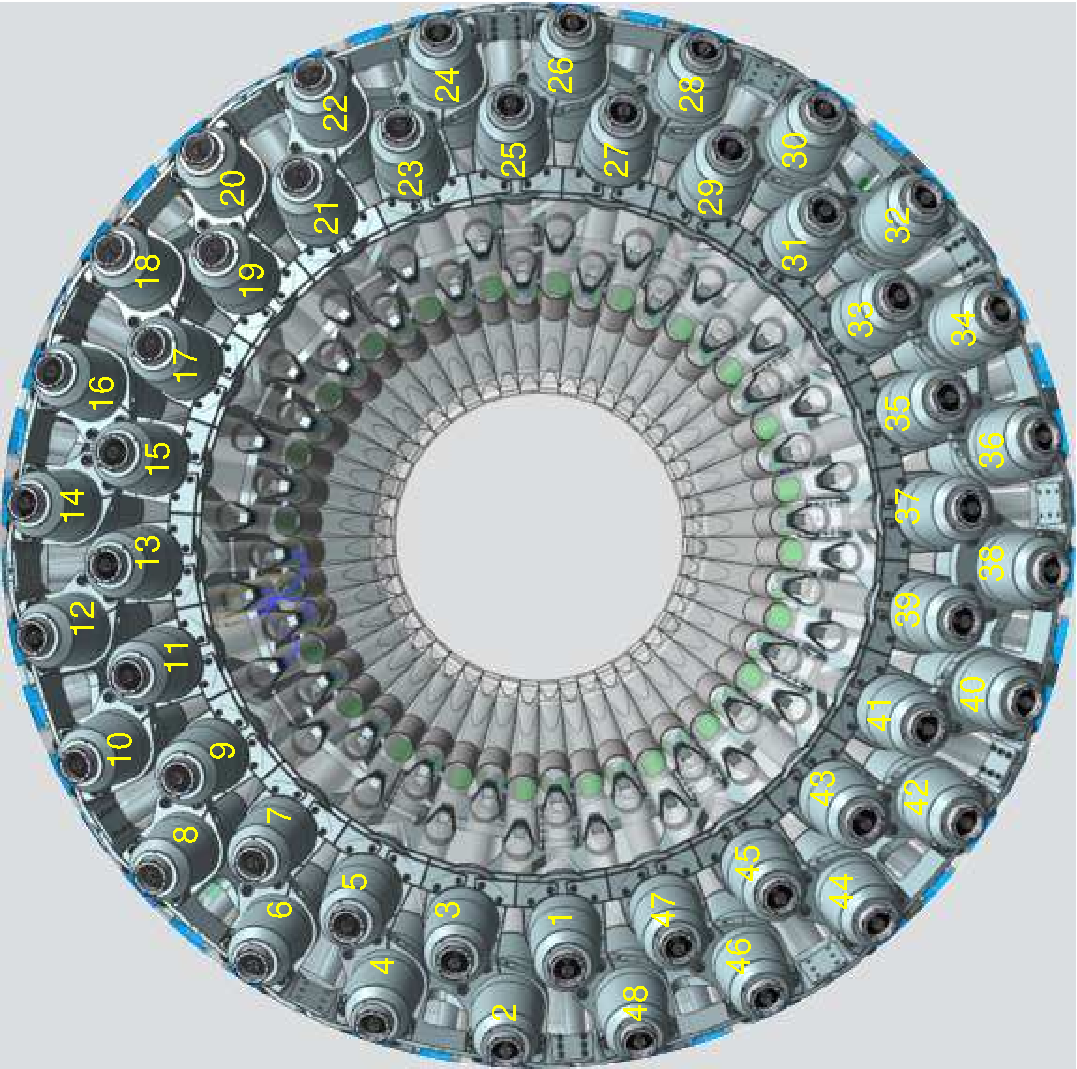
\includegraphics[width=0.58\textwidth,natwidth=610,natheight=642]
{ctof-labeling.pdf}}}
\end{picture} 
\caption{CTOF counter numbering convention seen looking at the upstream end of 
the detector.
\label{ctof-labeling}}
\end{figure}
%%%%%%%%%%%%%%%%%%%%%%%%%%%%%%%%%%%%%%%%%%%%%%%%%%%%%%%%%%%%%%%%%%%%%%%%%%%%%%%%%%%

\vfil
\eject

A block diagram of the readout electronics and power connections for one 
representative counter of the CTOF system is shown in Fig.~\ref{ctof-elec}. The 
PMT anode outputs are connected to one of two UVa 80-20 splitter boxes. The 80\% 
output goes to an Ortec 934 NIM CFD and then to a CAEN 1290A 25~ps LSB VME TDC. The 
20\% output goes to a JLab 250~MHz VME flash ADC. The high voltage (HV) power supply 
for the CTOF counters is a CAEN SY1527 mainframe outfitted with four negative polarity 
24-channel A1535N modules that is shared with the HTCC system. The CTOF HV modules
occupy slots \#0 to \#3 in the mainframe. The LV power supplies for the CTOF magnetic 
shield compensation coils are Wiener MPV8016I modules in an MPOD-mini crate. 
Fig.~\ref{elec-layout} shows the locations of the CTOF electronics and power 
supplies in the electronics racks on the beam left side of Space Frame Level~1.

%%%%%%%%%%%%%%%%%%%%%%%%%%%%%%%%%%%%%%%%%%%%%%%%%%%%%%%%%%%%%%%%%%%%%%%%%%%%%%%%%%%
\begin{figure}[htbp]
\vspace{5.8cm}
\begin{picture}(30,50) 
\put(90,10)
{\hbox{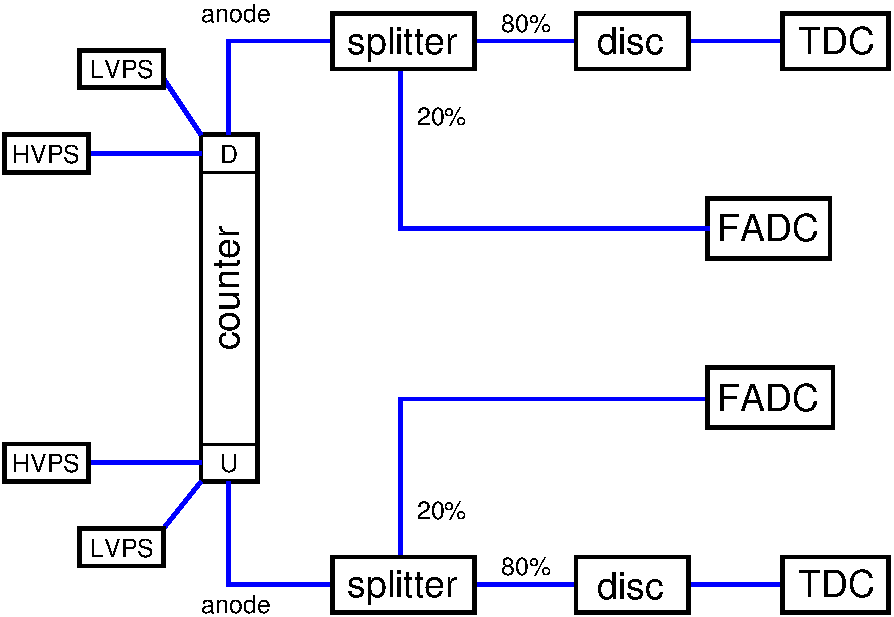
\includegraphics[width=0.85\textwidth,natwidth=610,natheight=642]
{electronics-block.pdf}}}
\end{picture} 
\caption{Block diagram for the CTOF system showing the layout of the readout 
electronics and power connections for a single counter.}
\label{ctof-elec}
\end{figure}
%%%%%%%%%%%%%%%%%%%%%%%%%%%%%%%%%%%%%%%%%%%%%%%%%%%%%%%%%%%%%%%%%%%%%%%%%%%%%%%%%%%

%%%%%%%%%%%%%%%%%%%%%%%%%%%%%%%%%%%%%%%%%%%%%%%%%%%%%%%%%%%%%%%%%%%%%%%%%%%%%%%%%%%
\begin{figure}[htbp]
\vspace{12.0cm}
\begin{picture}(30,50) 
\put(85,15)
{\hbox{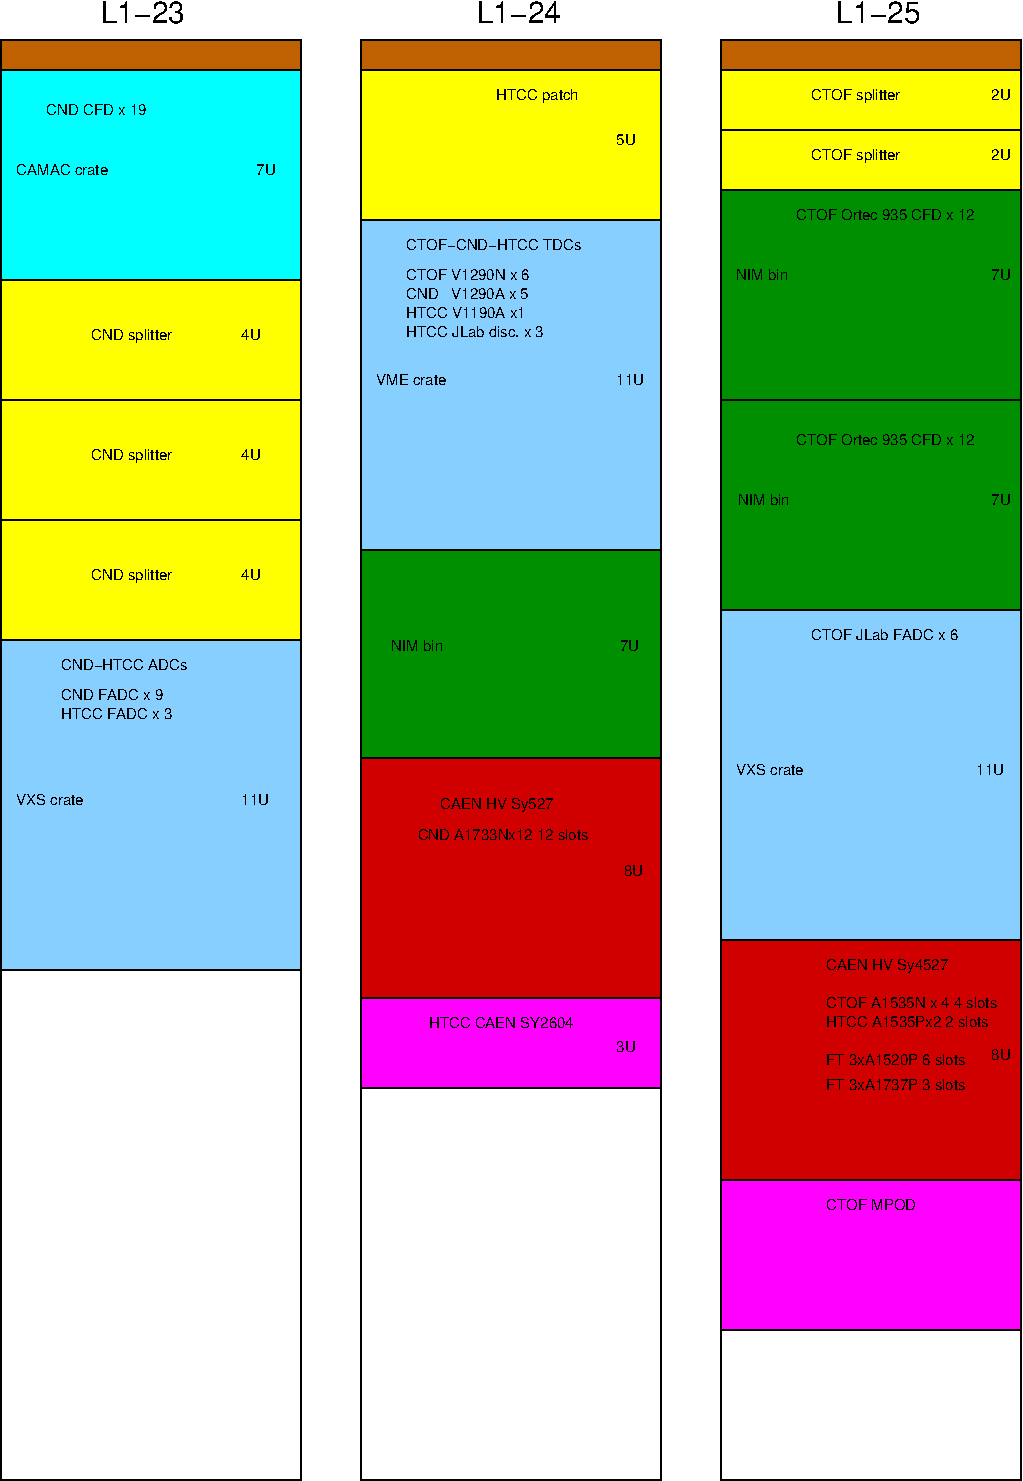
\includegraphics[width=0.80\textwidth,natwidth=610,natheight=642]
{CTOFCNDHTCC.pdf}}}
\end{picture} 
\caption{Layout of the electronics for the CTOF, CND, and HTCC NIM and VME 
electronics on the beam left side of Level~1 of the Space Frame in Hall~B. The 
positions of the HV and LV mainframes are also shown.}
\label{elec-layout}
\end{figure}
%%%%%%%%%%%%%%%%%%%%%%%%%%%%%%%%%%%%%%%%%%%%%%%%%%%%%%%%%%%%%%%%%%%%%%%%%%%%%%%%%%%

\clearpage

\vfil
\eject

\section{Information for Shift Workers}

\subsection{Shift Worker Responsibilities}

The shift worker in the Hall~B Counting House has five responsibilities with 
regard to the CTOF system:

\begin{enumerate}
\item Updating the Hall~B electronic logbook with records of problems or system 
conditions (see Section~\ref{logbook}).

\item Contacting CTOF system on-call personnel for any problems that are discovered 
(see Section~\ref{contact}).

\item Responding to CTOF system alarms from the Hall~B alarm handler (see 
Section~\ref{alarms}).

\item Turning on or off the high voltage (HV) for the CTOF system using the HV 
control interface (see Section~\ref{hv-control}).

\item Monitoring the hit occupancy scalers for the system (see Section~\ref{monitoring}).
\end{enumerate}

\subsubsection{Updating the Logbook}
\label{logbook}

The electronic logbook (or e-log)~\cite{e-log} is set up to run on a specified 
terminal in the Hall~B Counting House. Shift workers are responsible for keeping 
an up-to-date and accurate record of any problems or issues concerning the CTOF 
system. For any questions regarding the logbook, its usage, or on what is 
considered to be a ``logbook worthy'' entry, consult the assigned shift leader.

Note the shift worker should follow all posted or communicated instructions about 
entering CTOF scaler screens into the e-log. This is typically done once per 
8-hour shift as directed on the shift checklist.

\subsubsection{Contacting CTOF System Personnel}
\label{contact}

As a general rule, shift workers should spend no more than 10 to 15 minutes 
attempting to solve any problem that arises with the CTOF system. At that point 
they should contact the assigned CTOF on-call expert to provide either advice on 
how to proceed or to address the problem. \textcolor{red}{The CTOF on-call phone 
number if (757)-344-7204.}

This document is divided into sections for shift workers and for CTOF system 
experts. However, only CTOF system experts (as listed in Section~\ref{personnel}) 
are authorized to make changes to the CTOF parameter settings, to work on the 
hardware or electronics, or to modify the DAQ system software. This division 
between shift worker responsibilities and expert responsibilities is essential
to maintain in order to protect and safeguard the equipment, to ensure data 
collection is as efficient as possible, and to minimize down time. If the shift 
worker has any questions regarding how to proceed when an issue arises, the shift 
leader should be consulted.

\subsubsection{Hall~B Alarm Handler}
\label{alarms}

The BEAST alarm handler system running in the Counting House monitors the entire 
Hall~B Slow Controls system. This includes the HV and low voltage (LV) systems, 
gas systems, torus and solenoid controls, subsystem environment controls (e.g. 
temperature, humidity), and pulser calibration systems (among several others). The 
system runs on a dedicated terminal in the Counting House. One of the main 
responsibilities of the shift worker is to respond to alarms from this system, 
either by taking corrective action or by contacting the appropriate on-call personnel. 
Instructions and details on the alarm handler for Hall~B are given in Ref.~\cite{beast}.

For the CTOF system there are two elements that are monitored by the alarm handler. 
The first is the HV system. Any time a channel trips off an alarm will sound. The 
alarm handler will identify the specific channel (or channels) that have tripped. 
These channels can be reset either through the alarm handler or through the CTOF HV 
control screens. These channels should be reset only after ensuring that whatever 
condition caused the trip (e.g. bad beam conditions) has been addressed. The second 
CTOF element monitored by the alarm handler is the power status of the LV power 
supply for the magnetic shield compensation coils. An overcurrent or overtemperature 
condition at any monitored point in the system will cause the LV power supply to trip 
off. These conditions are not expected to occur during normal operation of the 
compensation coil system. If such an alarm condition occurs, the CTOF on-call expert 
should be contacted to investigate and restore the system.

\subsection{High Voltage Controls}
\label{hv-control}

The CTOF HV is controlled through the Hall~B CS-Studio suite, which is an 
Eclipse-based collection of tools used as an interface to the EPICS Slow Controls 
system. To start the user interface on any terminal in the Hall~B Counting House, 
enter the command {\it clascss}. Fig.~\ref{ctof-screen1-2}(left) shows the control 
panel that is launched.

%%%%%%%%%%%%%%%%%%%%%%%%%%%%%%%%%%%%%%%%%%%%%%%%%%%%%%%%%%%%%%%%%%%%%%%%%%%%%%%%%%%
\begin{figure}[htbp]
\vspace{8.5cm}
\begin{picture}(30,50) 
\put(50,-5)
{\hbox{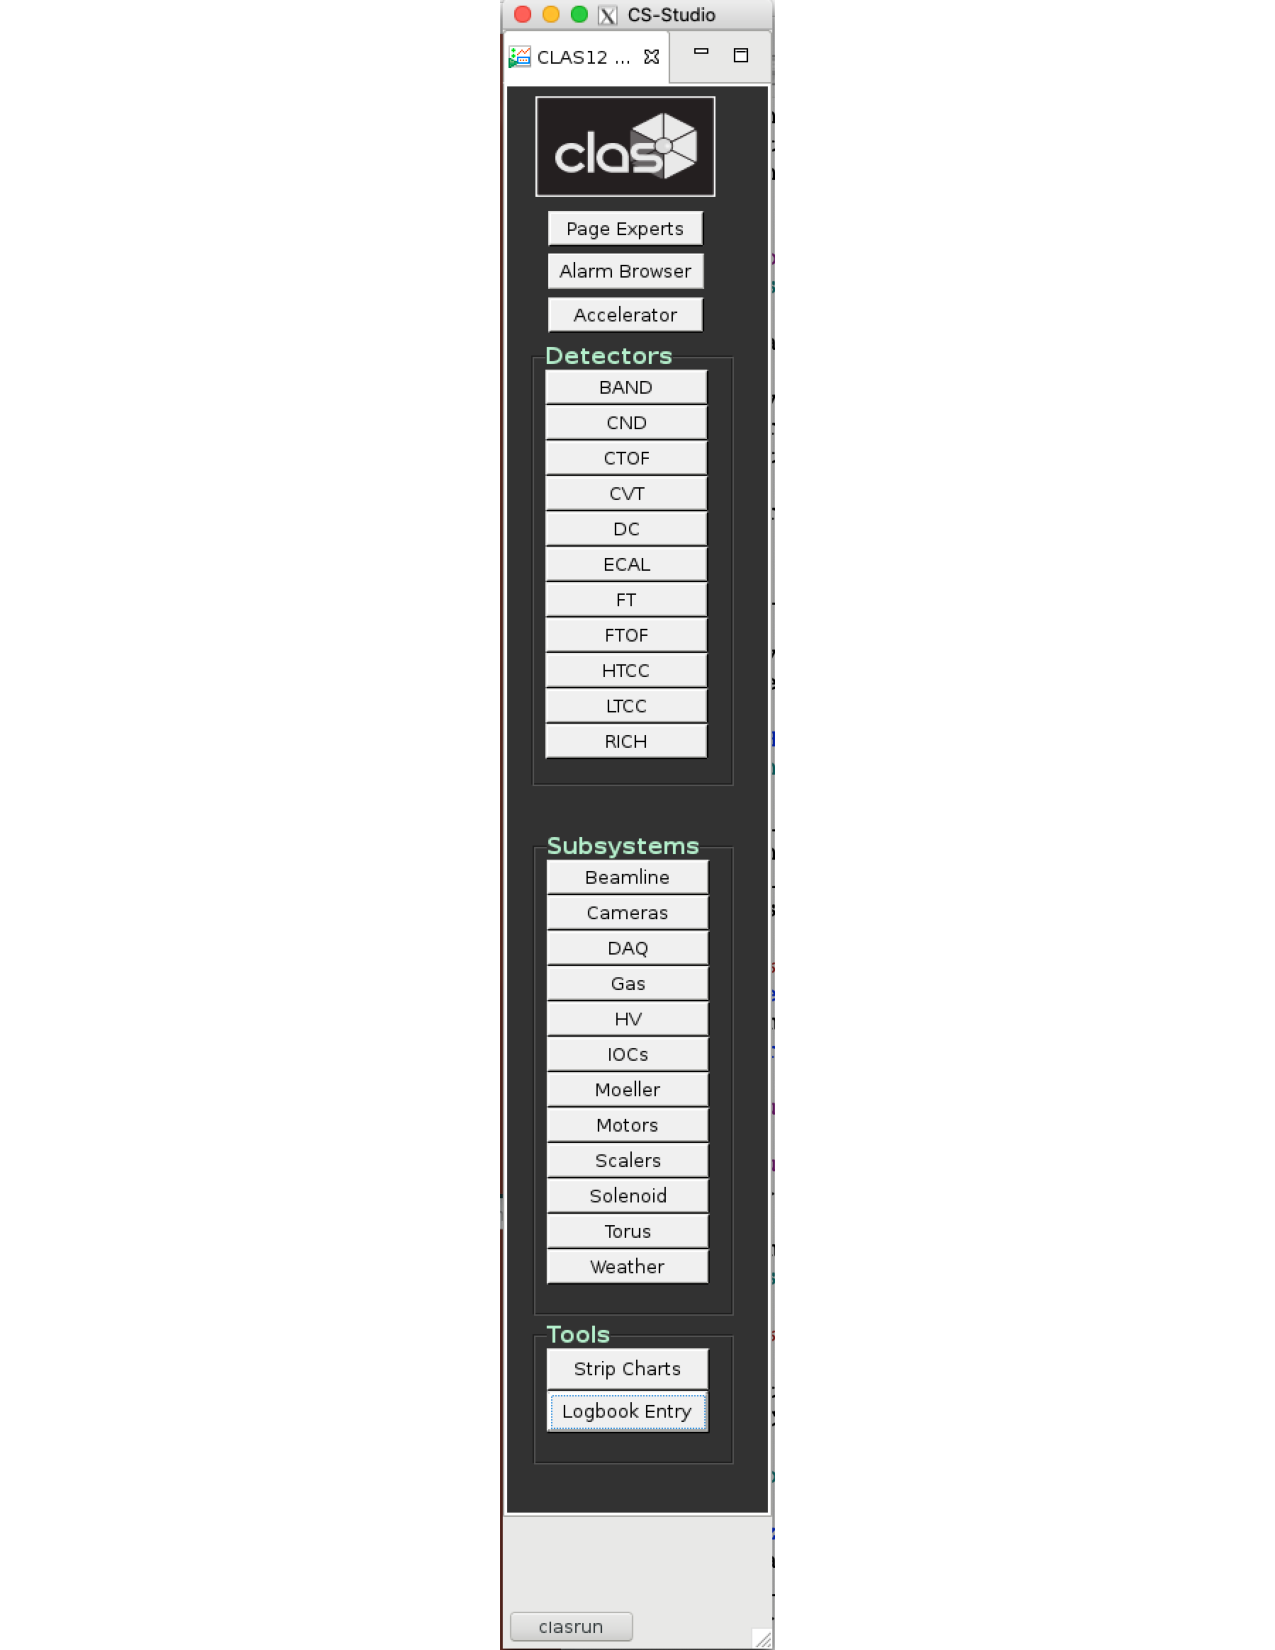
\includegraphics[width=0.50\textwidth,natwidth=610,natheight=642]
{ctof-hv-screen-1.pdf}}}
\put(200,-5)
{\hbox{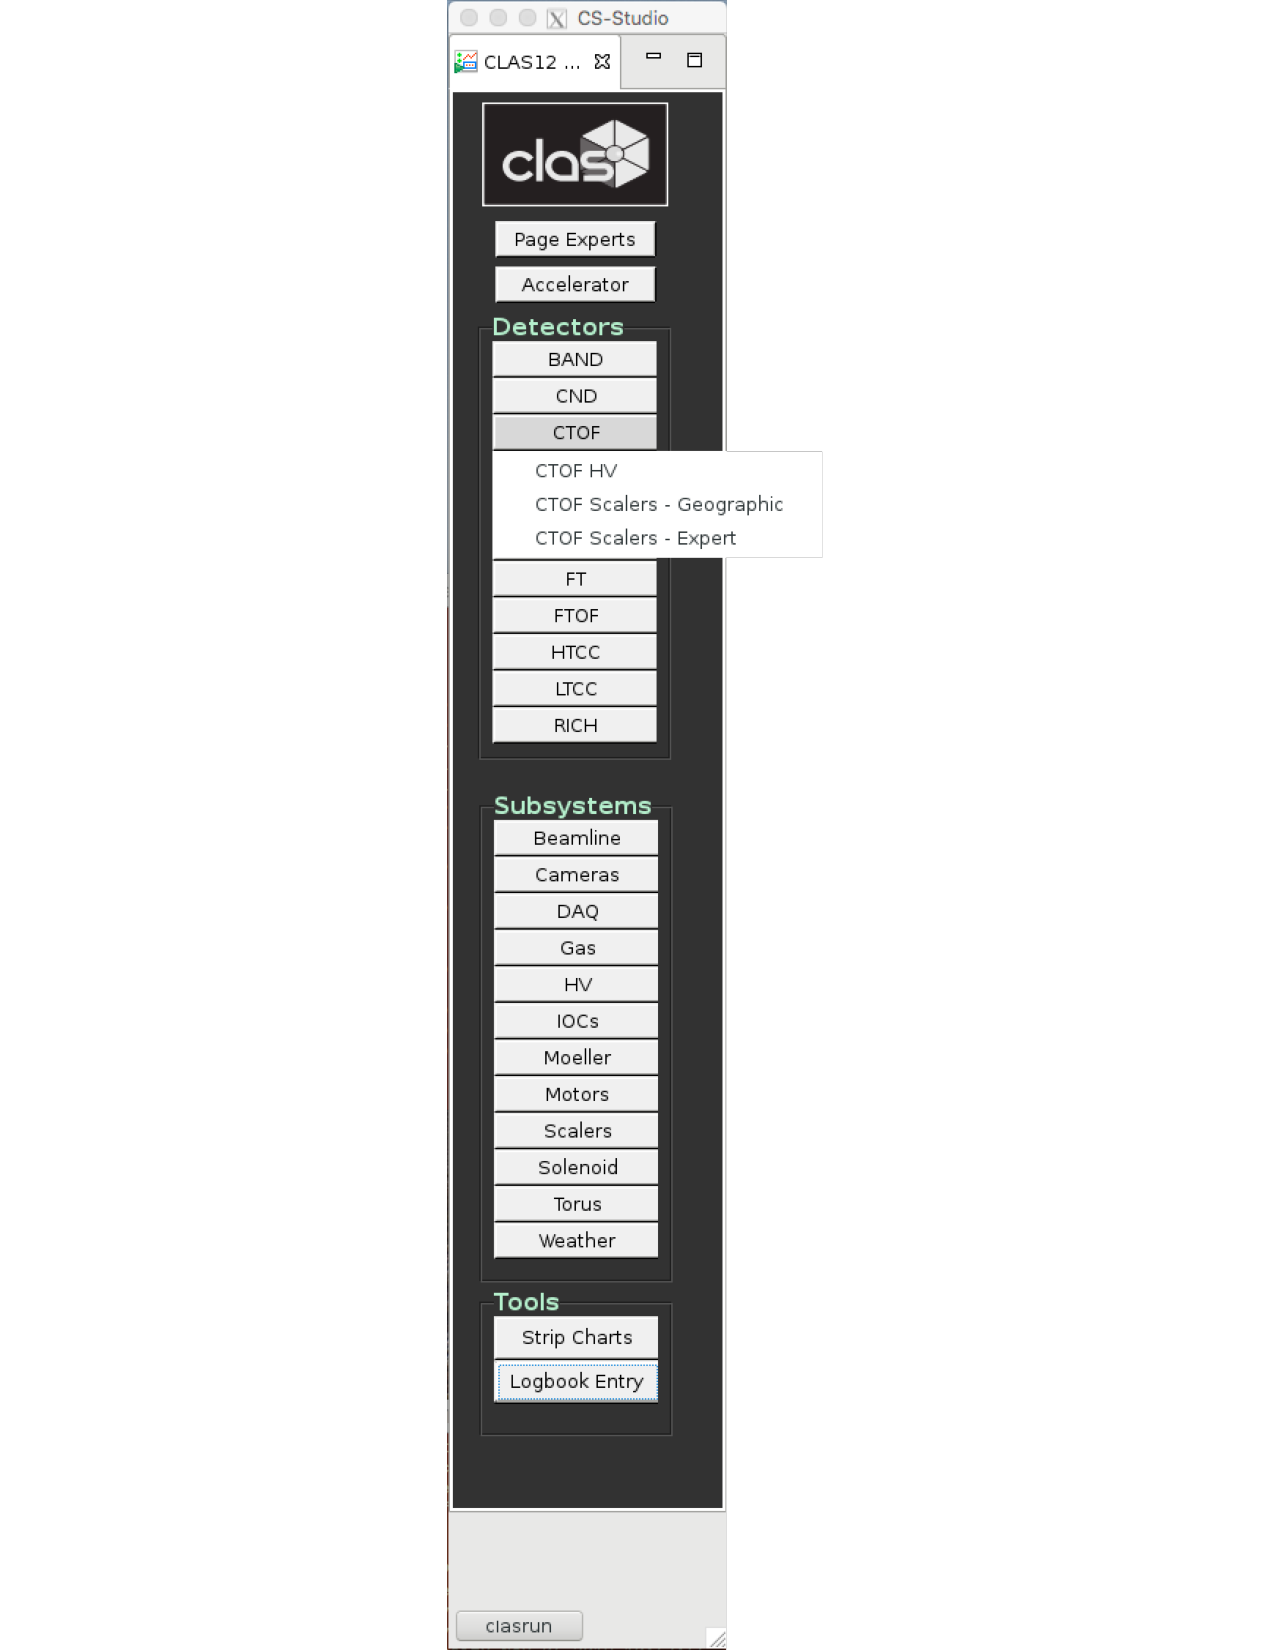
\includegraphics[width=0.50\textwidth,natwidth=610,natheight=642]
{ctof-hv-screen-2.pdf}}}
\end{picture} 
\caption{The CS-Studio interface used for the Slow Controls of the CLAS12 detectors 
and subsystems. (Left) General CLAS12 interface. (Right) Options for the CTOF system.}
\label{ctof-screen1-2}
\end{figure}
%%%%%%%%%%%%%%%%%%%%%%%%%%%%%%%%%%%%%%%%%%%%%%%%%%%%%%%%%%%%%%%%%%%%%%%%%%%%%%%%%%%

To bring up the CTOF HV controls, click on the ``CTOF'' button on the subsystem 
list. This pops up a sub-menu of all Slow Controls subprograms for the CTOF system 
(see Fig.~\ref{ctof-screen1-2}(right)). Clicking the mouse on the ``CTOF HV'' option 
brings up the HV control interface for the CTOF system as shown in 
Fig.~\ref{ctof-screen3-5}(left). This interface allows for HV operations at two 
functionality levels:

\begin{itemize}
\item All channels in the full CTOF system
\item A single PMT in the CTOF system
\end{itemize}

%%%%%%%%%%%%%%%%%%%%%%%%%%%%%%%%%%%%%%%%%%%%%%%%%%%%%%%%%%%%%%%%%%%%%%%%%%%%%%%%%%%
\begin{figure}[htbp]
\vspace{6.5cm}
\begin{picture}(30,50) 
\put(18,-25)
{\hbox{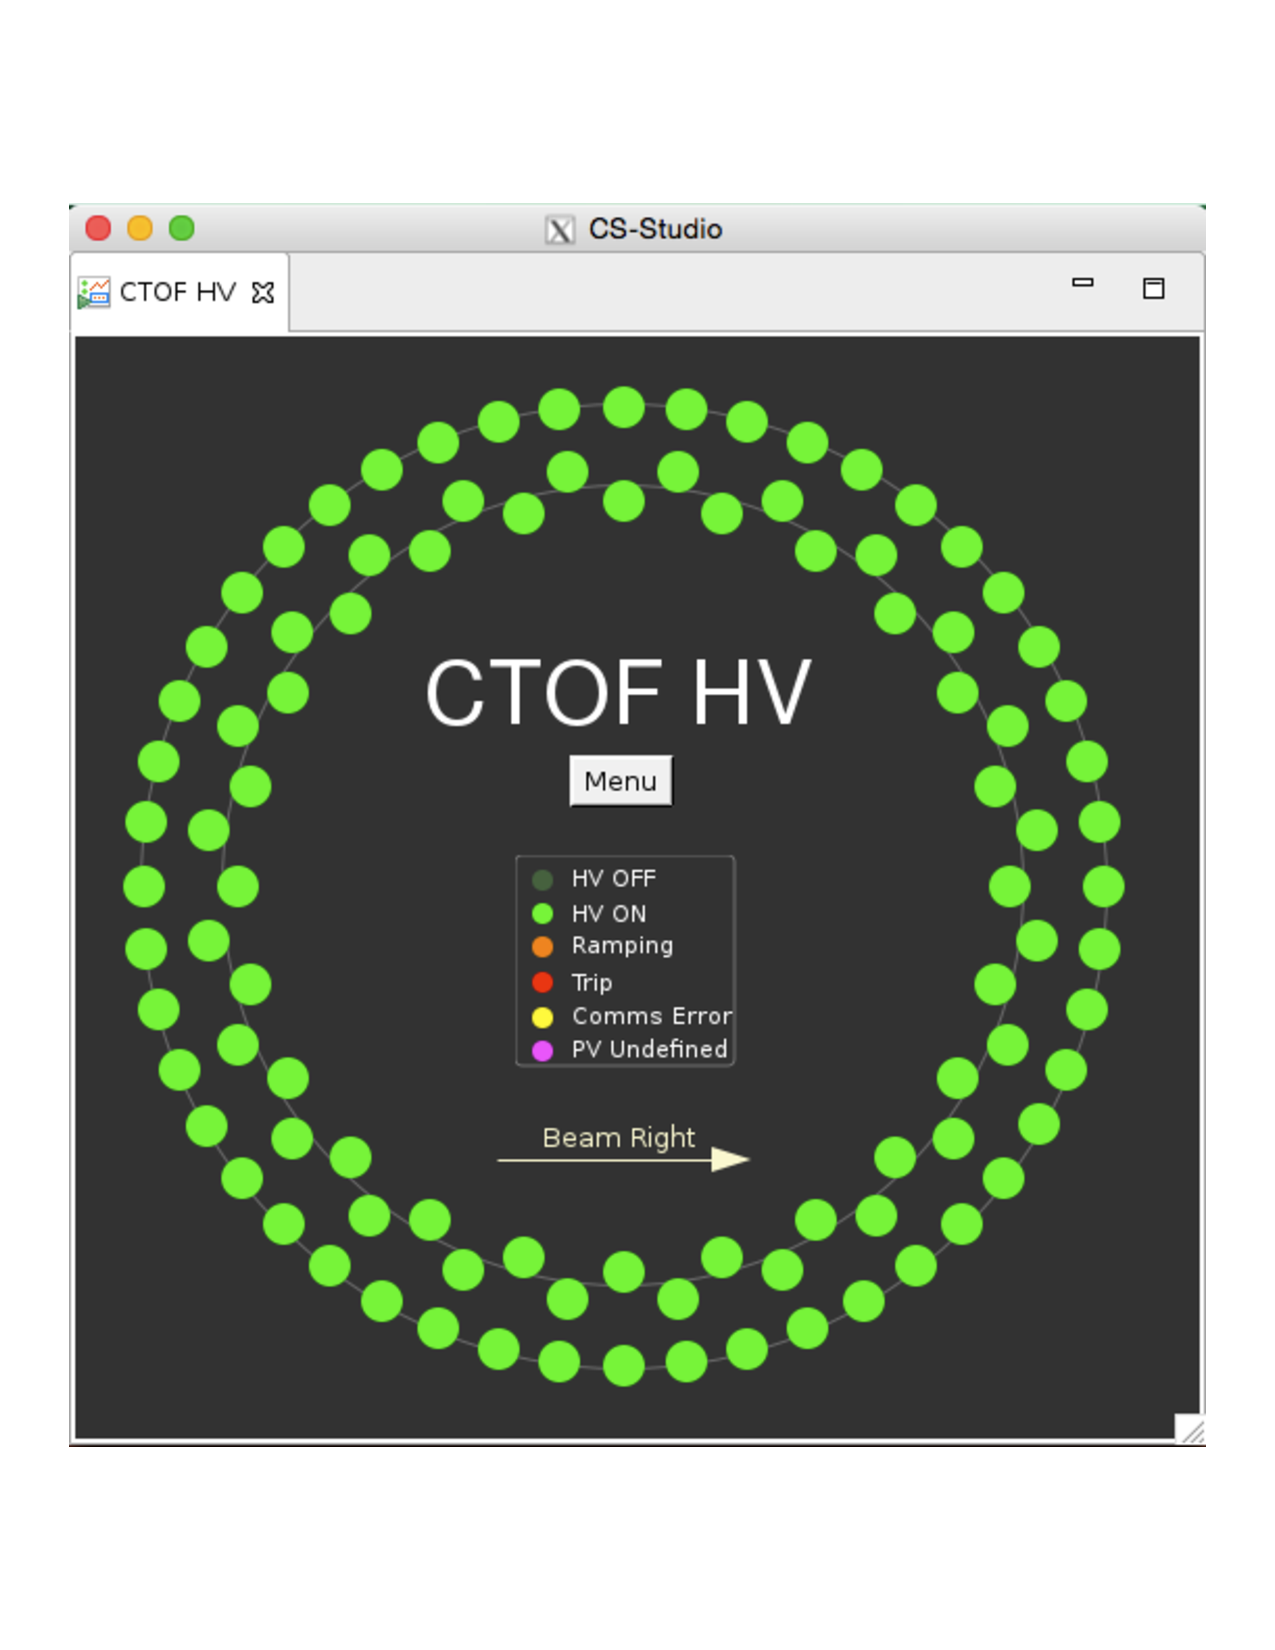
\includegraphics[width=0.45\textwidth,natwidth=610,natheight=642]
{ctof-hv-screen-3.pdf}}}
\put(235,-25)
{\hbox{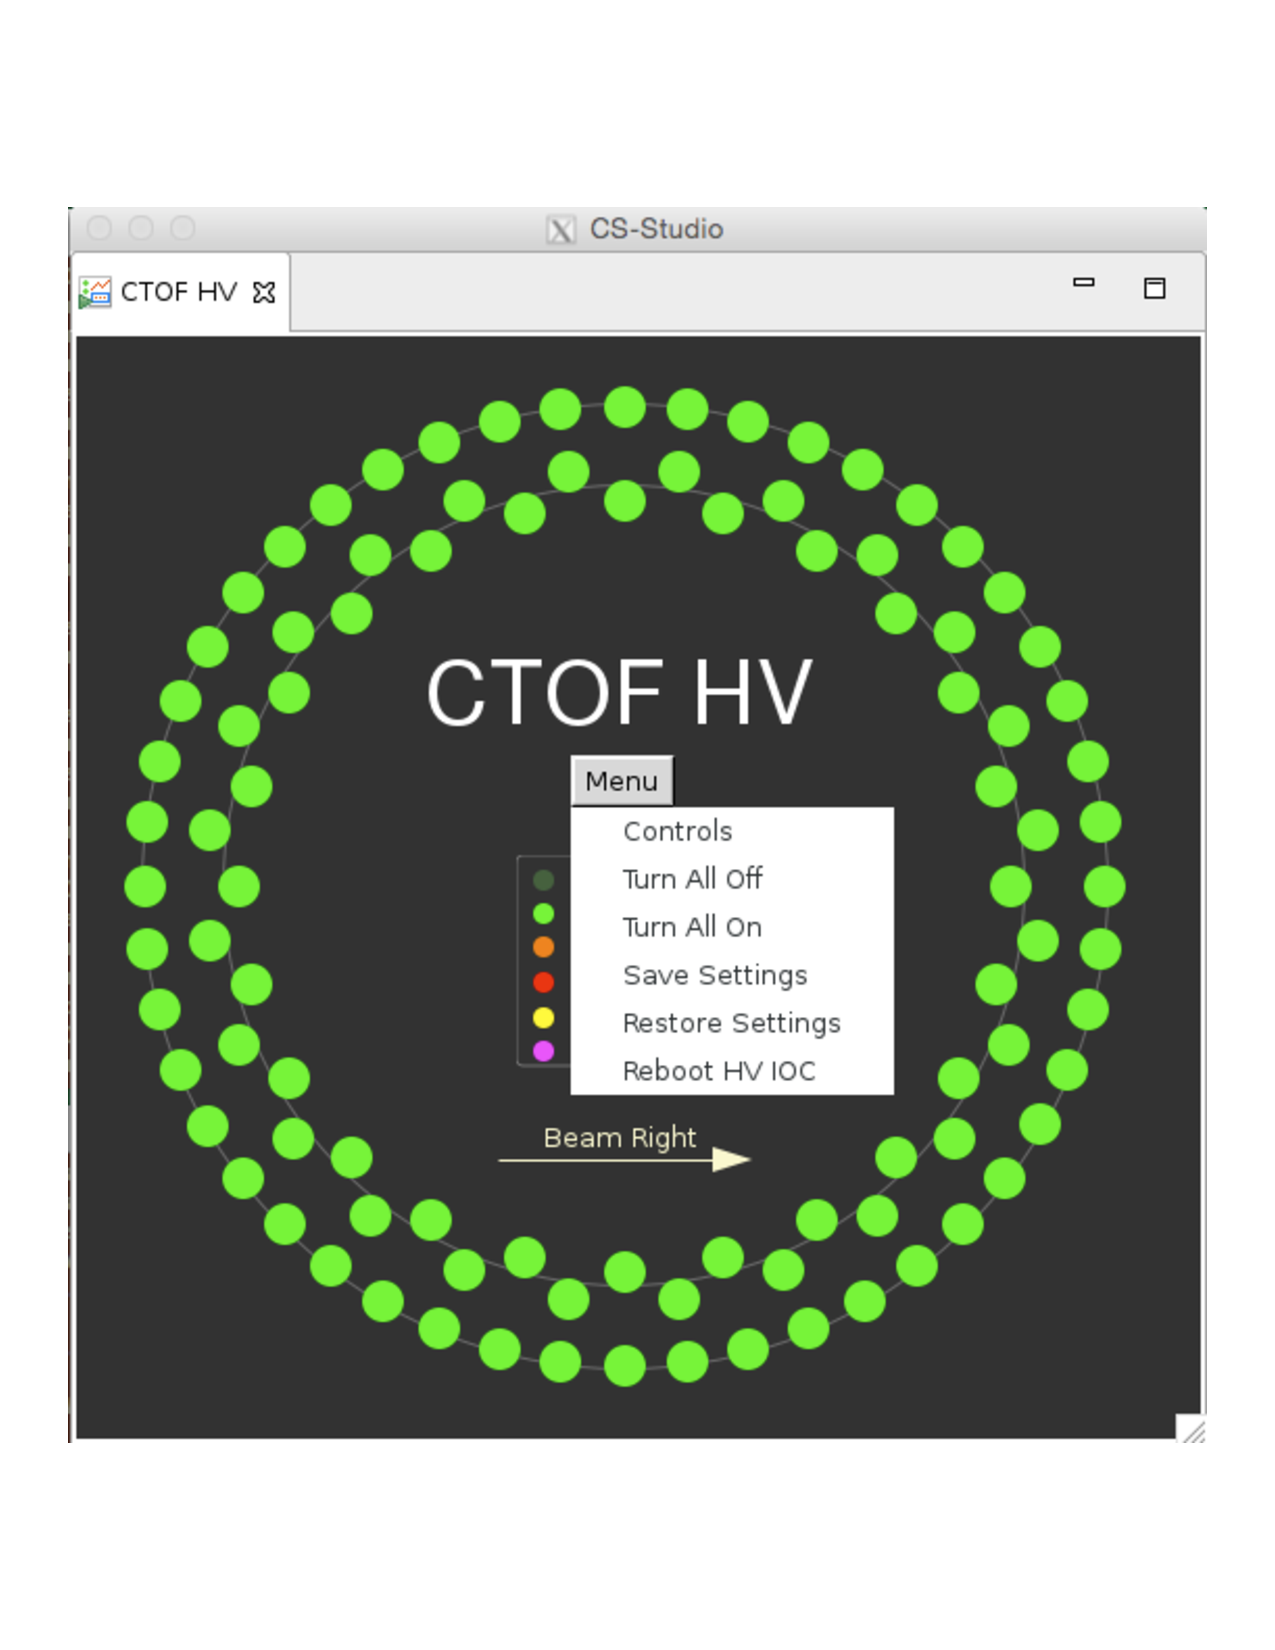
\includegraphics[width=0.45\textwidth,natwidth=610,natheight=642]
{ctof-hv-screen-5.pdf}}}
\end{picture} 
\caption{CTOF HV display and control interface. The right figure shows the ``Menu'' 
options available.}
\label{ctof-screen3-5}
\end{figure}
%%%%%%%%%%%%%%%%%%%%%%%%%%%%%%%%%%%%%%%%%%%%%%%%%%%%%%%%%%%%%%%%%%%%%%%%%%%%%%%%%%%

The HV Control Interface screen (see Fig.~\ref{ctof-screen3-5}) also provides a 
color key to indicate the channel status:

\begin{itemize}
\item HV off - no highlight color (channel color dark green)
\item HV on - bright green
\item HV ramping up or ramping down - orange
\item HV trip - red
\item Communication problem - yellow
\item Undefined channel status - magenta
\end{itemize}

For the shift worker the most common operations are:

\begin{enumerate}
\item To turn the HV for all system PMTs on or off. This is accomplished by clicking 
the ``Menu'' button in the middle of the display. This pops up a sub-menu with the 
relevant options ``Turn All Off'' or ``Turn All On'' (see 
Fig.~\ref{ctof-screen3-5}(right)).
\item To turn individual PMTs on or off. This is accomplished by clicking on the 
circle representing the channel of interest. This brings up a control screen for 
the channel of interest as shown in Fig.~\ref{ctof-screen4}. Clicking on the 
button in the ``Pw'' column toggles the channel HV on and off.
\end{enumerate}

%%%%%%%%%%%%%%%%%%%%%%%%%%%%%%%%%%%%%%%%%%%%%%%%%%%%%%%%%%%%%%%%%%%%%%%%%%%%%%%%%%%
\begin{figure}[htbp]
\vspace{0.2cm}
\begin{picture}(30,50) 
\put(80,150)
{\hbox{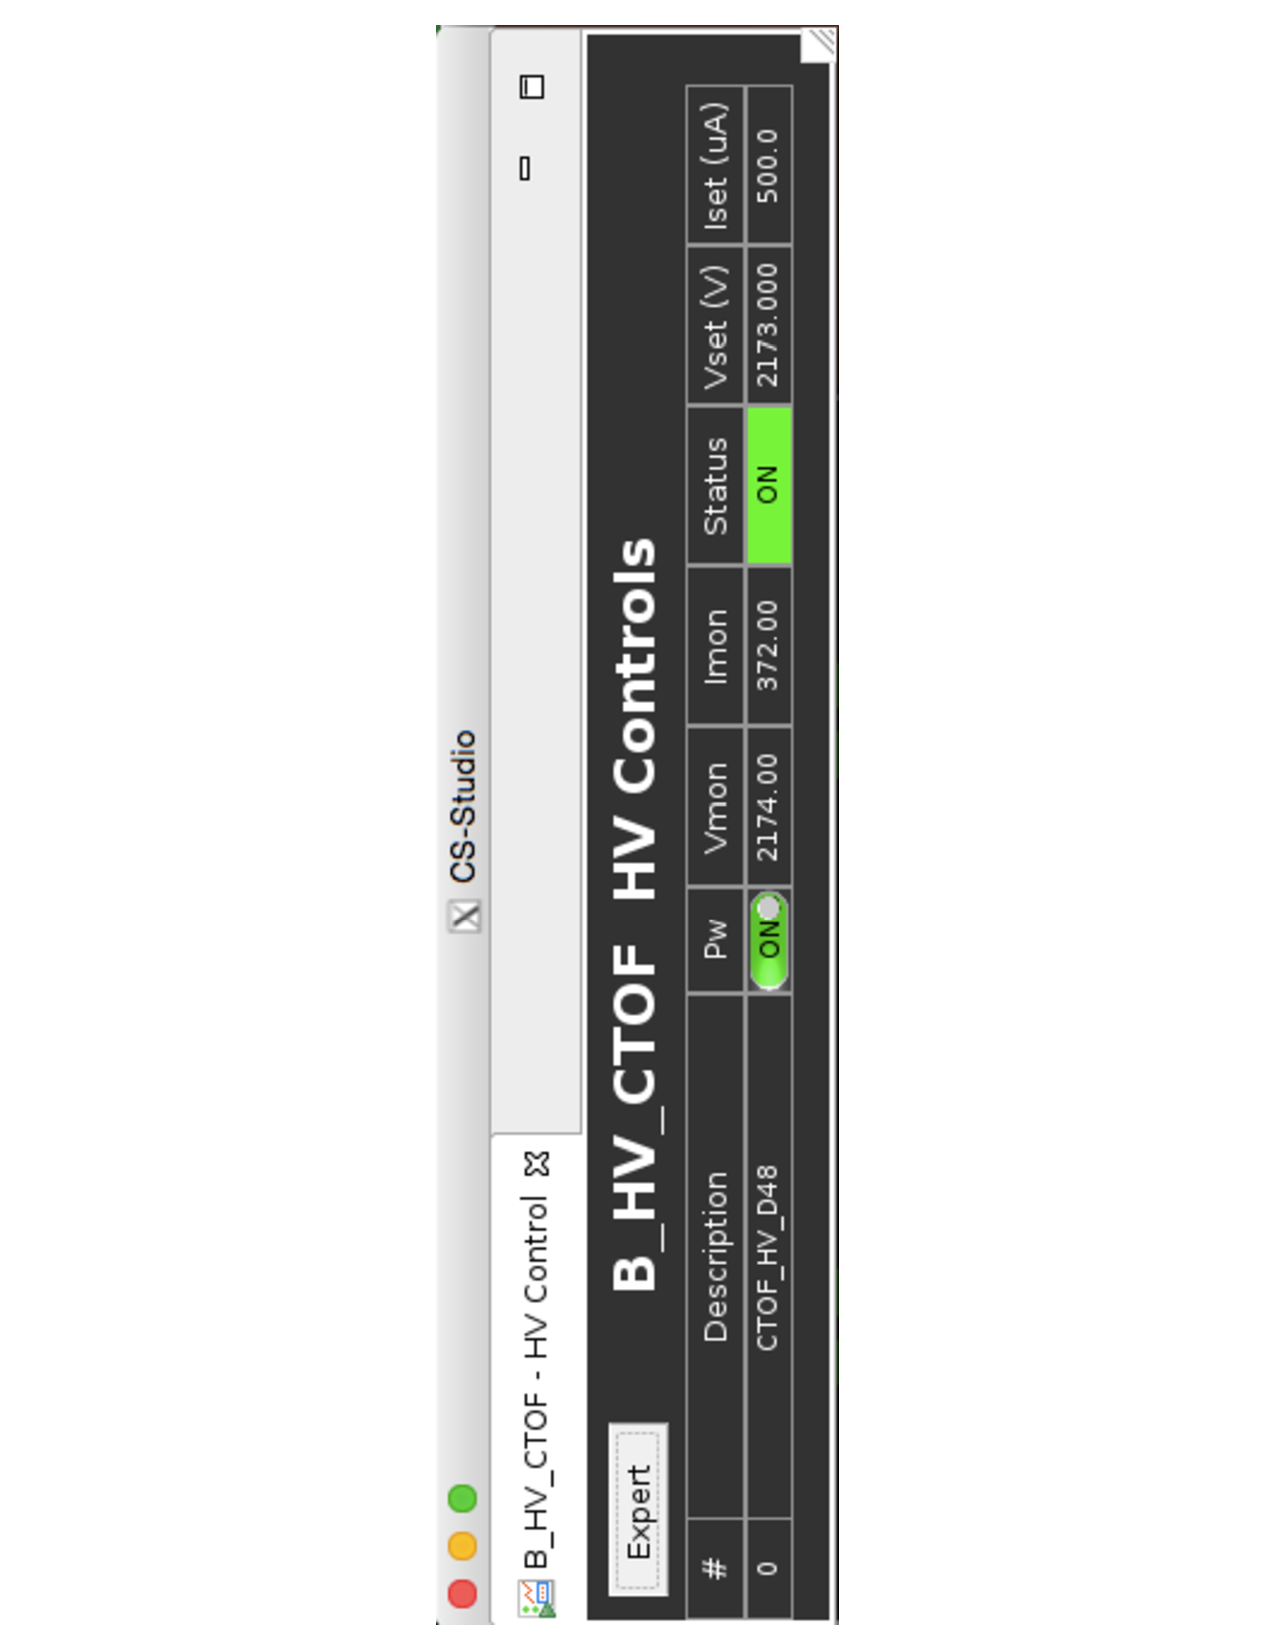
\includegraphics[width=0.50\textwidth,natwidth=610,natheight=642,angle=-90]
{ctof-hv-screen-4.pdf}}}
\end{picture} 
\caption{CTOF HV display for single channel parameters.}
\label{ctof-screen4}
\end{figure}
%%%%%%%%%%%%%%%%%%%%%%%%%%%%%%%%%%%%%%%%%%%%%%%%%%%%%%%%%%%%%%%%%%%%%%%%%%%%%%%%%%%

%%%%%%%%%%%%%%%%%%%%%%%%%%%%%%%%%%%%%%%%%%%%%%%%%%%%%%%%%%%%%%%%%%%%%%%%%%%%%%%%%%%
\begin{figure}[htbp]
\vspace{5.8cm}
\begin{picture}(30,50) 
\put(115,-40)
{\hbox{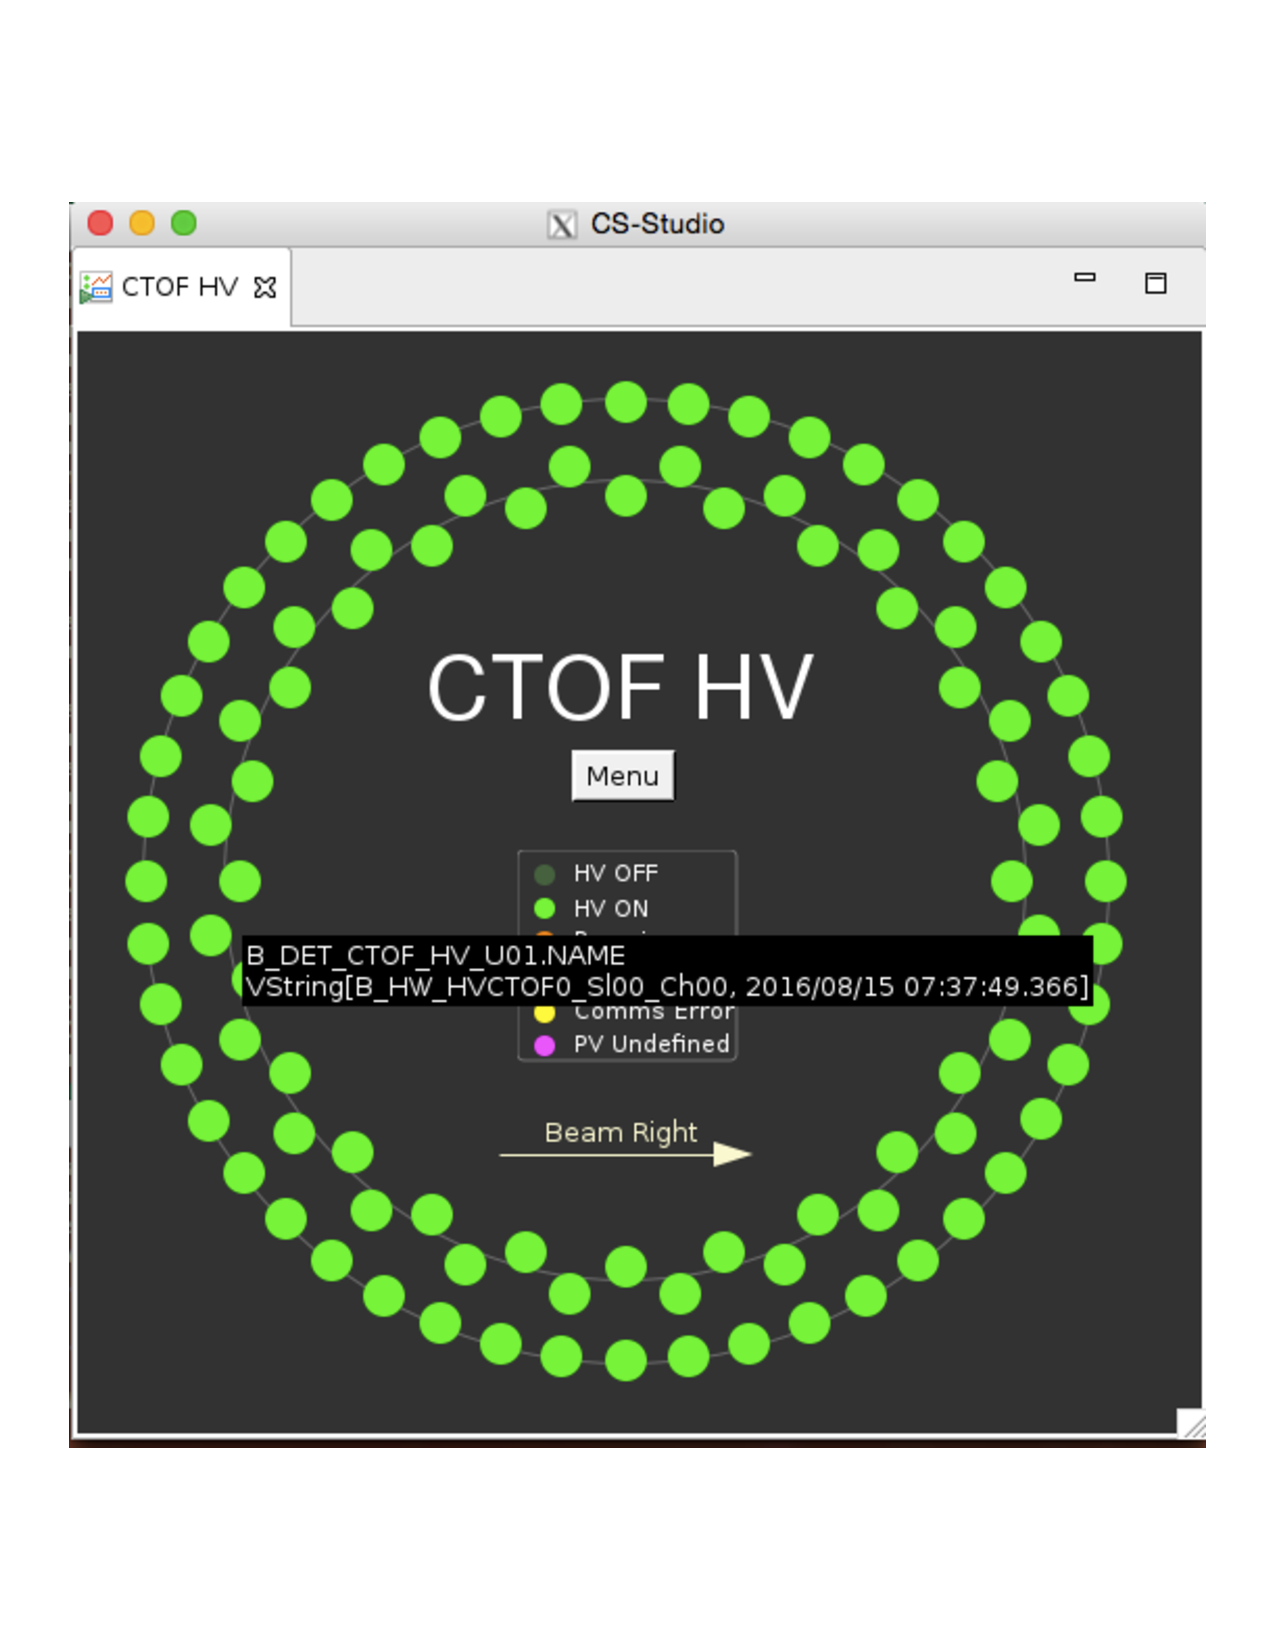
\includegraphics[width=0.50\textwidth,natwidth=610,natheight=642]
{channel-id.pdf}}}
\end{picture} 
\caption{CTOF HV display showing the channel information when the mouse is paused 
over a PMT circle.}
\label{channel-id}
\end{figure}
%%%%%%%%%%%%%%%%%%%%%%%%%%%%%%%%%%%%%%%%%%%%%%%%%%%%%%%%%%%%%%%%%%%%%%%%%%%%%%%%%%%

Note that hovering the mouse pointer on a circle representing a PMT brings up 
information on that channel as shown in Fig.~\ref{channel-id}.

If the ``Controls'' option shown in Fig.~\ref{ctof-screen3-5}(right) is selected, 
a ``novice'' window is opened as shown in Fig.~\ref{ctof-screen6}. This window 
shows the monitored channel voltage and current ($V_{mon}$ (V) and $I_{mon}$ ($\mu$A)), 
the channel status (OFF, ON), and the set channel voltage and current ($V_{set}$ (V) 
and $I_{set}$ ($\mu$A)). If desired, shift workers can toggle the HV settings for 
single channels on or off through this interface.

%%%%%%%%%%%%%%%%%%%%%%%%%%%%%%%%%%%%%%%%%%%%%%%%%%%%%%%%%%%%%%%%%%%%%%%%%%%%%%%%%%%
\begin{figure}[htbp]
\vspace{7.5cm}
\begin{picture}(30,50) 
\put(115,-25)
{\hbox{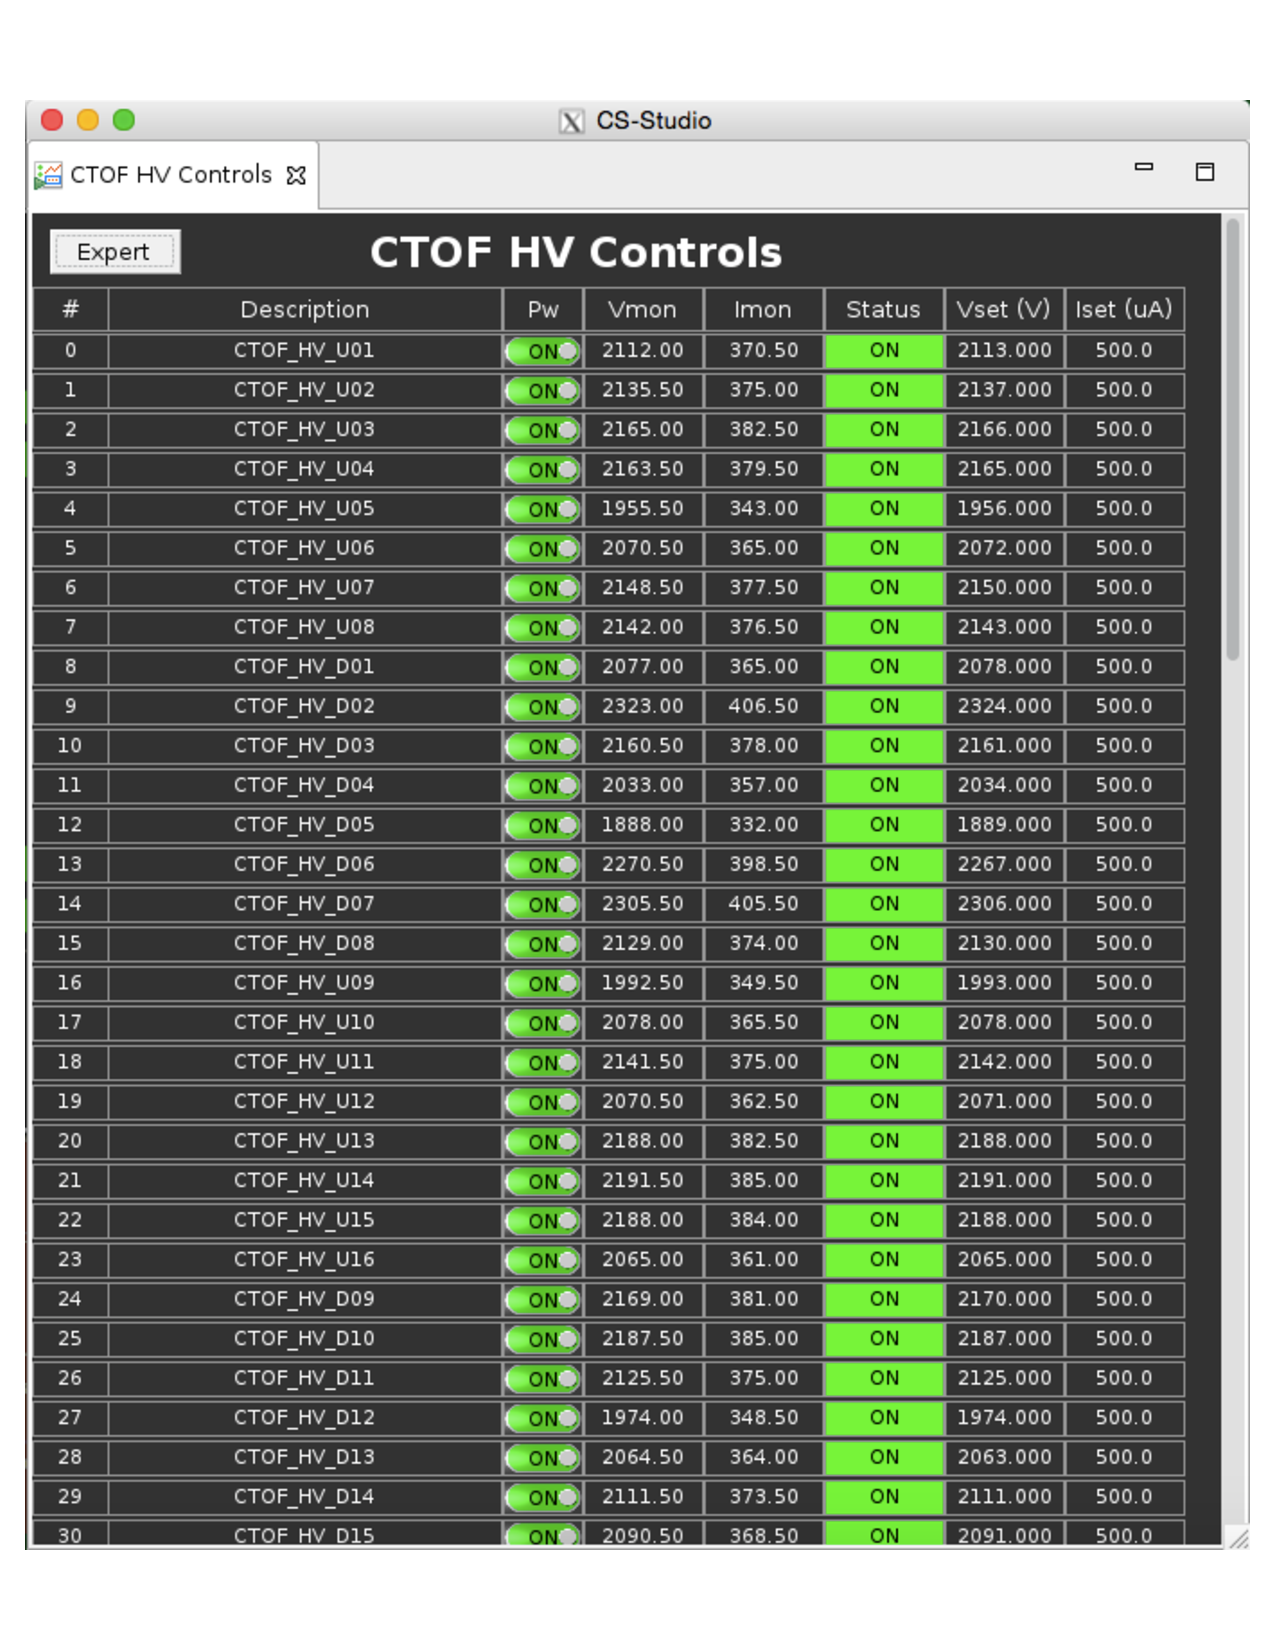
\includegraphics[width=0.50\textwidth,natwidth=610,natheight=642]
{ctof-hv-screen-6.pdf}}}
\end{picture} 
\caption{CTOF ``novice'' channel controls screen.}
\label{ctof-screen6}
\end{figure}
%%%%%%%%%%%%%%%%%%%%%%%%%%%%%%%%%%%%%%%%%%%%%%%%%%%%%%%%%%%%%%%%%%%%%%%%%%%%%%%%%%%

%%%%%%%%%%%%%%%%%%%%%%%%%%%%%%%%%%%%%%%%%%%%%%%%%%%%%%%%%%%%%%%%%%%%%%%%%%%%%%%%%%%
\begin{figure}[htbp]
\vspace{7.0cm}
\begin{picture}(30,50) 
\put(65,265)
{\hbox{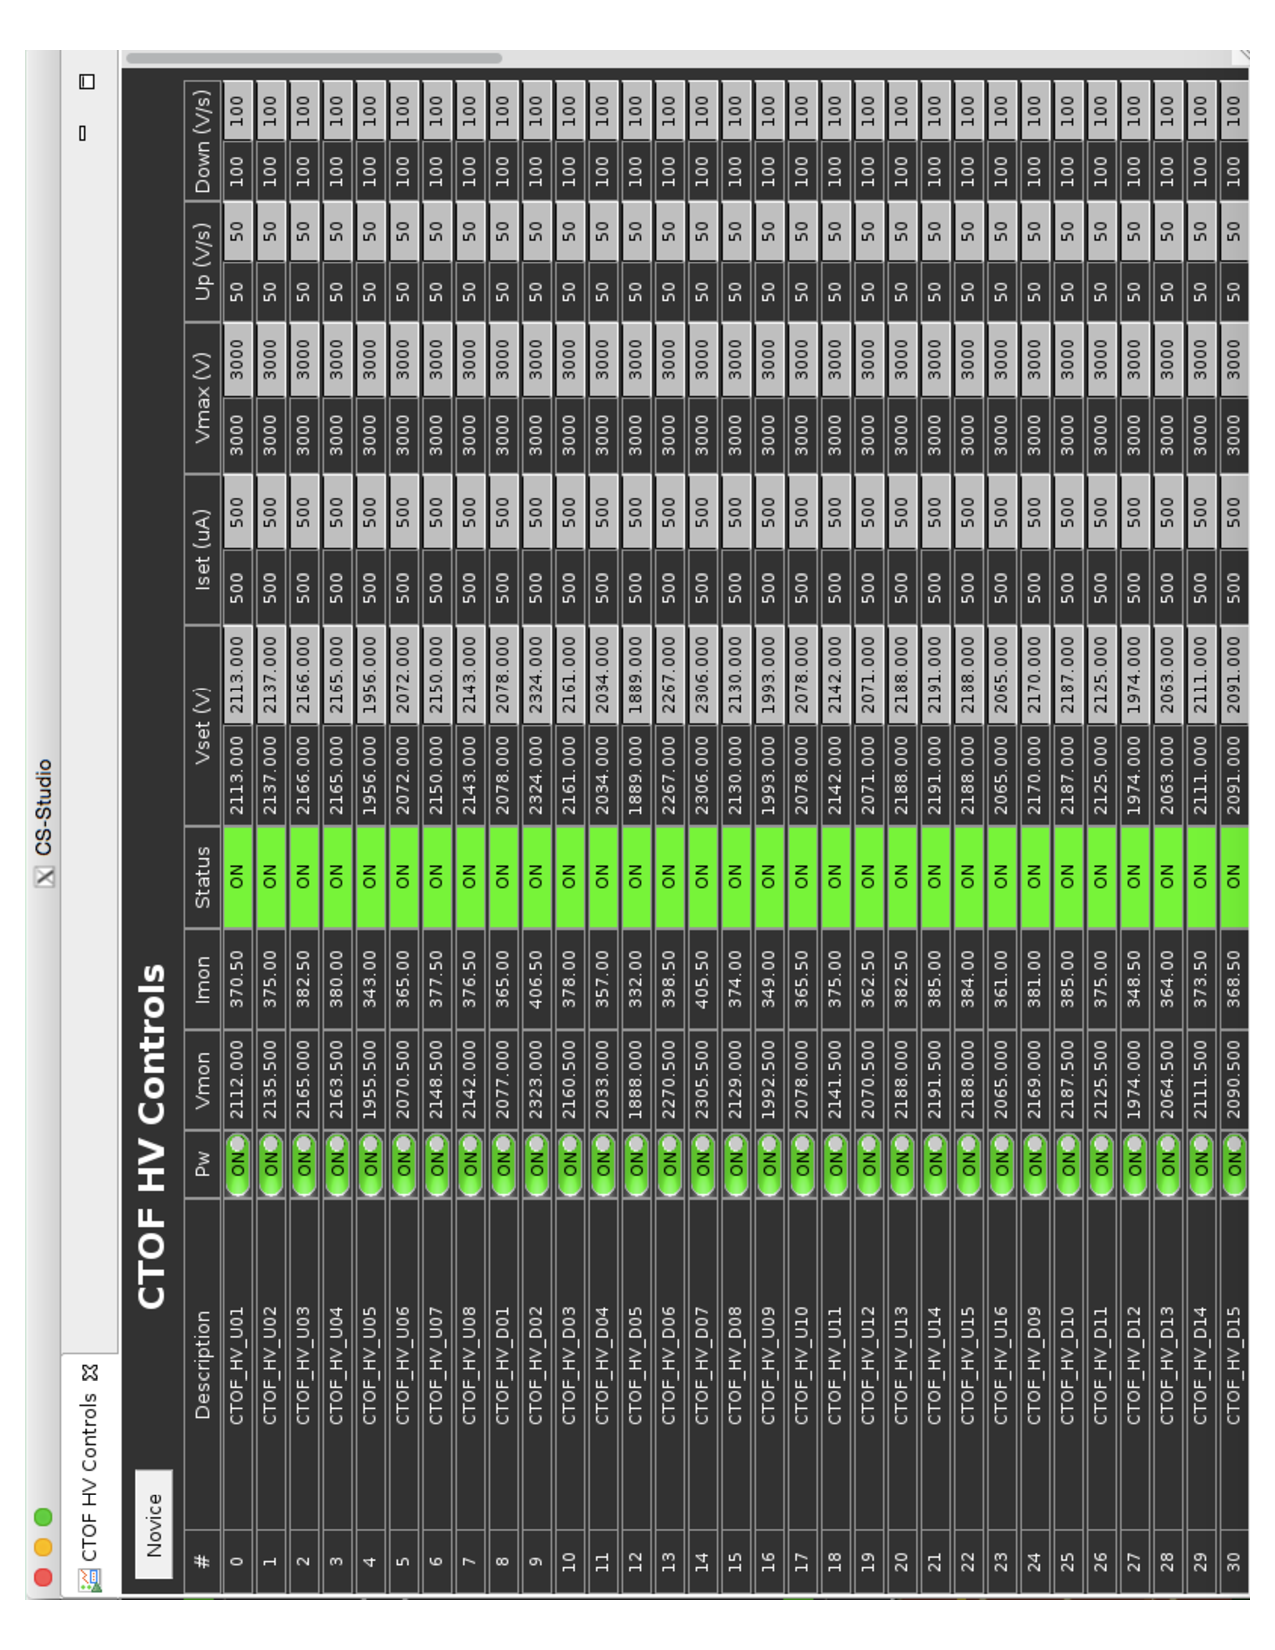
\includegraphics[width=0.57\textwidth,natwidth=610,natheight=642,angle=-90]
{ctof-hv-screen-7.pdf}}}
\end{picture} 
\caption{CTOF ``expert'' channel controls screen.}
\label{ctof-screen7}
\end{figure}
%%%%%%%%%%%%%%%%%%%%%%%%%%%%%%%%%%%%%%%%%%%%%%%%%%%%%%%%%%%%%%%%%%%%%%%%%%%%%%%%%%%

In the upper left corner of this HV Controls window is a button marked ``expert'' 
that brings up the window shown in Fig.~\ref{ctof-screen7}. This window allows 
changes to the system settings for the maximum channel current, maximum channel 
voltage setting, and the channel HV ramp up and ramp down rates. Clicking on the 
``novice'' button in the upper left corner toggles between the expert and novice 
screens. \textcolor{red}{The expert screen should only be used by the authorized 
CTOF personnel listed in Section~\ref{personnel}.} 

\vfil
\eject

\subsubsection{Resetting the IOCs}
\label{reset-iocs}

If there is a controls problem indicated by the appearance of yellow or magenta 
channels in Fig.~\ref{ctof-screen3-5}, which typically appears for all CTOF PMTs, 
the usual cause is an issue of communication between the IOC computer and the HV 
mainframe. To reboot the IOC, click on the ``IOCs'' button on the Slow Controls 
panel within the ``Subsystems'' portion of the interface (see 
Fig.~\ref{ctof-screen1-2}). Fig.~\ref{ioc-reset2} shows the options that appear 
on the sub-menu that pops up. On this menu, select ``HV IOC Health'' to open the 
control window shown in Fig.~\ref{ioc-reset3}. Click on the ``Reboot'' button for 
the HV supply HVCTOF0. The reboot will take less than two minutes to complete and 
the yellow or magenta communication problem channel indicators should all disappear. 
Note that the IOCs can be also rebooted through the CTOF channel control screen 
shown in Fig.~\ref{ctof-screen3-5}(right). Click on the ``Reboot HV IOC'' button 
and answer ``Yes'' on the dialog box that comes up. If rebooting the IOC does not 
solve the communication problems, contact the Slow Controls system expert.

%%%%%%%%%%%%%%%%%%%%%%%%%%%%%%%%%%%%%%%%%%%%%%%%%%%%%%%%%%%%%%%%%%%%%%%%%%%%%%%%%%%
\begin{figure}[ht]
\vspace{8.2cm}
\begin{picture}(30,50) 
\put(130,-5)
{\hbox{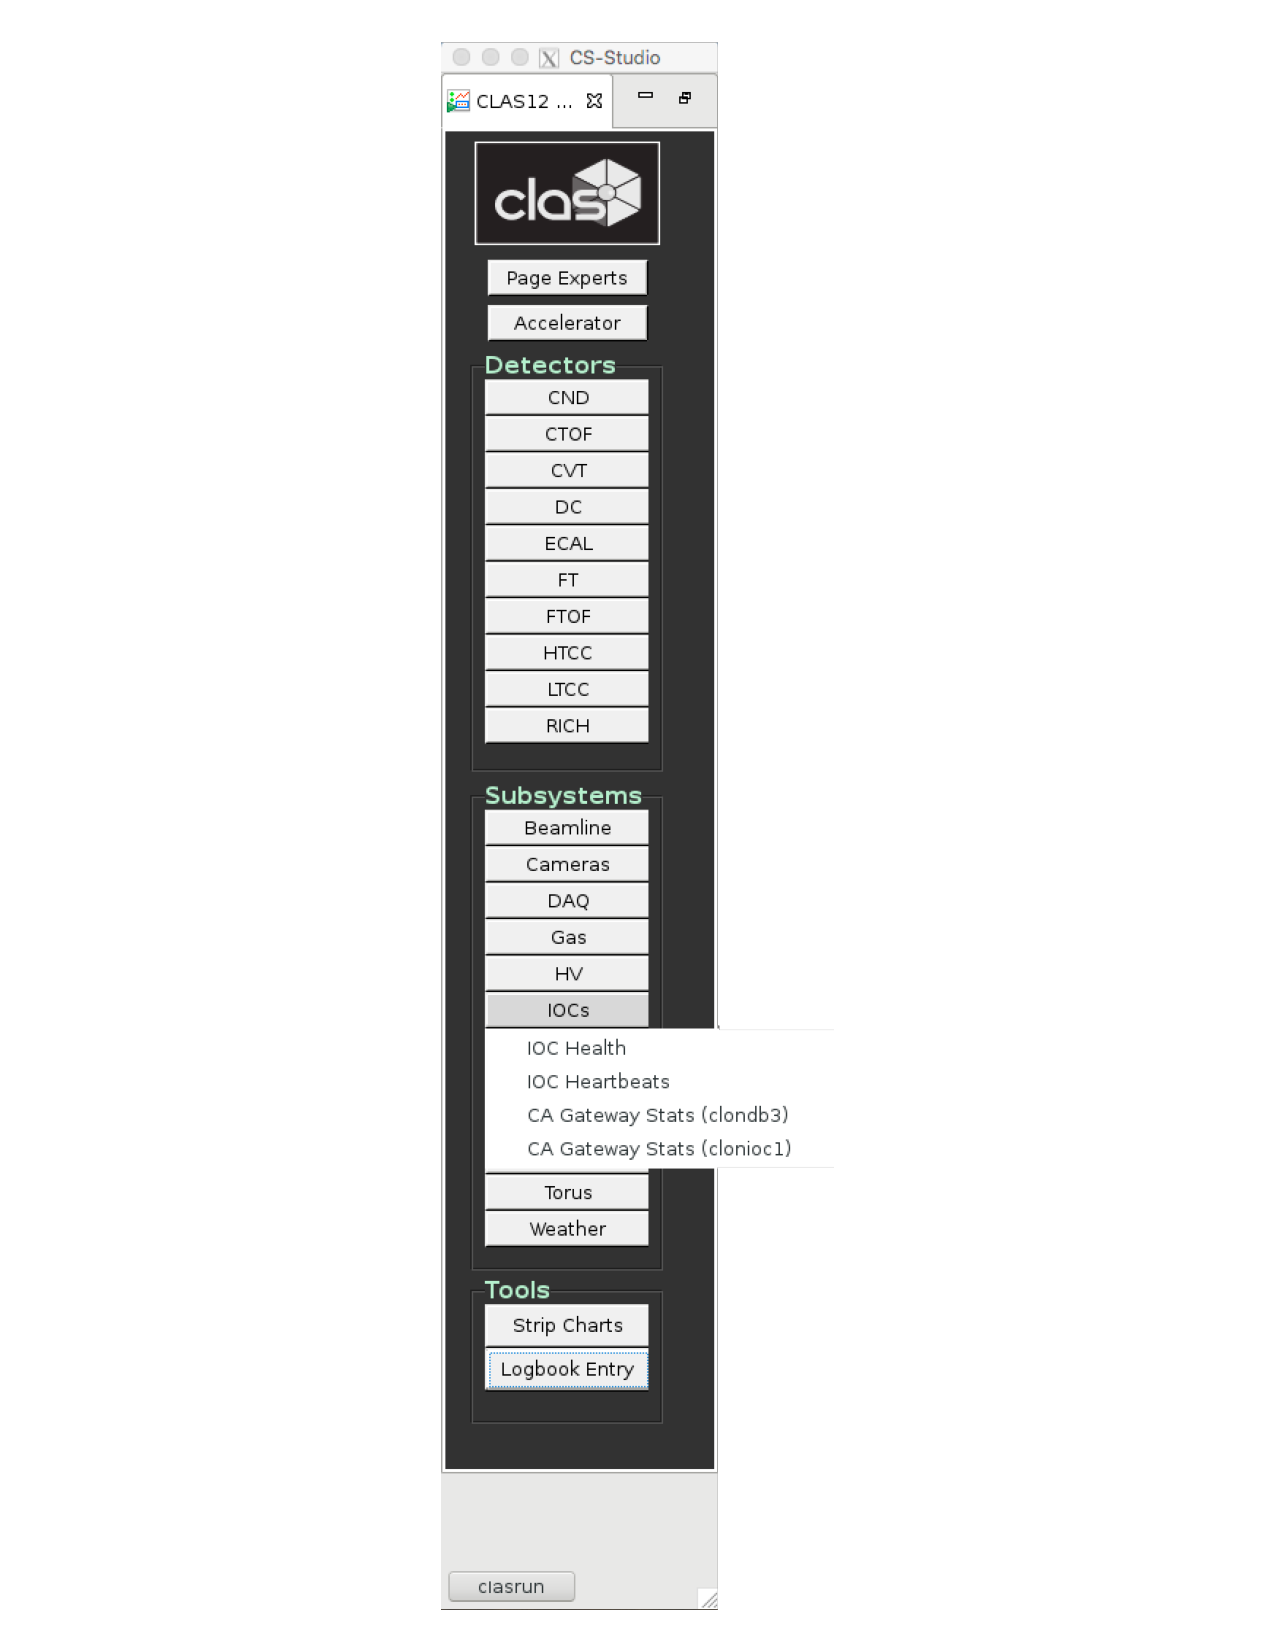
\includegraphics[width=0.50\textwidth,natwidth=610,natheight=642]
{ioc-reset2.pdf}}}
\end{picture} 
\caption{Sub-menu on the primary Slow Controls interface to reboot the IOCs.}
\label{ioc-reset2}
\end{figure}
%%%%%%%%%%%%%%%%%%%%%%%%%%%%%%%%%%%%%%%%%%%%%%%%%%%%%%%%%%%%%%%%%%%%%%%%%%%%%%%%%%%

%%%%%%%%%%%%%%%%%%%%%%%%%%%%%%%%%%%%%%%%%%%%%%%%%%%%%%%%%%%%%%%%%%%%%%%%%%%%%%%%%%%
\begin{figure}[htbp]
\vspace{3.0cm}
\begin{picture}(30,50) 
\put(60,210)
{\hbox{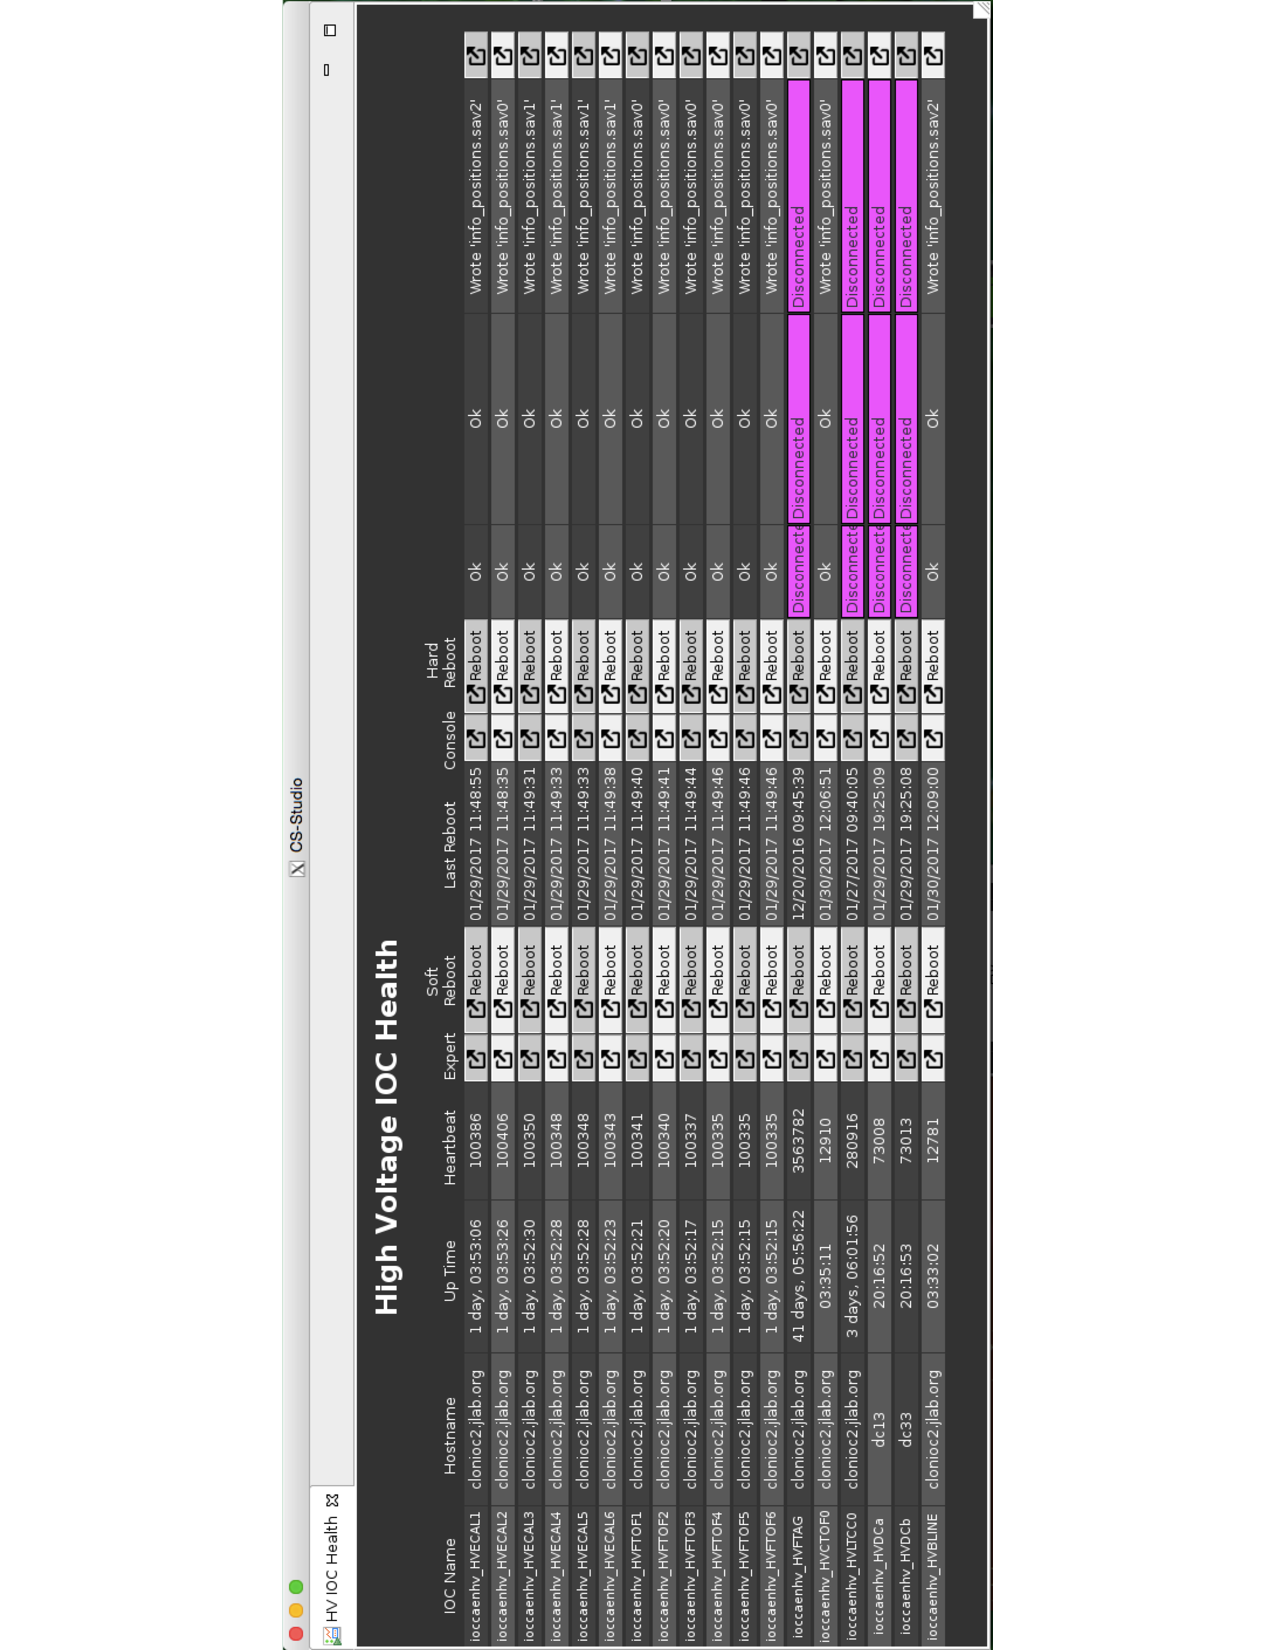
\includegraphics[width=0.57\textwidth,natwidth=610,natheight=642,angle=-90]
{ioc-reset3.pdf}}}
\end{picture} 
\caption{HV IOC health screen where individual IOCs can be rebooted.}
\label{ioc-reset3}
\end{figure}
%%%%%%%%%%%%%%%%%%%%%%%%%%%%%%%%%%%%%%%%%%%%%%%%%%%%%%%%%%%%%%%%%%%%%%%%%%%%%%%%%%%

\clearpage

\vfil
\eject

\subsection{Low Voltage Controls for Shield Compensation Coils}
\label{comp-coils}

The PMT active magnetic shield layer consists of two independent coils, the 
first $z_1$ of 90 turns placed about the middle of the PMT accelerating structure 
and the second $z_2$ of 60 turns placed about the PMT photocathode (see 
Fig.~\ref{coil-layout}). Coil currents on the order of 0.5 - 1~A are sufficient 
to reduce the inner remnant magnetic field within the PMT shield system of 0.5 - 
1~G down to the level of 0.2 - 0.3~G.

%%%%%%%%%%%%%%%%%%%%%%%%%%%%%%%%%%%%%%%%%%%%%%%%%%%%%%%%%%%%%%%%%%%%%%%%%%%%%%%%%%%
\begin{figure}[htbp]
\vspace{1.5cm}
\begin{picture}(50,50) 
\put(80,-155)
{\hbox{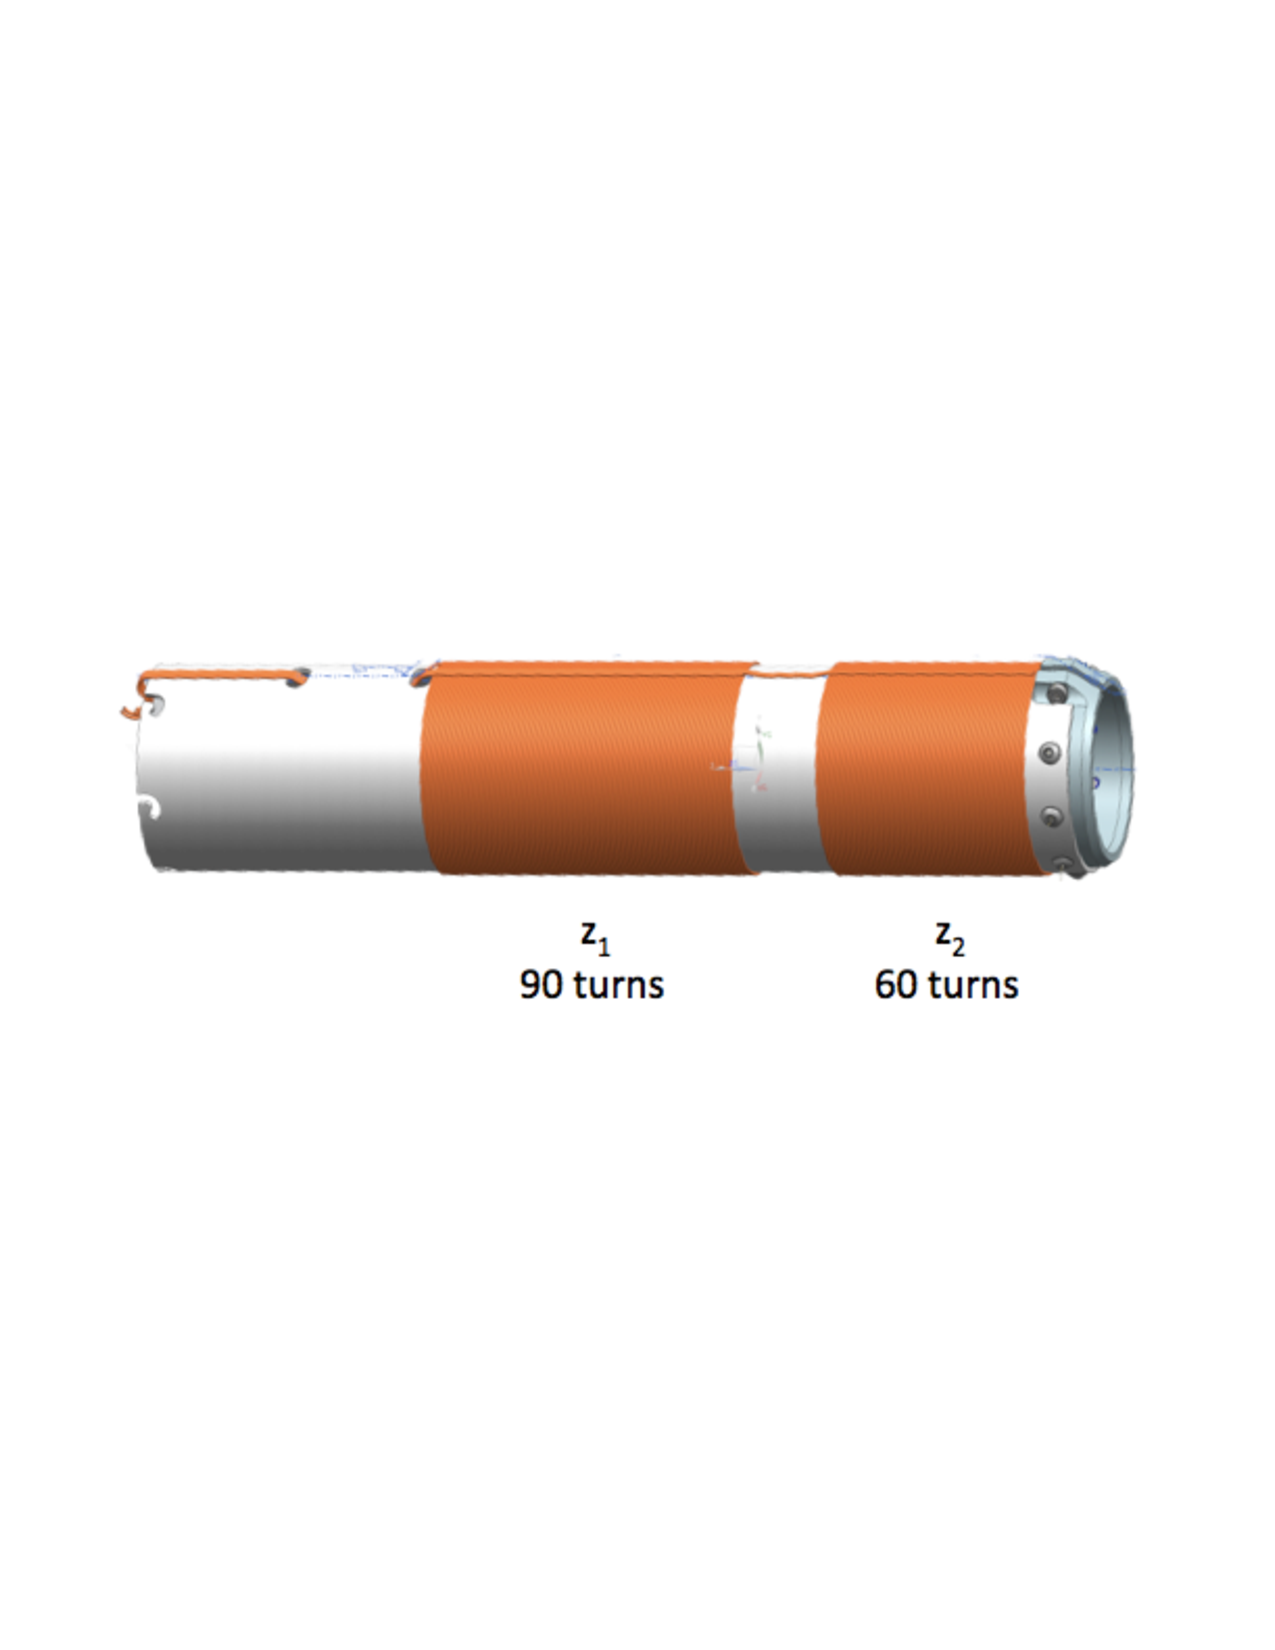
\includegraphics[width=0.65\textwidth,natwidth=610,natheight=642]
{coil-layout.pdf}}}
\end{picture} 
\caption{Model layout of the compensation coils on the shield mandrel showing the 
coil $z_1$ with 90 turns and coils $z_2$ with 60 turns. $z_1$ spans the middle to 
back part of the PMT dynode structure and $z_2$ spans the region about the PMT 
photocathode.}
\label{coil-layout}
\end{figure}
%%%%%%%%%%%%%%%%%%%%%%%%%%%%%%%%%%%%%%%%%%%%%%%%%%%%%%%%%%%%%%%%%%%%%%%%%%%%%%%%%%%

For the CTOF shields the compensation coils $z_1$ and $z_2$ are independently 
controllable. The LV power supply for the coils is a Wiener MPOD mini-crate 
outfitted with two MPV8016I modules. Each module has eight channels that can 
individually provide up to 50~W per channel with a maximum current of 5~A. The 
power supply is connected to the coils via 52 - 68~ft long cables. Each supply 
channel feeds 12 coils. The system has been tuned for six different values of 
currents in $z_1$ and $z_2$ corresponding to the upstream low-pitch angle shields, 
the upstream high-pitch angle shields, and the downstream shields. Fig.~\ref{coils} 
shows the power circuit layout.

%%%%%%%%%%%%%%%%%%%%%%%%%%%%%%%%%%%%%%%%%%%%%%%%%%%%%%%%%%%%%%%%%%%%%%%%%%%%%%%%%%%
\begin{figure}[htbp]
\vspace{9.5cm}
\begin{picture}(50,50) 
\put(30,325)
{\hbox{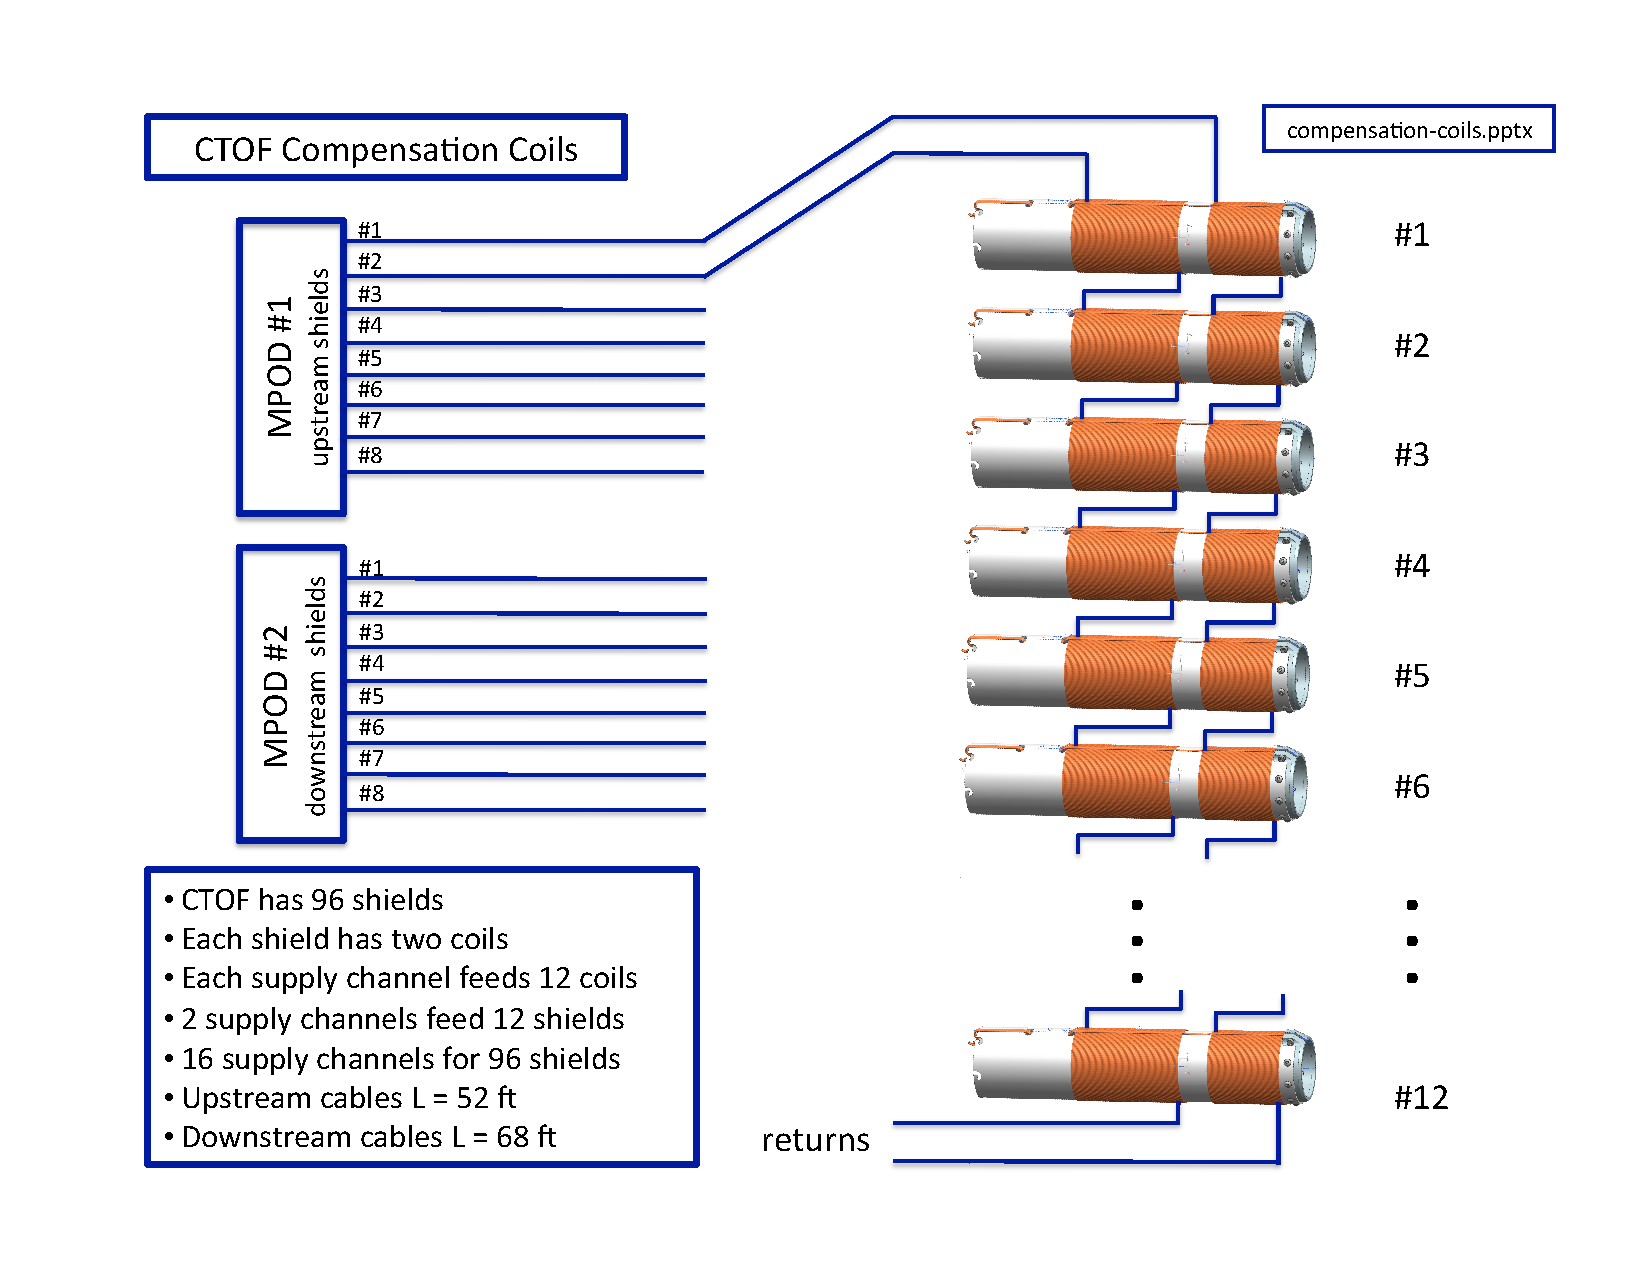
\includegraphics[width=0.70\textwidth,natwidth=610,natheight=642,angle=-90]
{compensation-coils.pdf}}}
\end{picture} 
\caption{Layout of the power circuit for the CTOF magnetic shield compensation 
coils.}
\label{coils}
\end{figure}
%%%%%%%%%%%%%%%%%%%%%%%%%%%%%%%%%%%%%%%%%%%%%%%%%%%%%%%%%%%%%%%%%%%%%%%%%%%%%%%%%%%

Although the Wiener MPOD system can provide up to 5~A per channel, the typical 
coil currents are at the level of 0.5 - 1~A. In this current regime the coil 
system remains at room temperature. During operation of the coil power supply in 
Hall~B, a temperature interlock circuit protects the coils from overheating. An 
over-temperature condition shuts down the Wiener LV supply whose status is monitored 
by the Hall~B alarm handler.

The Wiener MPOD power supply control interface is brought up through the CTOF control 
panel shown in Fig.~\ref{ctof-screen1-2} by clicking on the option ``CTOF LV''. The 
screen that comes up is shown in Fig.~\ref{ctof-lv-control}. Note that a communication 
problem between the controls and the power supply would be indicated by magenta colors 
on the associated channels. To reboot the IOC, follow the instructions in 
Section~\ref{reset-iocs}. If problems with communications remain after rebooting
the IOC, contact the Slow Controls expert.

%%%%%%%%%%%%%%%%%%%%%%%%%%%%%%%%%%%%%%%%%%%%%%%%%%%%%%%%%%%%%%%%%%%%%%%%%%%%%%%%%%%
\begin{figure}[htbp]
\vspace{2.5cm}
\begin{picture}(30,50) 
\put(25,250)
{\hbox{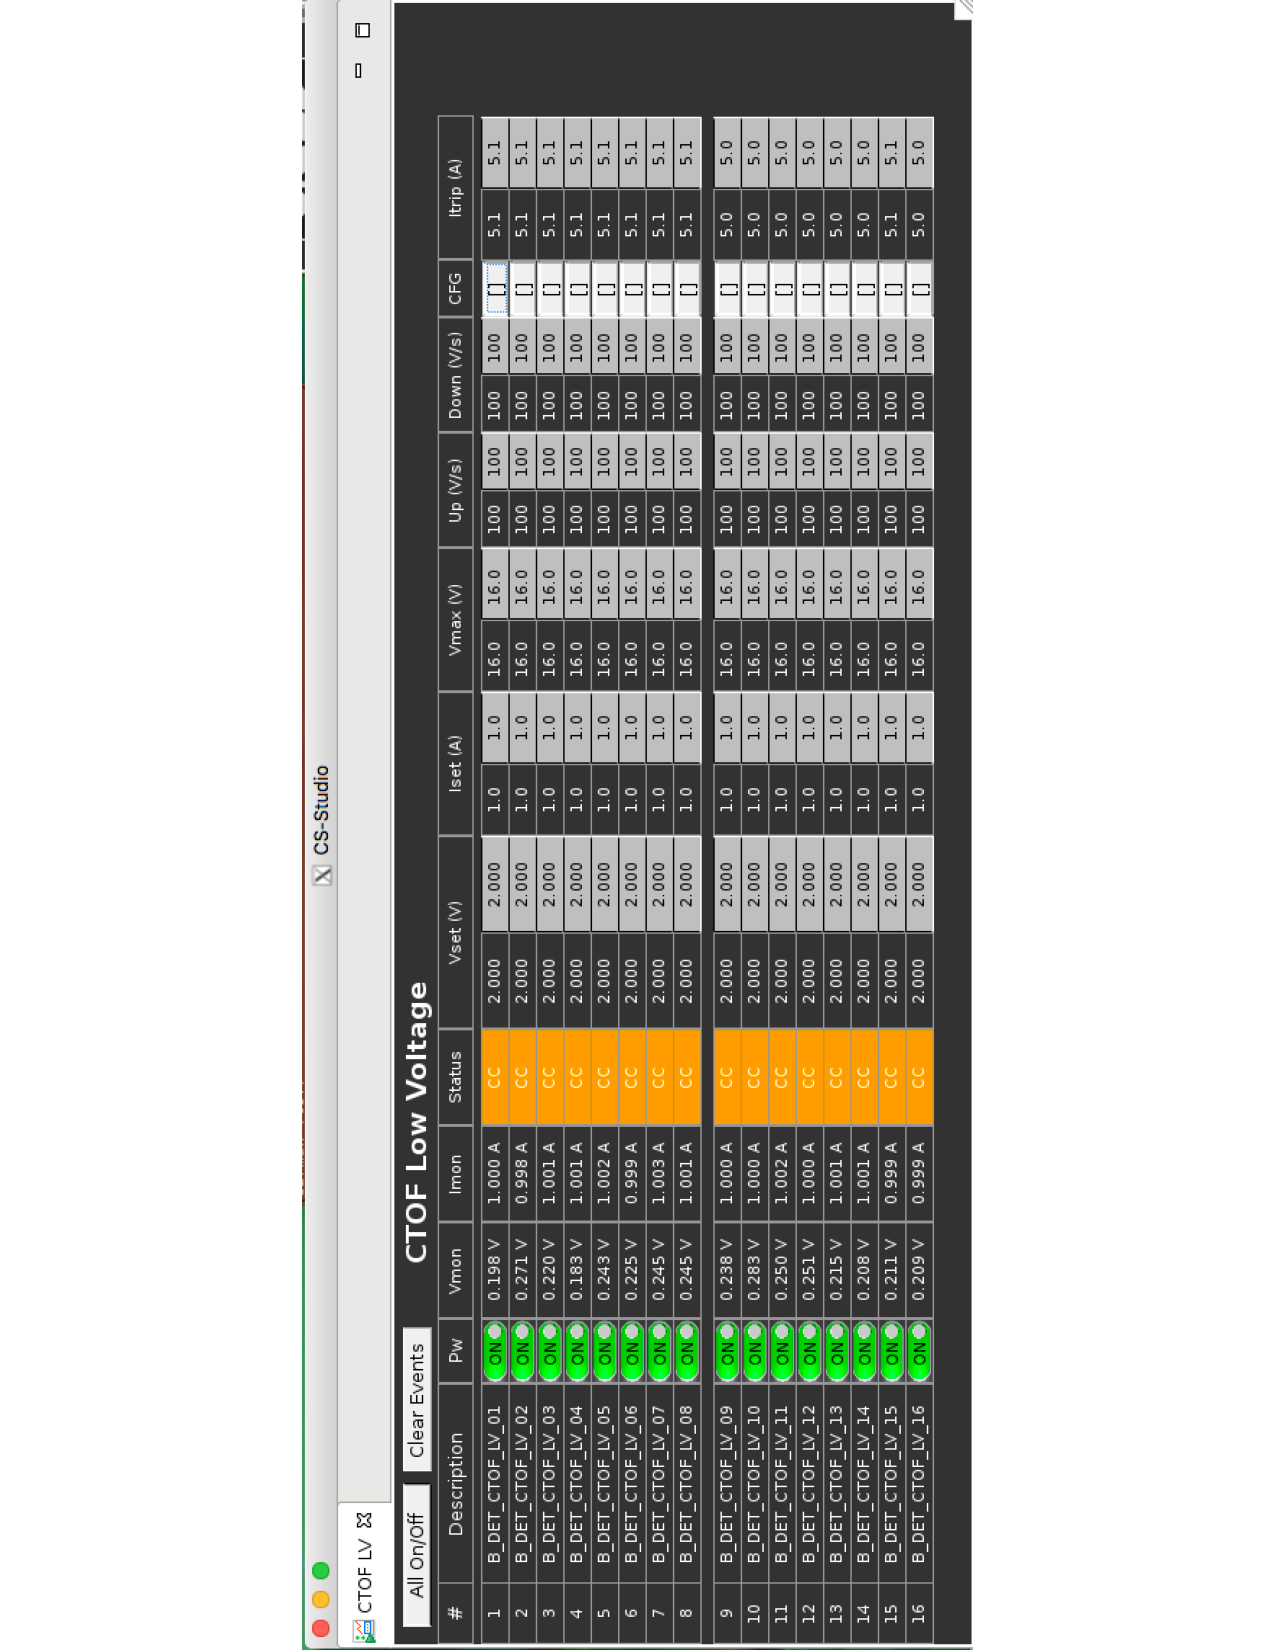
\includegraphics[width=0.70\textwidth,natwidth=610,natheight=642,angle=-90]
{ctof-lv-control.pdf}}}
\end{picture} 
\caption{Low voltage system control interface model for the CTOF compensation coils.}
\label{ctof-lv-control}
\end{figure}
%%%%%%%%%%%%%%%%%%%%%%%%%%%%%%%%%%%%%%%%%%%%%%%%%%%%%%%%%%%%%%%%%%%%%%%%%%%%%%%%%%%

\vfil
\eject

\subsection{Detector Monitoring}
\label{monitoring}

A number of monitoring tools to study the performance of the CTOF detector system 
have been prepared. One of the most basic and powerful tools, however, is a simple 
display of the system scalers. The primary system for viewing the CTOF scalers in 
the Hall~B Counting House is the {\it mon12} utility. Typing ``mon12'' on any 
terminal in the Counting House will bring up the screen shown in Fig.~\ref{mon12}(left).

%%%%%%%%%%%%%%%%%%%%%%%%%%%%%%%%%%%%%%%%%%%%%%%%%%%%%%%%%%%%%%%%%%%%%%%%%%%%%%%%%%%
\begin{figure}[htbp]
\vspace{6.5cm}
\begin{picture}(30,50) 
\put(-5,-75)
{\hbox{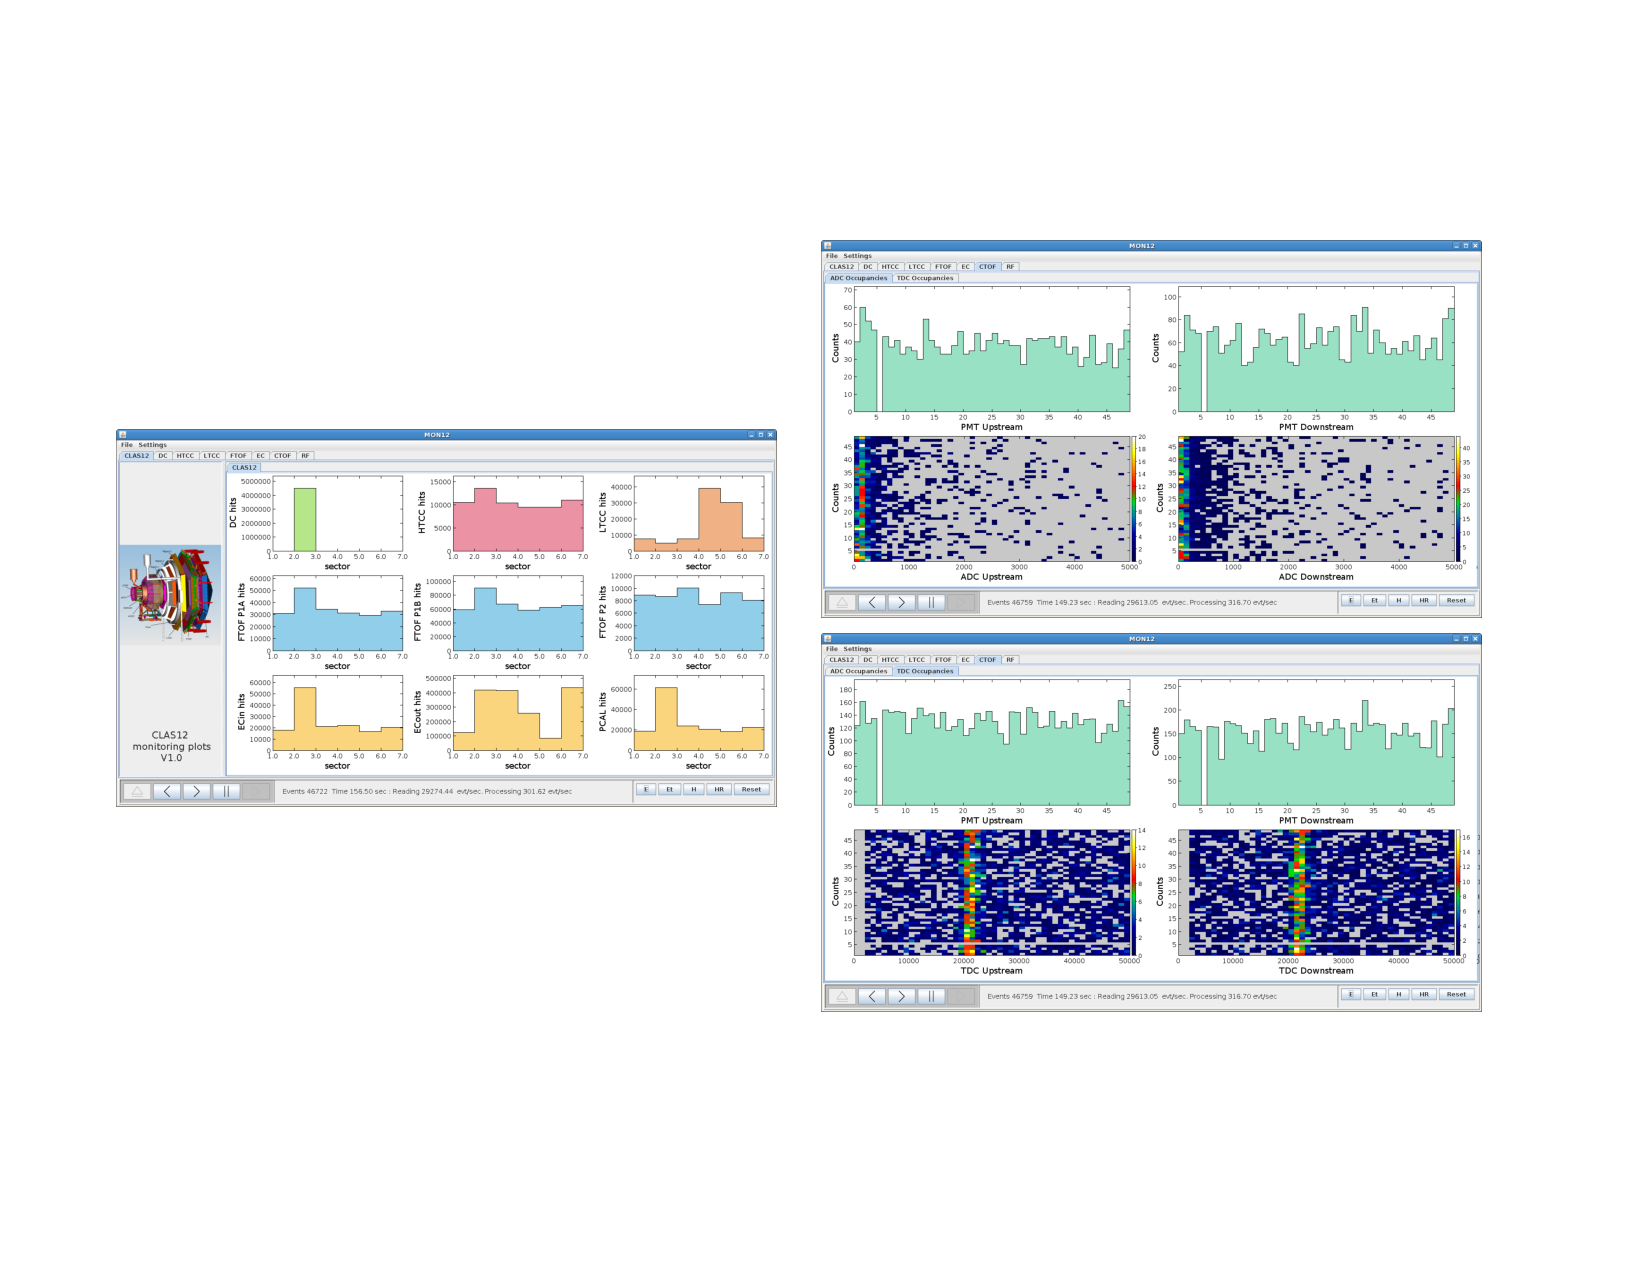
\includegraphics[width=0.80\textwidth,natwidth=610,natheight=642]{mon12.pdf}}}
\end{picture} 
\caption{(Left) The main {\it mon12} display screen showing counts across the 
different CLAS12 subsystems and sectors. (Right) The CTOF ADC and TDC scaler screens 
within {\it mon12}.}
\label{mon12}
\end{figure}
%%%%%%%%%%%%%%%%%%%%%%%%%%%%%%%%%%%%%%%%%%%%%%%%%%%%%%%%%%%%%%%%%%%%%%%%%%%%%%%%%%%

The {\it mon12} utility requires the data acquisition system to be operating to 
display the scaler counts. If a run is in progress, scaler accumulation will begin 
by selecting the event source (either the ET or HIPO rings or EVIO or HIPO data 
files in the lower right of the screen) and then clicking on the ``play'' button 
(the rightward triangle in the lower left of the screen). The CTOF scalers are
available for both the FADC and TDC channels by clicking on the CTOF tab and
selecting either sub-tab ``ADC Occupancies'' or ``TDC Occupancies'' as shown in
Fig.~\ref{mon12}(right).

\vfil
\eject

%%%%%%%%%%%%%%%%%%%%%%%%%%%%%%%%%%%%%%%%%%%%%%%%%%%%%%%%%%%%%%%%%%%%%%%%%%%%%%%%%%%
\begin{figure}[ht]
\vspace{7.0cm}
\begin{picture}(30,50) 
\put(10,-35)
{\hbox{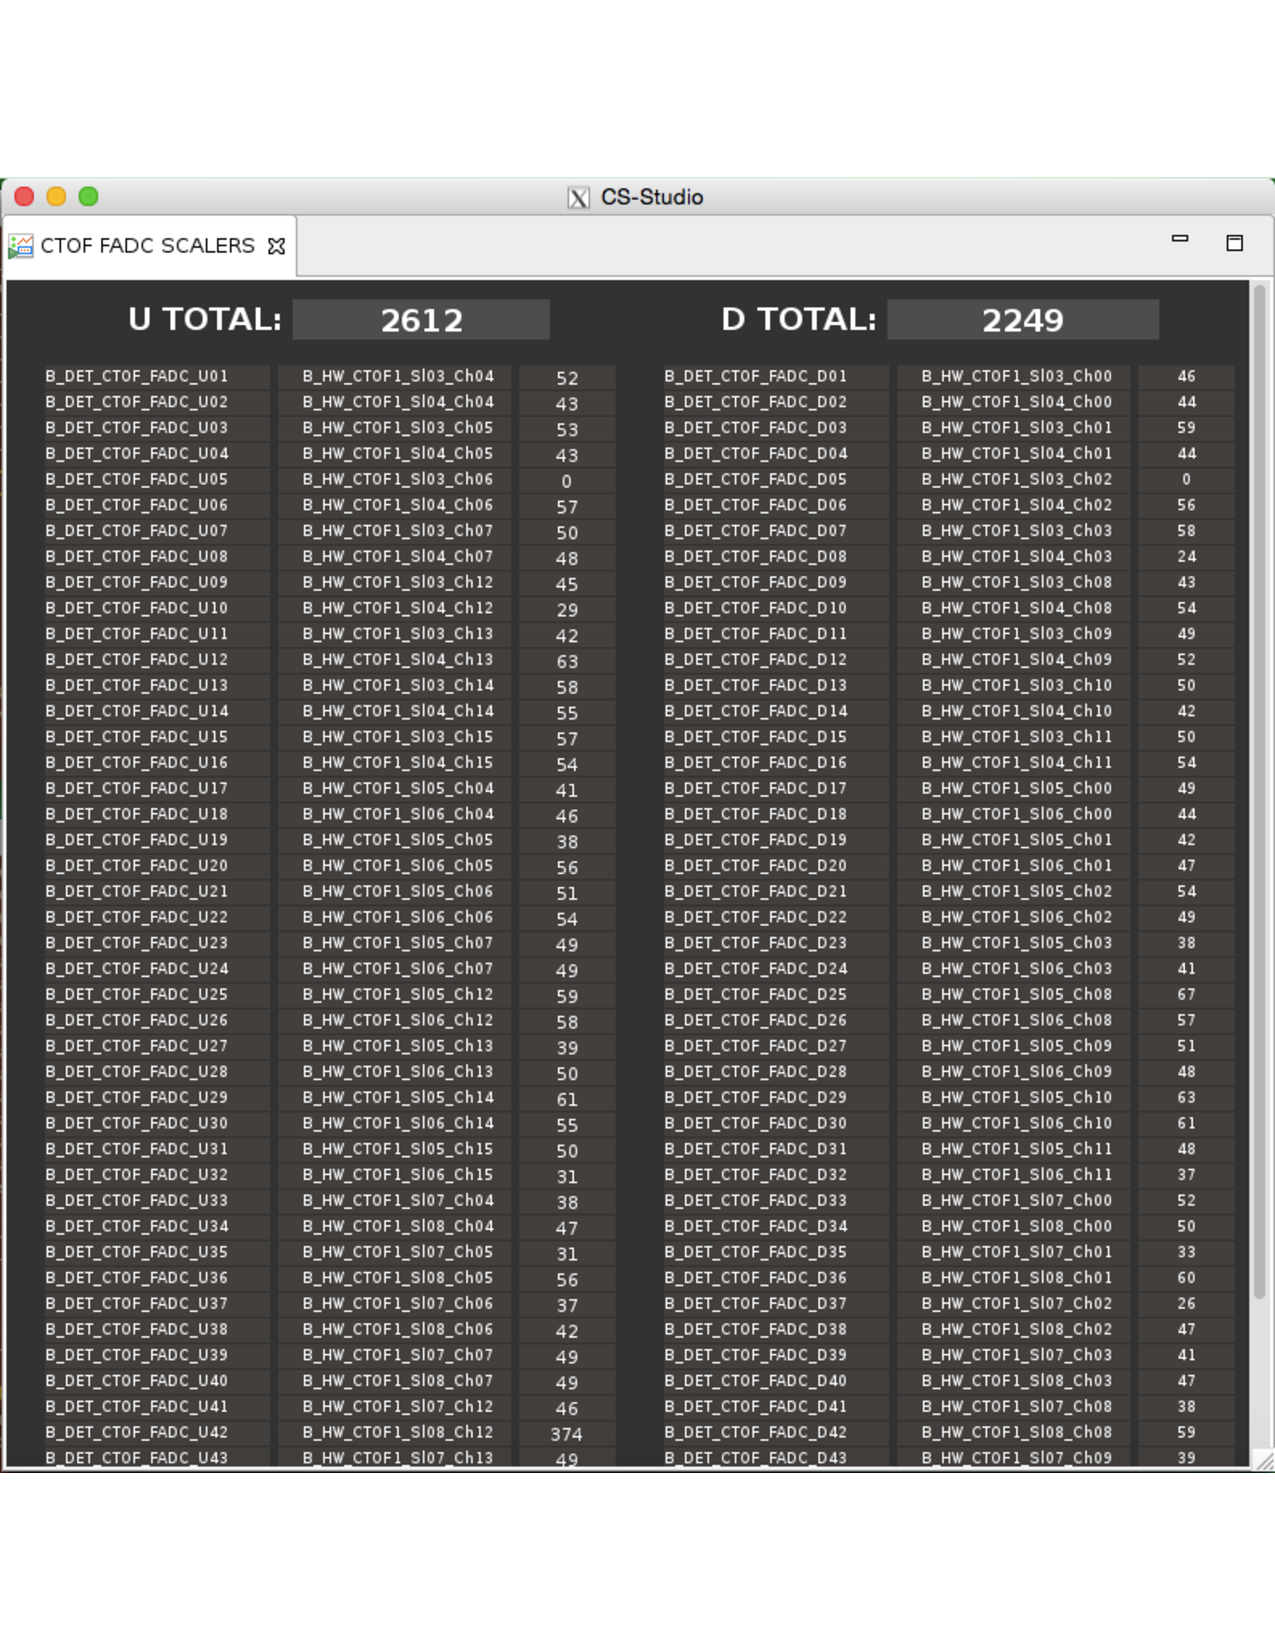
\includegraphics[width=0.50\textwidth,natwidth=610,natheight=642]
{scaler-screen-ctof.pdf}}}
\put(245,-35)
{\hbox{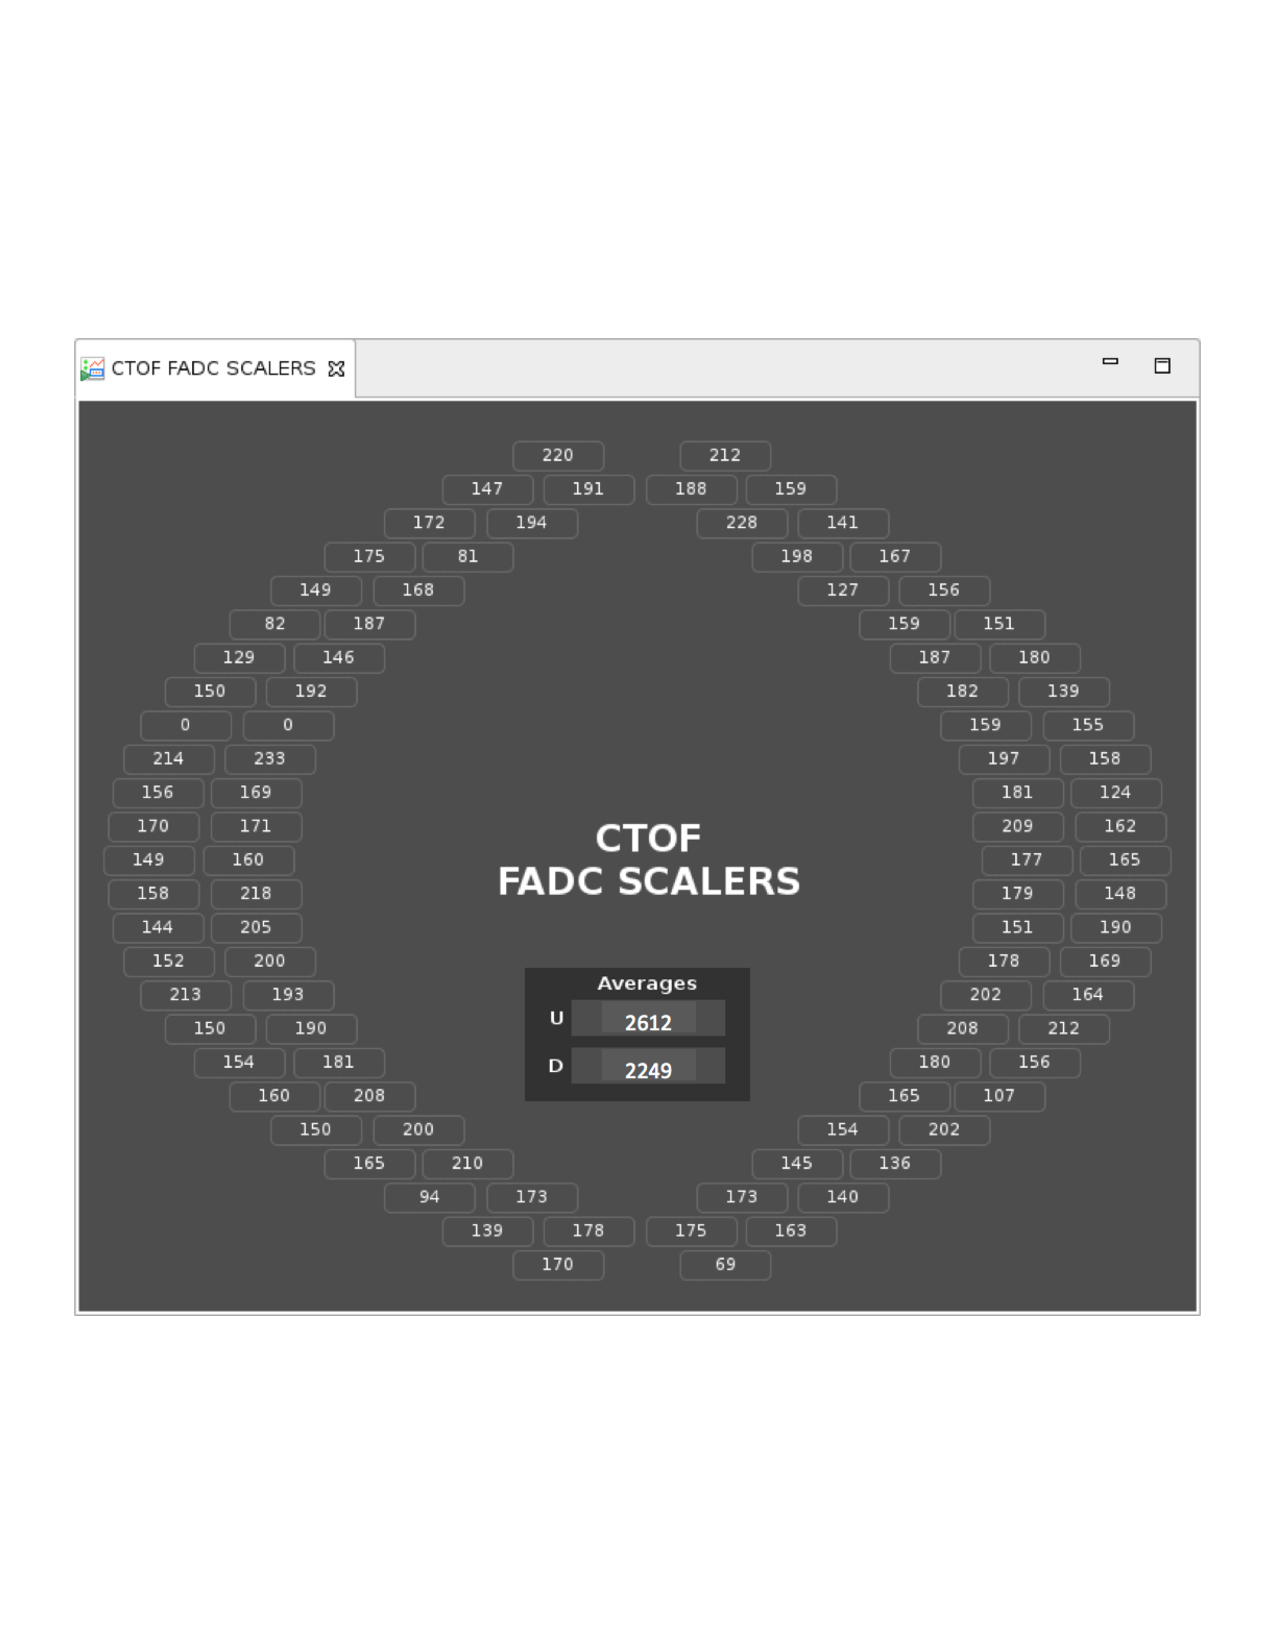
\includegraphics[width=0.50\textwidth,natwidth=610,natheight=642]
{scaler-screen2-ctof.pdf}}}
\end{picture} 
\caption{Scaler displays for the CTOF counters from the Slow Controls system
showing the two different options, ``CTOF Scalers'' (left) and ``CTOF Scalers -
Geographic'' (right). Both displays show the total rate for the upstream and 
downstream PMTs.}
\label{sc-scalers}
\end{figure}
%%%%%%%%%%%%%%%%%%%%%%%%%%%%%%%%%%%%%%%%%%%%%%%%%%%%%%%%%%%%%%%%%%%%%%%%%%%%%%%%%%%

The second manner in which to view the CTOF system scalers is through the CLAS12 
Slow Controls system. Shown in the options for the CTOF system in 
Fig.~\ref{ctof-screen1-2}(right) is an option to view the CTOF scalers from the
FADCs. Note that there are presently two different options for displaying the
same information, ``CTOF Scalers'' and ``CTOF Scalers - Geographic''. Selecting 
these options brings up the screens as shown in Fig.~\ref{sc-scalers}.

The final manner in which to monitor the performance of the CTOF hardware is
through the expert monitoring suite {\it CTOFMON}. Details on this suite are
provided in Section~\ref{ctofmon}, however this suite is mainly intended for
CTOF system experts.

\clearpage

\vfil
\eject

\section{Information for Subsystem Experts}

\subsection{Subsystem Expert Responsibilities}

The CTOF subsystem experts have several key responsibilities:

\begin{enumerate}
\item Complete hot checkout sign-off before the start of each run period (see 
Section~\ref{checkout}).
\item Respond to calls on the on-call phone to resolve issues with the CTOF system 
during data taking (see Section~\ref{oncall}).
\item Take periodic HV gain calibration runs and adjust the system HV settings (see 
Section~\ref{gain-calib}).
\item Take periodic LMS performance runs (see Section~\ref{lms-scans}).
\item Monitor the system performance with the {\it CTOFMON} expert monitoring suite
(see Section~\ref{ctofmon}).
\item Make repairs to the hardware during maintenance periods (see 
Section~\ref{repairs}).
\end{enumerate}

\subsubsection{Hot Checkout}
\label{checkout}

Prior to the start of each beam running period, each subsystem Group Leader is 
responsible to review the components of their systems to be sure that they are 
fully operational. This review is referred to as ``hot checkout''. The hot checkout 
is an online checklist for each subsystem that includes a sign-off for all hardware 
elements of the system (e.g. HV, LV, detectors, gas, pulser). For the CTOF system, 
the hot checkout includes verification that all detectors are operational, that the 
Slow Controls system for the HV and LMS is functioning, and that the DAQ system can 
fully communicate with the readout electronics. It also includes checkout that the 
LV power supply system and the shield temperature readout are operational. 

Fig.~\ref{hot-co} shows a screenshot of the hot checkout interface. Under the heading 
``Hall~B CLAS12 Detector'', all entries for CTOF (located within the ``CLAS12 TOF''
subheading) must be verified as ready. Note that often as part of the system checkout 
before the start of a run period, an initial HV gain calibration is completed (see 
Section~\ref{gain-calib}) and an LMS performance scan is taken (see 
Section~\ref{lms-scans}). Reminders to complete the system hot checkout will be sent 
out shortly before the start of a given run period with the required deadline for 
completing the work.

%%%%%%%%%%%%%%%%%%%%%%%%%%%%%%%%%%%%%%%%%%%%%%%%%%%%%%%%%%%%%%%%%%%%%%%%%%%%%%%%%%%
\begin{figure}[ht]
\vspace{9.5cm}
\begin{picture}(30,50) 
\put(35,-5)
{\hbox{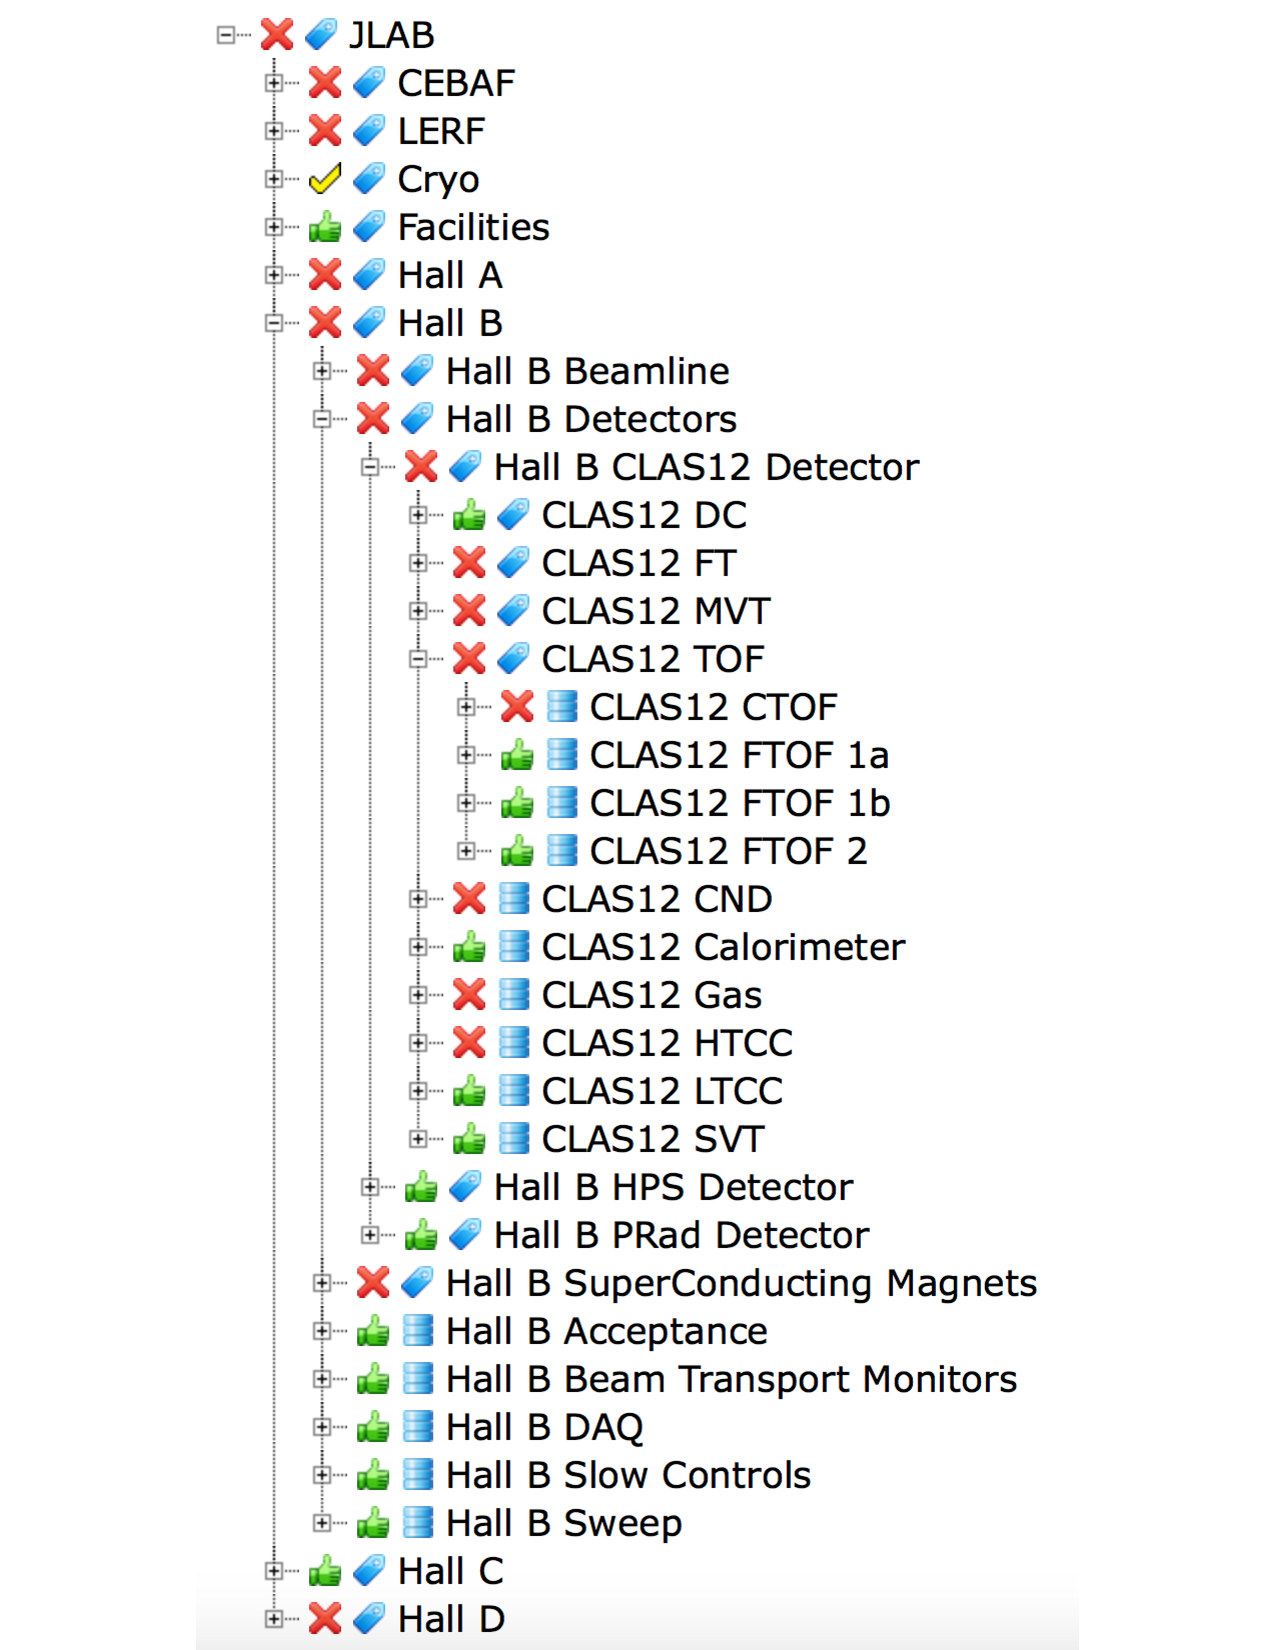
\includegraphics[width=0.55\textwidth,natwidth=610,natheight=642]
{checklist1.pdf}}}
\put(270,40)
{\hbox{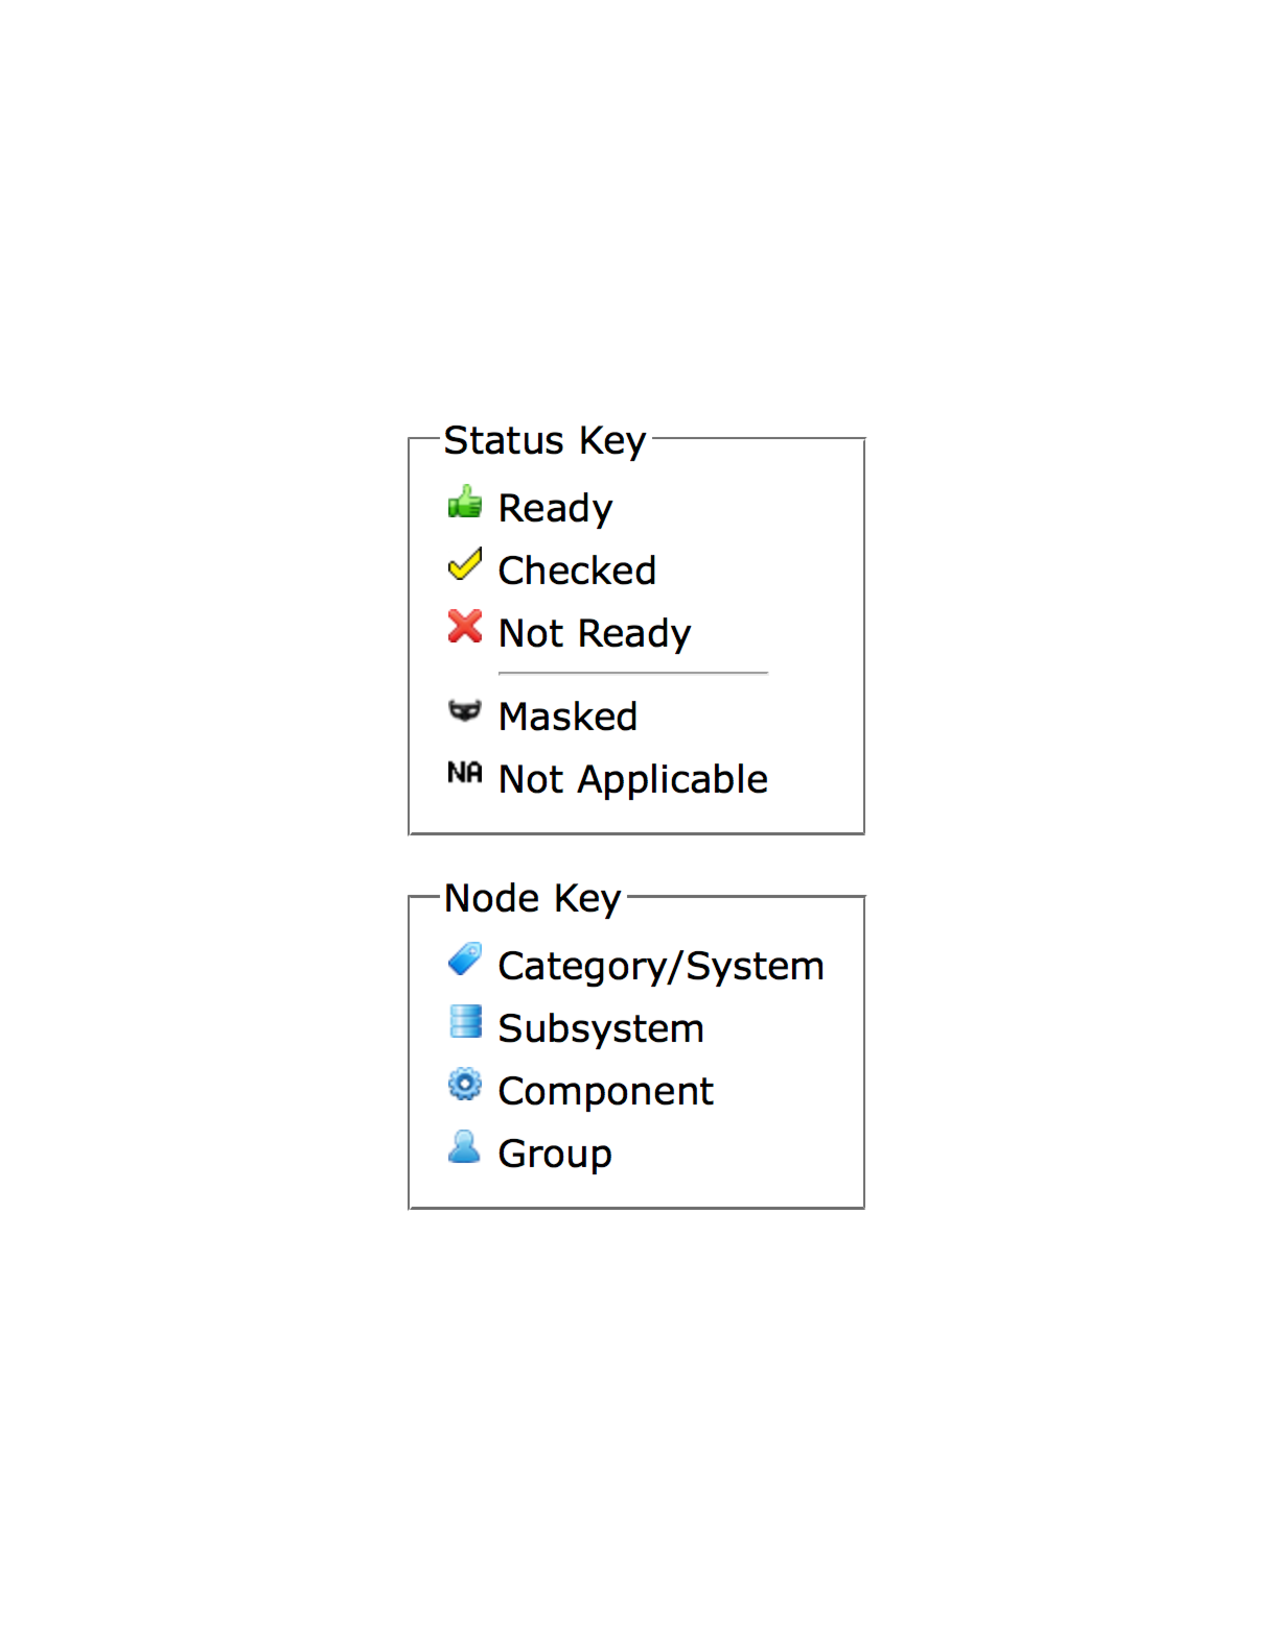
\includegraphics[width=0.35\textwidth,natwidth=610,natheight=642]
{checklist2.pdf}}}
\end{picture} 
\caption{Screenshot of the Hall~B hot checkout screen. The CTOF system appears under 
the ``Hall~B CLAS12 Detector'' and ``CLAS TOF'' headings. All entries for CTOF have 
to be verified as functional and all items listed as ``Not Ready'' must be changed 
over to ``Ready''.}
\label{hot-co}
\end{figure}
%%%%%%%%%%%%%%%%%%%%%%%%%%%%%%%%%%%%%%%%%%%%%%%%%%%%%%%%%%%%%%%%%%%%%%%%%%%%%%%%%%%

\subsubsection{On-Call Responsibilities}
\label{oncall}

Each subsystem Group Leader will organize a list of on-call experts who will 
take responsibility for carrying a cell phone to allow 24~hour access to experts 
who can address any problems that arise during a beam running period. The 
phone numbers of all subsystem experts are posted on the run page~\cite{run-page}. 
Any problems that cannot be quickly solved by the shift workers, where quickly 
amounts to 10 to 15~minutes, should result in a call to the relevant expert cell 
phone. \textcolor{red}{The CTOF on-call phone number is (757)-344-7204.} 

The on-call experts can often diagnose problems over the telephone, but there are 
times where they will have to go to the Counting House to more fully address an 
issue. One of the important responsibilities of the on-call experts is to make 
practical decisions regarding which problems require access to Hall~B for immediate 
attention and which can be delayed to periods when the accelerator is down or other 
work is scheduled in the hall. For the CTOF system, usually problems with a single 
channel are not important enough to stop the data acquisition. The normal mode of 
operation after initial investigation of a bad channel is to turn off the HV for 
that channel until access can be made for a more detailed investigation. This work 
should be coordinated with the Run Coordinator. Access to PMTs for service must be 
done only when the solenoid is off.

Note: It is the responsibility of the CTOF on-call expert to review all issues that 
they cannot resolve with the CTOF subsystem Group Leader as soon as is reasonable.

\subsubsection{HV Gain Calibrations}
\label{gain-calib}

The HV gain calibrations for the CTOF system are typically completed before the 
start of each run period, as well as several times during the run period when there 
is opportunity. The HV gain calibration procedure employs a cosmic ray trigger 
defined by the CTOF system. The ADC spectra for each counter are fit to determine
the minimum ionizing particle peak position. The end result of the gain calibration 
amounts to adjusting the system HV settings to position the ADC peaks at their 
assigned locations corresponding to a specific PMT gain.

The calibration suite for the CTOF system is used to calibrate the PMT gains and 
the output is a table of PMT HV settings in the appropriate file format that are 
downloaded into the HV power supplies. This calibration suite is also used to 
determine the parameters to optimize the timing resolution of the system. Full 
documentation on using the CTOF calibration suite, including a tutorial for using 
the code, is included on the CTOF web page~\cite{ctof-web}.

\subsubsection{LMS Scans}
\label{lms-scans}

The CTOF Light Monitoring System (LMS) consists of an optical fiber coupled to 
the light guide near each PMT. The light source is an LED board that is driven by 
a JLab-designed VME pulser board~\cite{pulser-board}. The LED source is coupled to 
the fiber array through a small focusing Acrylic light guide.

%%%%%%%%%%%%%%%%%%%%%%%%%%%%%%%%%%%%%%%%%%%%%%%%%%%%%%%%%%%%%%%%%%%%%%%%%%%%%%%%%%%
\begin{figure}[htbp]
\vspace{9.0cm}
\begin{picture}(30,50) 
\put(120,-3)
{\hbox{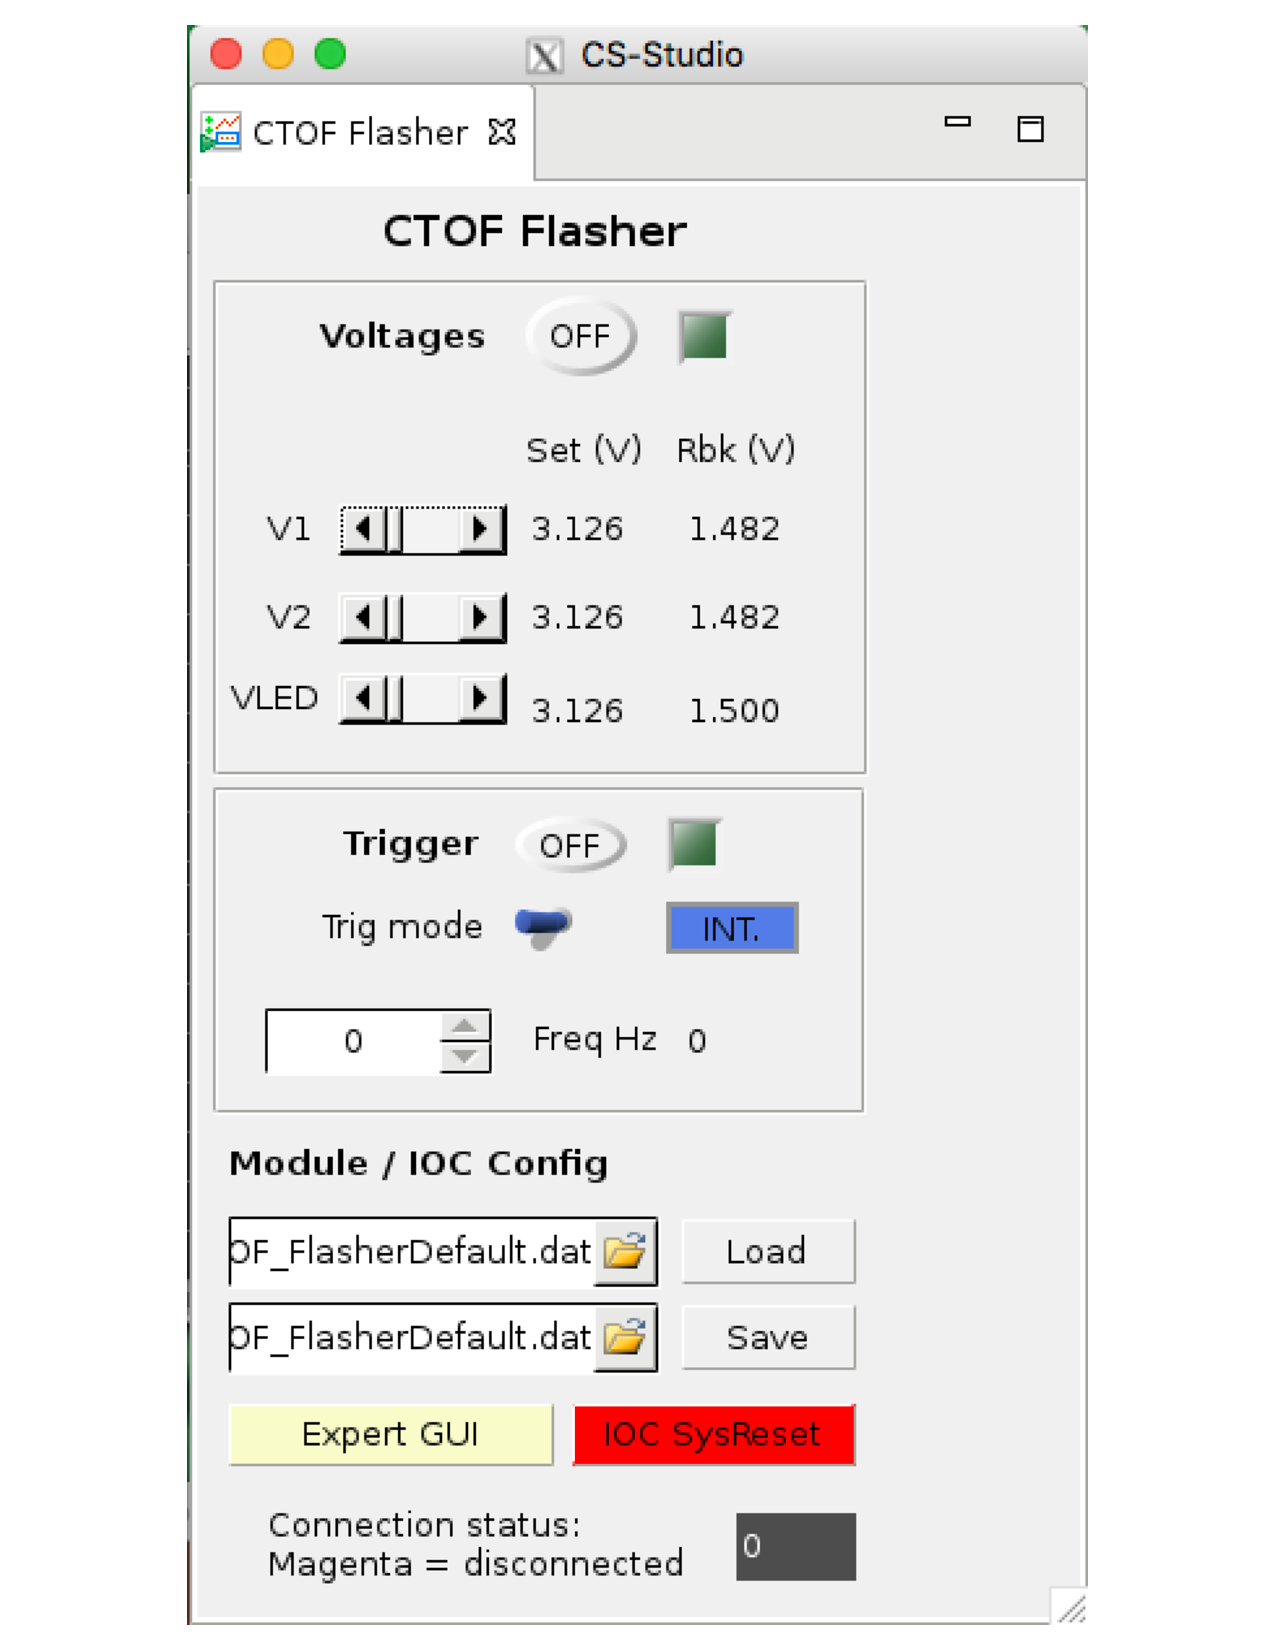
\includegraphics[width=0.50\textwidth,natwidth=610,natheight=642]
{ctof-lms.pdf}}}
\end{picture} 
\caption{Pulser control interface screen for the CTOF LMS.}
\label{ctof-lms}
\end{figure}
%%%%%%%%%%%%%%%%%%%%%%%%%%%%%%%%%%%%%%%%%%%%%%%%%%%%%%%%%%%%%%%%%%%%%%%%%%%%%%%%%%%

The LMS scan sequence amounts to taking six separate data runs adjusting the LED 
light amplitude in discrete increments to vary the intensity over the full dynamic 
range of the FADC. This interface is brought up by clicking on the ``CTOF LMS'' 
option from the CTOF sub-menu shown in Fig.~\ref{ctof-screen1-2}. Note that the 
pulser board has two outputs, one for the CTOF system and one for the HTCC system. 
Fig.~\ref{ctof-lms} shows a preliminary version of the control interface that is 
still being worked on. The intensity scan is controlled by adjusted VLED from 
3.5~V to 6.0~V in 0.5~V steps. The nominal pulser frequency for the scan is 1~kHz. 
Problems with communication between the LMS controls and the pulser board are 
indicated by a magenta color on the interface. If these are present, that is an 
indication that the associated pulser IOC needs to be rebooted (see 
Section~\ref{reset-iocs}). Contact the Slow Controls expert if there are any
communication problems that are not remedied after an IOC reboot.

\subsubsection{Expert Monitoring Suite}
\label{ctofmon}

The expert monitoring suite for the CTOF system is called {\it CTOFMON}. This code 
suite is brought up on any Counting House computer by typing ``ctofmon''. The suite 
allows monitoring of the following system quantities:

\begin{itemize}
\item FADC Mode 1 time slices
\item Channel ADCs and TDCs
\item Pedestal centroids and widths
\item MIP responses
\item HV settings
\item Scalers
\end{itemize}

The suite runs from EVIO or HIPO input files or by attaching directly to the DAQ 
ET ring. The suite can also read and display input histogram files. Screen captures 
of the suite are shown in Fig.~\ref{ctofmon-screens}. 

%%%%%%%%%%%%%%%%%%%%%%%%%%%%%%%%%%%%%%%%%%%%%%%%%%%%%%%%%%%%%%%%%%%%%%%%%%%%%%%%%%%
\begin{figure}[htbp]
\vspace{15.0cm}
\begin{picture}(30,50) 
\put(40,560)
{\hbox{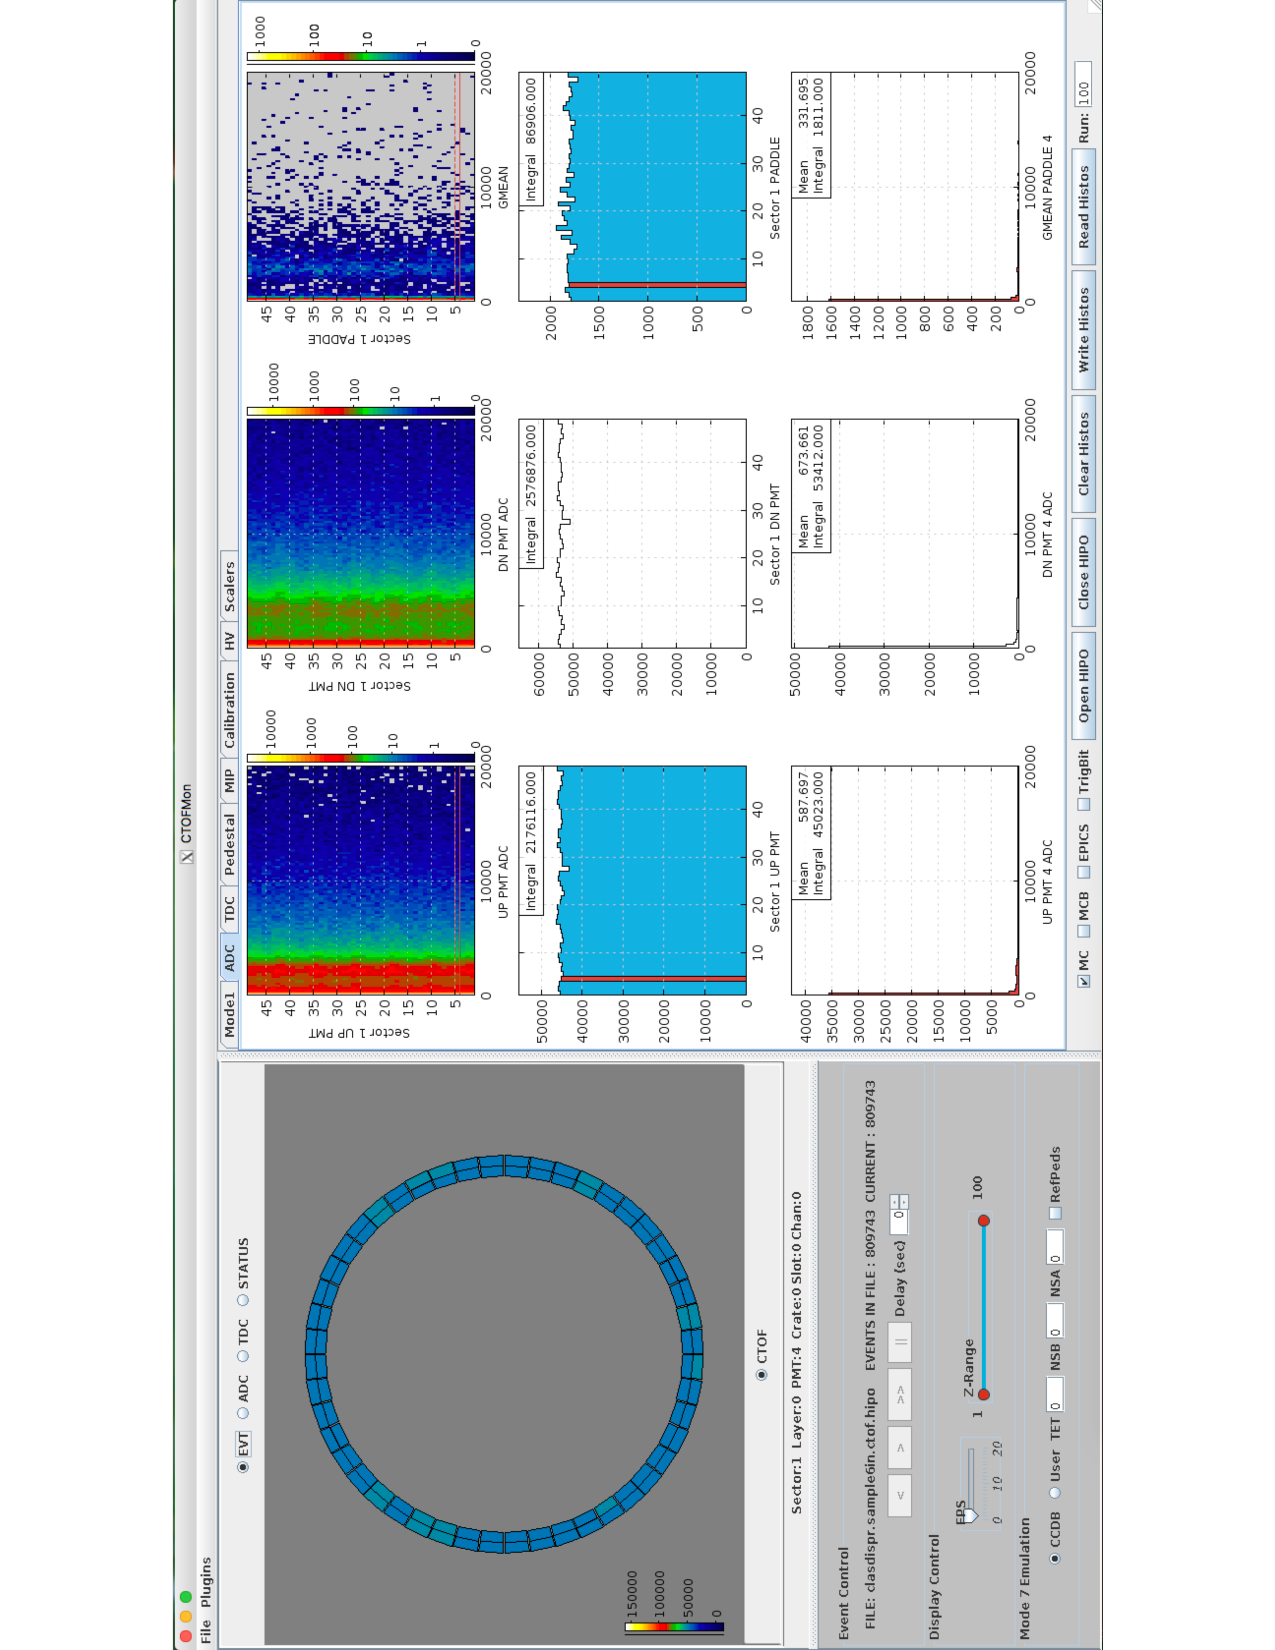
\includegraphics[width=0.70\textwidth,natwidth=610,height=0.50\textheight,
natheight=642,angle=-90]{ctofmon-1.pdf}}}
\put(40,300)
{\hbox{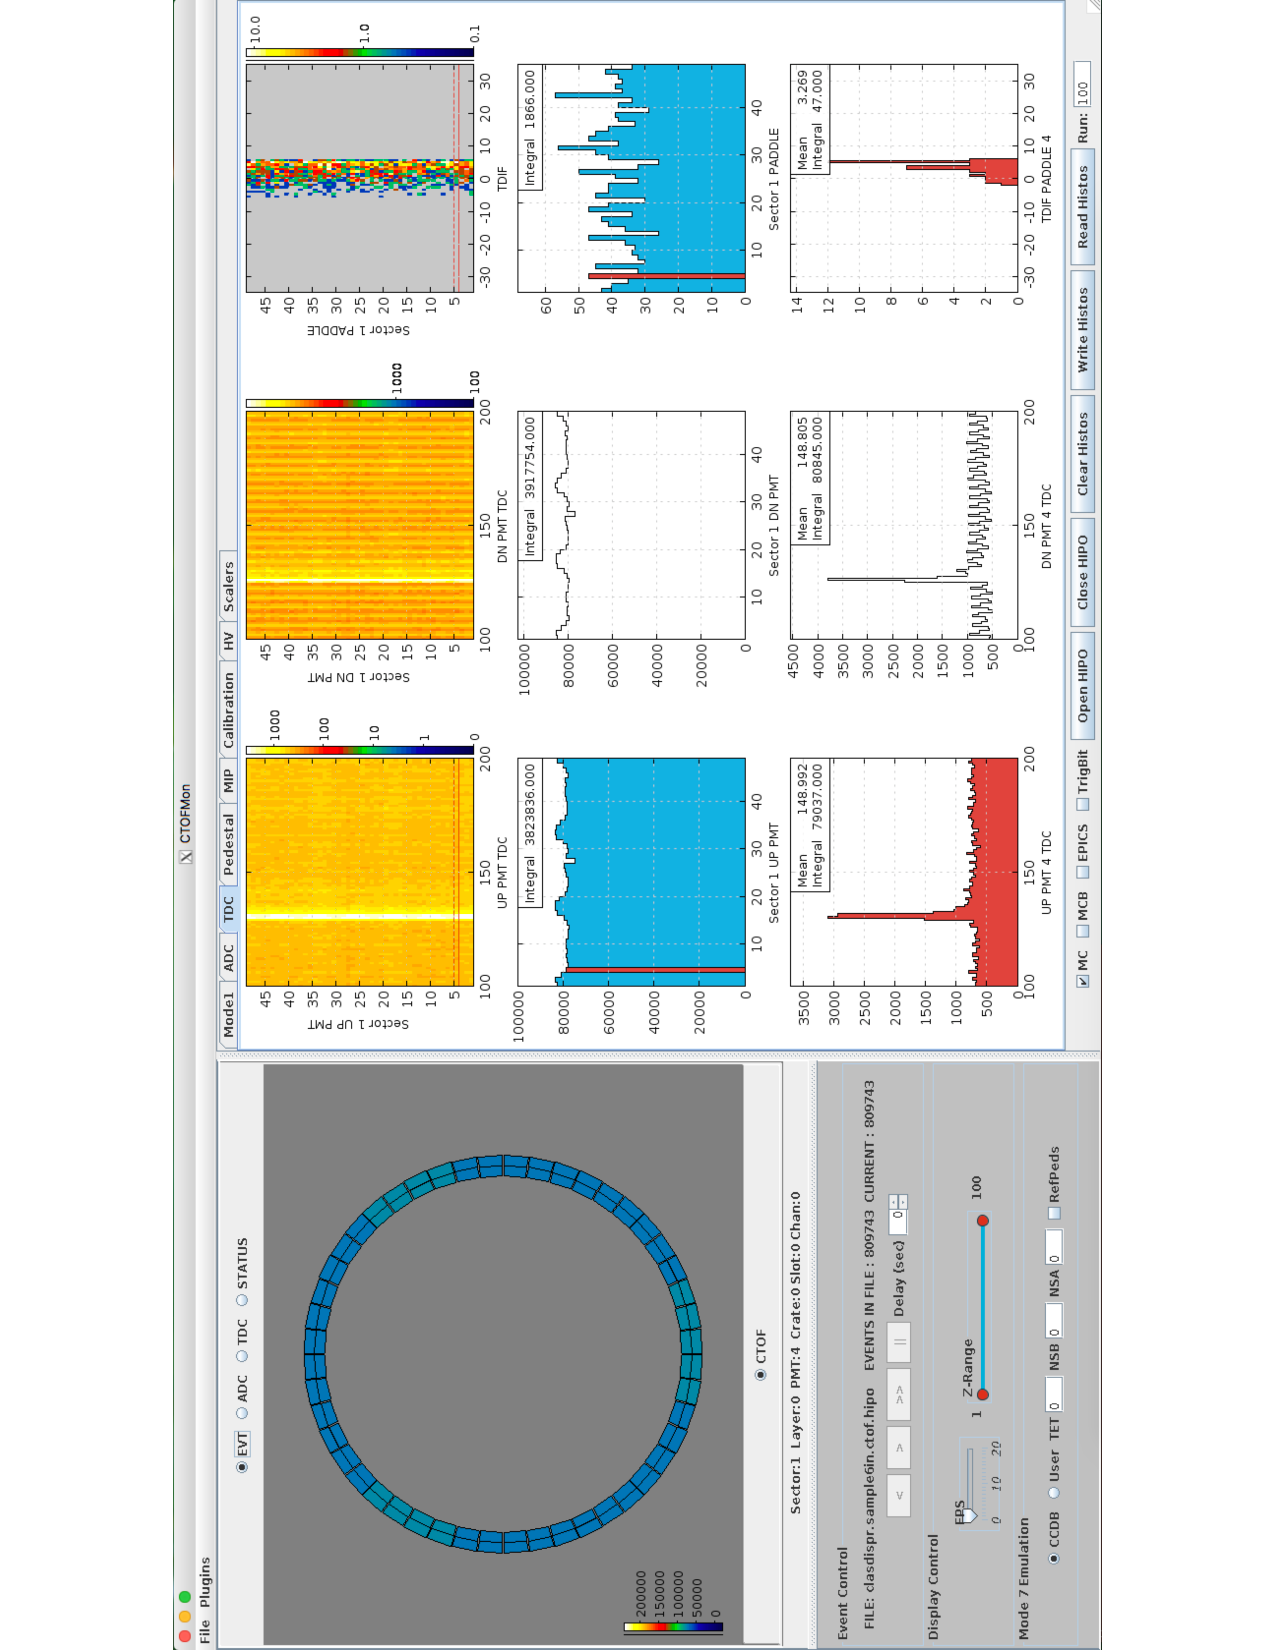
\includegraphics[width=0.70\textwidth,natwidth=610,height=0.50\textheight,
natheight=642,angle=-90]{ctofmon-2.pdf}}}
\end{picture} 
\caption{Screens from the {\it CTOFMON} expert monitoring suite.}
\label{ctofmon-screens}
\end{figure}
%%%%%%%%%%%%%%%%%%%%%%%%%%%%%%%%%%%%%%%%%%%%%%%%%%%%%%%%%%%%%%%%%%%%%%%%%%%%%%%%%%%

\subsection{System Failure Modes}
\label{repairs}

For the CTOF detector, there are a number of usual ``failure'' modes with which the 
system expert should be familiar. These include the following:

\begin{itemize}
\item Bad HV board (see Section~\ref{board-swap})
\item Bad HV mainframe (see Section~\ref{mainframe})
\item Sudden ADC gain shift (see Section~\ref{gain-shift})
\item High PMT dark current (see Section~\ref{high-current})
\item Missing or bad signal (see Section~\ref{missing})
\item Bad PMT (see Section~\ref{bad-pmt})
\item Readout electronics issues (see Section~\ref{readout-issues})
\item IOC issues (see Section~\ref{ioc-issues})
\end{itemize}

\subsubsection{Bad HV Board}
\label{board-swap}

The evidence for a bad HV board (A1535N) is either that the 24 channels associated 
with a single board won't ramp up to full voltage before tripping off or bad voltage 
regulation. For the case of bad voltage regulation, the channels ramp up to full 
voltage but then fluctuate about the demand voltage setting by up to several hundred 
volts. Before deciding whether a HV board is bad, some investigation should be 
completed to ensure that a single HV channel is not causing the problems with the 
board, which could point to a problem with the PMT or voltage divider. If a board is 
deemed bad and needs to be replaced, the following steps are necessary:

\begin{enumerate}
\item Using the HV control interface, ensure that all HV channels controlled by the
mainframe are turned off. Remember that the HV mainframe for the CTOF also includes 
the HTCC and some beamline devices.
\item Take a spare A1535N board from the storage area on the second level of the Pie 
Tower in Hall~B.
\item Turn the front panel key on the HV supply to the ``off'' position and toggle 
the main power switch to ``off'' on the back of the HV supply.
\item On the back of the supply, remove the Radiall connector on the bad board.
\item Pull out the bad board, being careful of the Radiall connectors on the 
neighboring boards.
\item Install the new board and reconnect the Radiall connector.
\item Be sure to take out the 50~$\Omega$ lemo interlock terminator from the old 
board and plug into the same connector on the new board.
\item Toggle the main power switch to ``on'' and turn the HV power supply on using 
the key on the front panel, putting the key in the ``local'' position.
\item Run all parameter scripts for the HV power supply to load all channel 
parameters. See instructions in Section~\ref{hv-parms}. Note that only the parameters
associated with the newly installed board should need to be set.
\item Enter information on the new board and the old bad board into the Hall~B 
equipment database (see the Appendix).
\item Leave the bad board on the RadCon Survey table in Hall~B.
\item If beam conditions are acceptable, turn on the HV for the CTOF, HTCC, and
beamline device channels. Be sure to check with the shift leader before energizing 
the supply.
\end{enumerate}

\subsubsection{Bad Mainframe}
\label{mainframe}

From time to time the CAEN mainframes will go bad and need to be serviced in situ or
replaced entirely with a spare. If the entire mainframe must be replaced, this can be
a fairly significant undertaking and should not be considered without certainty that 
the problem is actually the mainframe. The final determination regarding the status 
of the hardware should be made in consultation with the Slow Controls expert after a 
number of different checks are made.

The basic procedure to swap out a mainframe is as follows:

\begin{enumerate}
\item Using the HV control interface, ensure that all HV channels controlled by the
mainframe are turned off. Remember that the HV mainframe for the CTOF also includes 
the HTCC and some beamline devices.
\item Turn the front panel key on the HV supply to the ``off'' position and toggle 
the main power switch to ``off'' on the back of the HV supply.
\item The modules are typically pulled out of the back of the mainframe leaving the 
Radiall connectors attached. Before pulling the modules from the mainframe, be sure 
that they are clearly labeled so that they can be put back into their assigned channels.
\item Unplug the power cord from the mainframe.
\item Remove the mainframe from the rack and place it on the radiation survey table. 
Send email to the Fast Electronics Group to pick up the mainframe for testing/repairs.
\item Install a spare mainframe in the rack, install the boards into their assigned 
slots, and connect the power cord to the mainframe.
\item Toggle the main power switch to ``on'' and turn the HV power supply on using the 
key on the front panel, putting the key in the ``local'' position.
\item Contact the Slow Controls expert to set up communication to the mainframe.
\item When communication is restored, check the channel settings for all boards to be 
sure that they are correct before turning on the HV. If there are questions regarding 
the HTCC settings, contact the HTCC expert. If there are questions regarding the
beamline device settings, contact the beamline expert.
\item If beam conditions are acceptable, turn on the HV for the CTOF, HTCC, and
beamline device channels. Be sure to check with the shift leader before energizing 
the supply.
\end{enumerate}

\subsubsection{Sudden Gain Shift}
\label{gain-shift}

Sometimes a sudden gain shift can appear in the ADC spectra for a given counter. 
There are a number of possible causes for such a condition.

\begin{itemize}
\item Problematic PMT - sometimes gain shifts can be attributed to a problem with a 
PMT that requires adjustment of the HV settings. Of course, PMT gain issues typically 
lead to a reduced gain that requires an increase of the HV.  Such issues are typically 
seen as slow drifts of the response with time.
\item DAQ Problems - the most common cause for an apparent gain shift in the ADC 
spectra for a counter is due to problems with the FADC settings. Such problems can 
typically be diagnosed from pedestal shifts or widened pedestals. The pedestals can be 
checked by taking FADC data in ``raw mode'' using the {\it CTOFMON} system monitoring 
suite (see Section~\ref{ctofmon}).
\item Light Leak - it is possible that a gain shift can be due to a light leak on the 
counter. The detectors themselves can be checked as necessary, coordinating work 
through the Run Coordinator and the Hall~B Work Coordinator.
\item PMT Saturation - In conditions of excessive high rate, the PMT becomes current 
limited and the ADC signals can become distorted and shifted to lower gains. Be sure 
that bad beam or high rate conditions are not responsible for the issues seen.
\end{itemize}

\subsubsection{High PMT Dark Current}
\label{high-current}

High PMT dark currents can be seen through increased counting rates in the channel 
scaler displays or in distorted ADC spectra. The dark currents can be measured at 
either the splitter boxes (nominal measurement location) or at the PMT output (if 
the solenoid is off). There are two likely causes for high PMT dark currents:

\begin{enumerate}
\item Bad PMT - At times when a PMT goes bad, its dark current can increase. Typical 
CTOF PMT dark currents are at the level of 50~nA or less. If a bad PMT has been 
identified, it can be replaced during a scheduled Hall~B access. However, the usual 
procedure is to leave the PMT energized and live with the increased dark current 
unless the higher currents cause the HV supply channel to trip or the HV board to
become unstable. If the channel HV needs to be ``turned off'', change $V_{set}$=0. 
The logbook should be updated and the HV setting configuration with the channel off 
should be saved as the nominal setting.
\item Light Leak - A light leak in the counter wrapping can also lead to higher dark 
currents. The issue of light leaks is not expected to be an issue on the scintillation 
bars as they are buried within the solenoid and ambient light levels are usually very 
low. However, the long upstream and downstream light guides are more exposed. Light 
leaks can be investigated and repaired during a scheduled Hall~B access.
\end{enumerate}

\subsubsection{Missing or Bad Signal}
\label{missing}

Each CTOF PMT has a single anode signal output. This signal is a negative polarity 
pulse as shown in Fig.~\ref{pmt-pulses} for a representative pulse from one of the 
counters.

%%%%%%%%%%%%%%%%%%%%%%%%%%%%%%%%%%%%%%%%%%%%%%%%%%%%%%%%%%%%%%%%%%%%%%%%%%%%%%%%%%%
\begin{figure}[htbp]
\vspace{5.2cm}
\begin{picture}(30,50) 
\put(65,230)
{\hbox{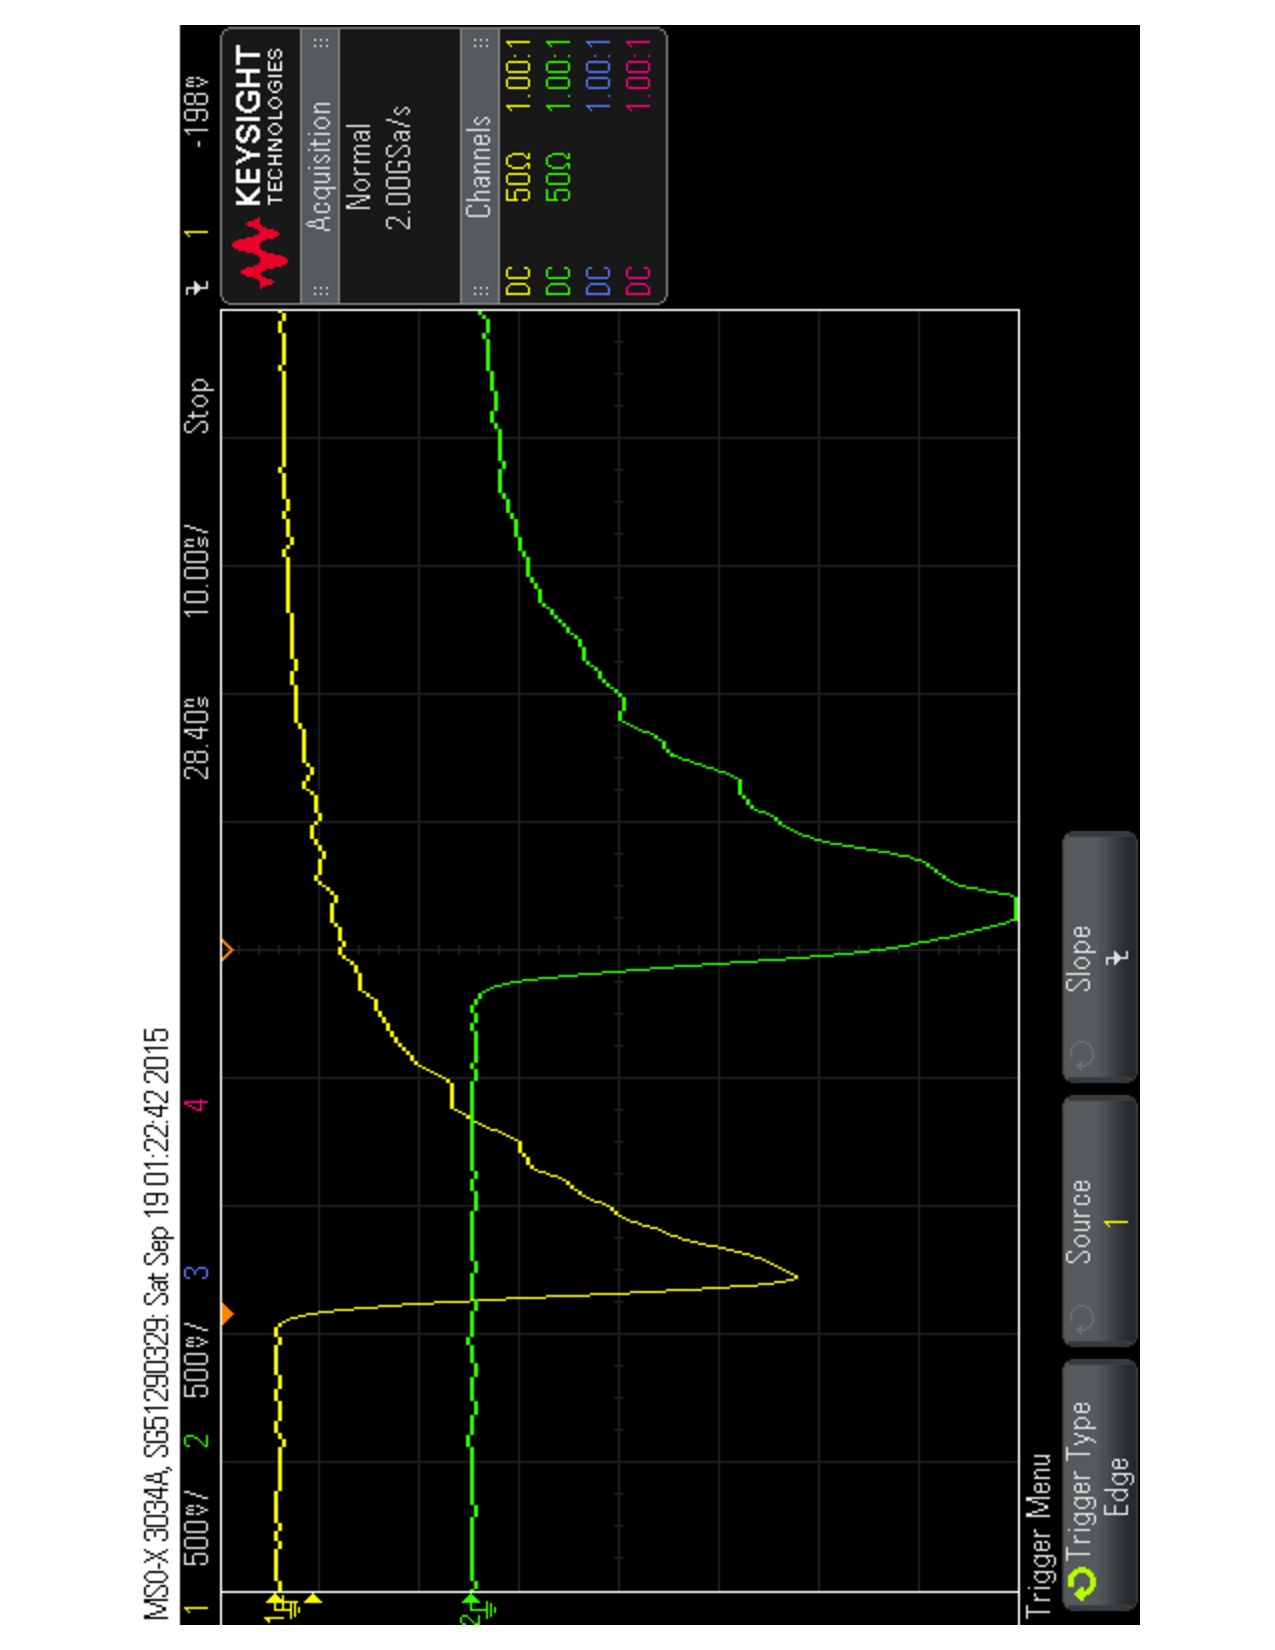
\includegraphics[width=0.55\textwidth,natwidth=610,natheight=642,angle=-90]
{scope.pdf}}}
\end{picture} 
\caption{Scope traces of a representative anode pulse for the upstream and 
downstream PMTs of a CTOF counter.}
\label{pmt-pulses}
\end{figure}
%%%%%%%%%%%%%%%%%%%%%%%%%%%%%%%%%%%%%%%%%%%%%%%%%%%%%%%%%%%%%%%%%%%%%%%%%%%%%%%%%%%

Occasionally a signal channel will disappear from the CTOF monitoring plots. In such a 
situation, further investigation will be necessary. 

\begin{itemize}
\item If a signal channel is missing, this could be due either to a problem with 
the HV, the VME crate (which would affect and entire board), or the PMT itself. If 
the problem is with the HV board, it should be replaced as detailed in 
Section~\ref{board-swap}. PMT problems are typically apparent as the nominal PMT 
signal is absent, severely distorted, or replaced by high frequency noise.
\item If a signal channel is missing, this could be a bad cable connection anywhere 
from the voltage divider to the input to the electronics. The way to diagnose is to 
use an oscilloscope to look at the signal at each accessible junction point. If the 
signal is missing from the monitoring data but is seen to be good at the input to 
the FADC and TDC, contact the DAQ expert for help.
\item A common reason why a PMT signal is seen to have a high frequency noise 
component (called ringing) is due to a loose signal cable connector associated with 
the RG-174 or RG-316 cables. In such a case ensure that the connector barrel is 
screwed on tightly to the connector threads.
\item If the PMT HV is on but the supply current reads 0, this is likely due to a bad 
HV cable or connection, or an issue with the HV distribution box.
\item Groups of missing signals for consecutive electronics channels are likely due to 
an unplugged or partially unplugged ribbon cable at the input to the TDCs.
\end{itemize}

\subsubsection{Bad PMT}
\label{bad-pmt}

One of the most common failure modes of a PMT is a gradual loss of gain over the 
period of several years. This can be compensated by adjusting the HV to maintain 
the gain setting. The PMTs used in the CTOF system have a maximum voltage rating 
of -2500~V. Once the PMT HV is set to its maximum value and the gain falls below 
the nominal setting, the PMT should be flagged for replacement during the next 
servicing opportunity. Note that the serial numbers for the removed and replacement 
PMTs should be recorded in the CTOF PMT database. The removed PMTs should be
cleared by survey and given to the CTOF Group Leader for further evaluation.

\subsubsection{Readout Electronics Issues}
\label{readout-issues}

Readout electronics issues, typically associated with all channels associated with 
a given discriminator module, TDC board, or FADC board, once diagnosed should be 
brought to the attention of the DAQ system expert for further diagnosis and attention.

\subsubsection{IOC Issues}
\label{ioc-issues}

Loss of communication between the IOC and the HV mainframe is seen by a yellow or
magenta color status for the HV channels on the CTOF HV display (see 
Section~\ref{hv-control}). The IOC should be rebooted following the instructions 
given in Section~\ref{reset-iocs}. If rebooting the IOC does not solve the problems, 
contact the Slow Controls system expert.

\subsection{HV System Operations}

\subsubsection{Setting HV Channel Parameters}
\label{hv-parms}

The CS-Studio program is used to monitor the HV settings of the CTOF system and 
to toggle the HV off and on for individual or multiple channels in the system. 
To set the channel values and all system parameters, the operations are carried 
out using control scripts. From the computers in the Hall~B Counting House, the 
scripts are located in the path: {\it /home/clasrun/ctof/hv}. There are seven 
scripts available for setting the CTOF HV parameters:

\begin{itemize}
\item {\it loadhvmax}: Contains the maximum HV limits for each supply channel 
(units = V)
\item {\it loadi0}: Contains the maximum current limits for each supply channel 
(units = $\mu$A)
\item {\it loadpw0}: Turns all CTOF channels off
\item {\it loadpw1}: Turns all CTOF channels on
\item {\it loadrup}: Sets the voltage ramp up rates for each supply channel (units 
= V/s)
\item {\it loadrdn}: Sets the voltage ramp down rates for each supply channel 
(units = V/s)
\item {\it loadtrip}: Sets the maximum time duration for an overcurrent condition 
before the 
channel trips (units = s)
\end{itemize}

The nominal settings for the HV channel parameters are as follows:

\begin{itemize}
\item HV$_{max}$ values: -2500~V
\item i$_{max}$ values: 500~$\mu$A
\item HV ramp up rate: 50~V/s
\item HV ramp down rate: 100~V/s
\item Overcurrent duration before trip: 1~s
\end{itemize}

The scripts to set the channel HV values are created by the HV calibration program. 
Before changing the HV values for any channel in the CTOF system, the existing 
parameter settings must be saved to a backup file (see Section~\ref{save-restore}).

Although not the recommended way to set the HV supply channel parameters, there is 
the option to adjust settings channel-by-channel using the HV ``expert'' screen shown 
in Fig.~\ref{ctof-screen7}. Here the parameters, $V_{set}$, $I_{set}$, $V_{max}$, and 
the HV ramp up and ramp down rates, can be entered directly into the parameter field. 
However, it is imperative that the script settings detailed above be kept fully up 
to date as they represent the system archive values. This ``expert'' screen should 
most properly be used only for viewing the channel parameter set values.

%%%%%%%%%%%%%%%%%%%%%%%%%%%%%%%%%%%%%%%%%%%%%%%%%%%%%%%%%%%%%%%%%%%%%%%%%%%%%%%%%%%
\begin{figure}[htbp]
\vspace{2.0cm}
\begin{picture}(30,50) 
\put(45,-195)
{\hbox{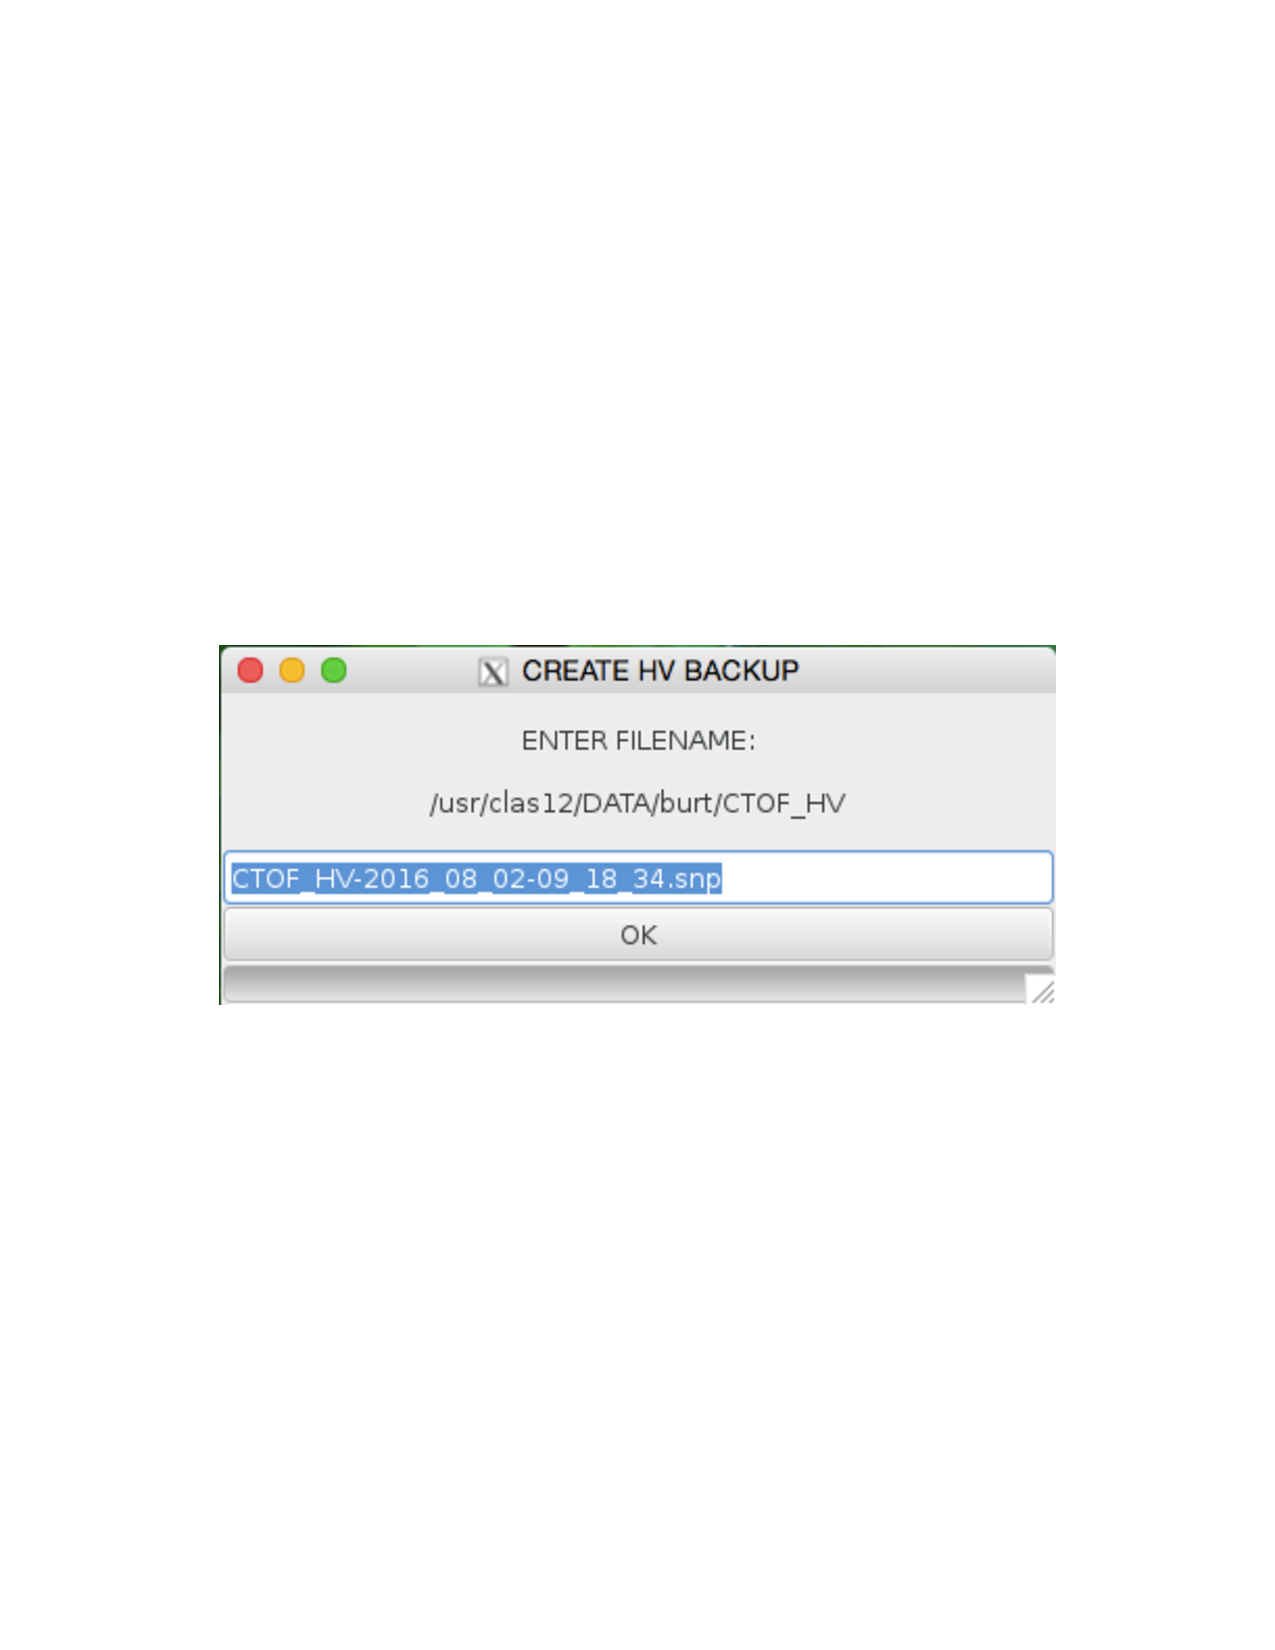
\includegraphics[width=0.80\textwidth,natwidth=610,natheight=642]
{ctof-backup.pdf}}}
\end{picture} 
\caption{Window that comes up after selecting ``Save Settings'' in 
Fig.~\ref{ctof-screen3-5}(right).}
\label{backup}
\end{figure}
%%%%%%%%%%%%%%%%%%%%%%%%%%%%%%%%%%%%%%%%%%%%%%%%%%%%%%%%%%%%%%%%%%%%%%%%%%%%%%%%%%%

\subsubsection{HV Save and Restore}
\label{save-restore}

The CTOF HV interface allows all system channel settings to be saved into a file 
or loaded from an archived file by clicking either on ``Save Settings'' or 
``Restore Settings'' on the CTOF Menu screen (see Fig.~\ref{ctof-screen3-5}(right)). 
The files created are referred to as ``BURT'' backup files, where BURT is an acronym 
for ``Backup and Restore Tool''. BURT is a utility for saving EPICS variables into 
an ASCII file readable by the EPICS Slow Controls system. The save files are stored 
on the DAQ machines in the Hall~B Counting House at: 
{\it /usr/clas12/DATA/burt/CTOF\_HV}.

Clicking on ``Save Settings'' brings up a window ``CREATE HV BACKUP'' as shown 
in Fig.~\ref{backup} showing the save file path and the pre-selected file name 
that contains the system name along with the date and time. If the ``Restore 
Settings'' option is chosen, the window shown in Fig.~\ref{restore} comes up 
showing the saved CTOF HV restore files available from which to select. Selecting 
a file and clicking on ``OK'' at the bottom of the window loads all channel 
parameters for the full HV system. Note that a new backup file should be created 
whenever any HV settings have changed, including HV values, channel parameter 
settings, or channel on/off settings.

%%%%%%%%%%%%%%%%%%%%%%%%%%%%%%%%%%%%%%%%%%%%%%%%%%%%%%%%%%%%%%%%%%%%%%%%%%%%%%%%%%%
\begin{figure}[htbp]
\vspace{3.7cm}
\begin{picture}(30,50) 
\put(50,220)
{\hbox{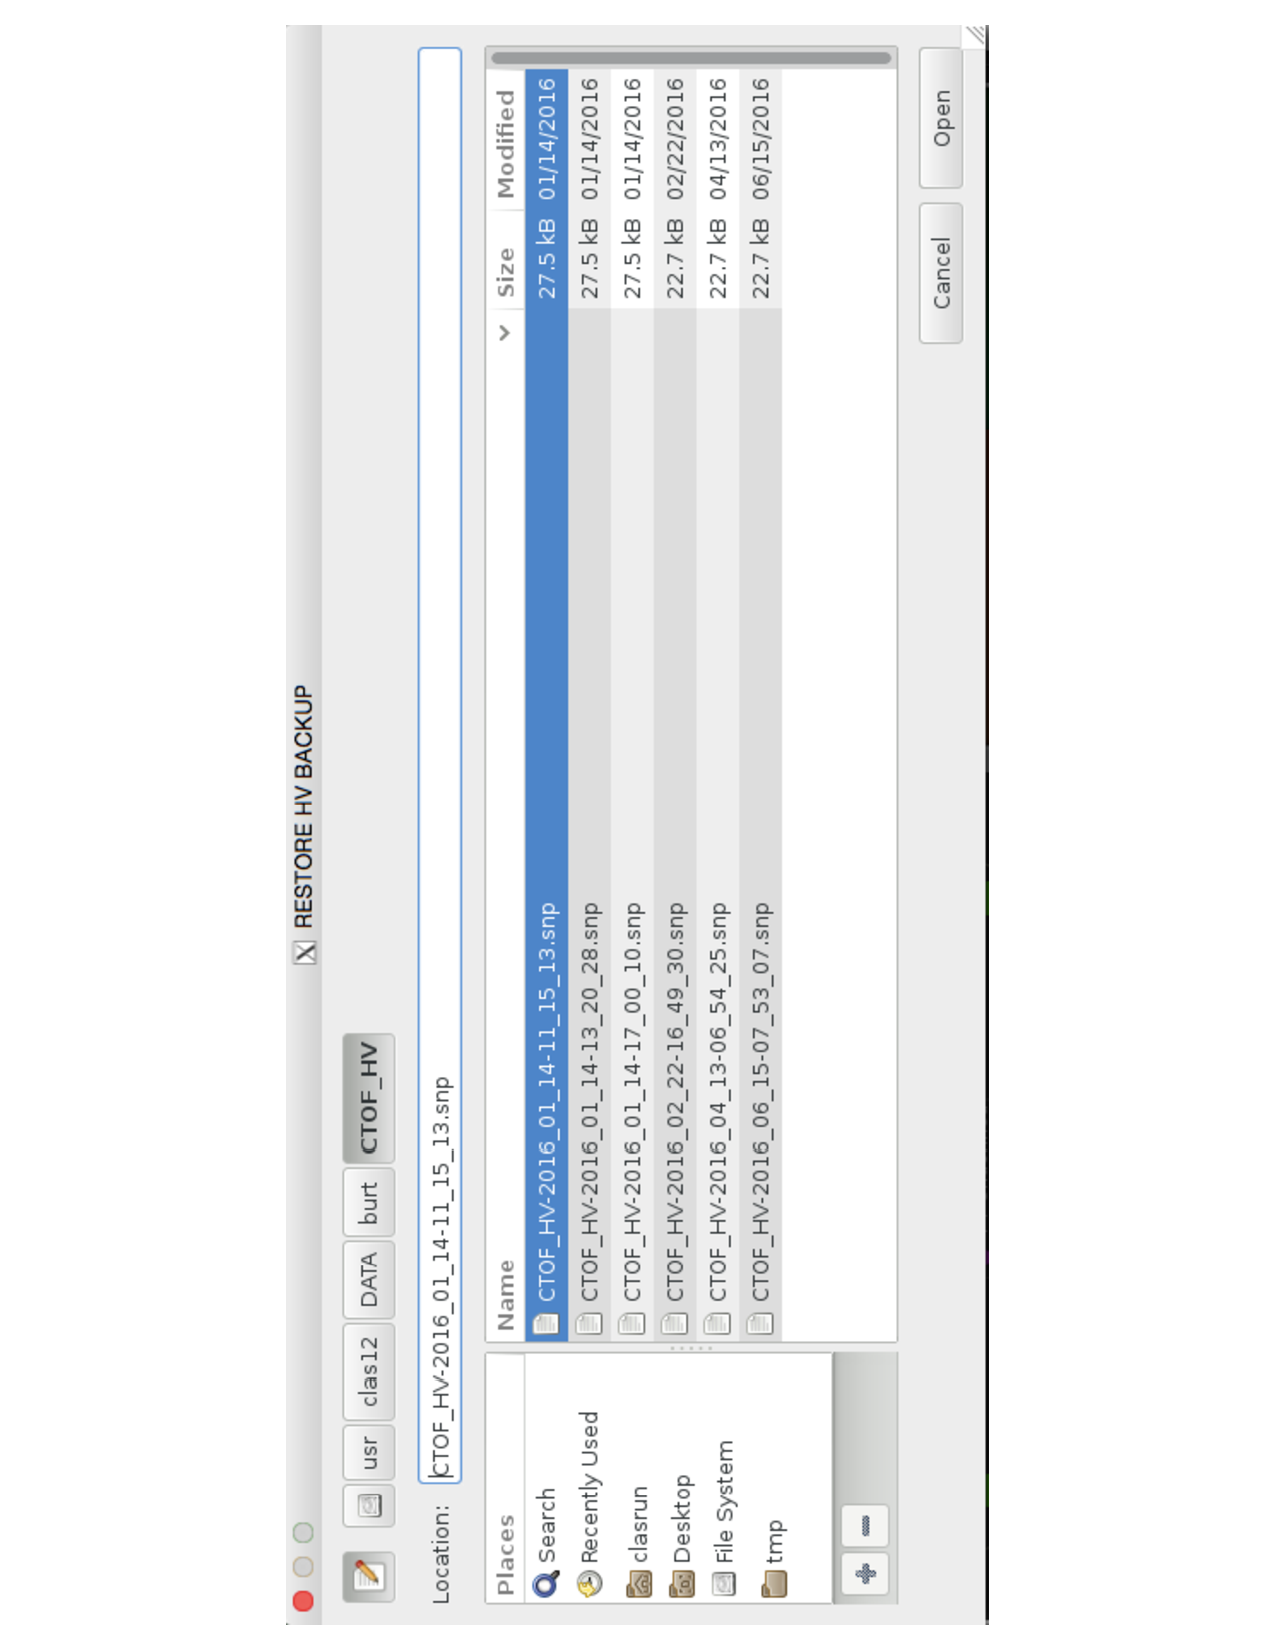
\includegraphics[width=0.60\textwidth,natwidth=610,natheight=642,angle=-90]
{ctof-restore.pdf}}}
\end{picture} 
\caption{Window that comes up after selecting ``Restore Settings'' in 
Fig.~\ref{ctof-screen3-5}(right).}
\label{restore}
\end{figure}
%%%%%%%%%%%%%%%%%%%%%%%%%%%%%%%%%%%%%%%%%%%%%%%%%%%%%%%%%%%%%%%%%%%%%%%%%%%%%%%%%%%

\subsection{Cabling Details}

\subsubsection{Signal Cable Connections}
\label{signal-conn}

The signal cables for each PMT run from the voltage divider to one of two UVa 
80-20 signal splitters. A schematic diagram of the splitter connections is shown 
in Fig.~\ref{ctof-splitter}. The 80\% signals run from the splitters to the 
discriminators. Fig.~\ref{ctof-disc-map} shows the signal mapping to the 
discriminators. The discriminator outputs are then connected to the TDCs. The 
20\% signals run from the splitters to the FADC inputs. The splitter outputs to 
the FADCs are through 34-pin connectors for each of the four groups (see 
Fig.~\ref{ctof-splitter}). The splitter outputs to the discriminators are through 
the lemo connectors.

The CTOF channel connections to the VME readout electronics are mapped in such a 
way that neighboring PMTs are not connected to neighboring electronics inputs. 
This scheme was devised to reduce any electronics noise coupling (i.e. cross-talk). 
The VME electronics channel mapping is shown in Figs.~\ref{ctof-vme1-map} and 
\ref{ctof-vme2-map} for the TDCs and FADCs, respectively. Fig.~\ref{cable-types} 
gives schematics for the cable and connector types for each segment of the 
connections from the voltage divider to the readout electronics for the CTOF 
counters.

%%%%%%%%%%%%%%%%%%%%%%%%%%%%%%%%%%%%%%%%%%%%%%%%%%%%%%%%%%%%%%%%%%%%%%%%%%%%%%%%%%%
\begin{figure}[htbp]
\vspace{17.0cm}
\begin{picture}(30,50) 
\put(15,0)
{\hbox{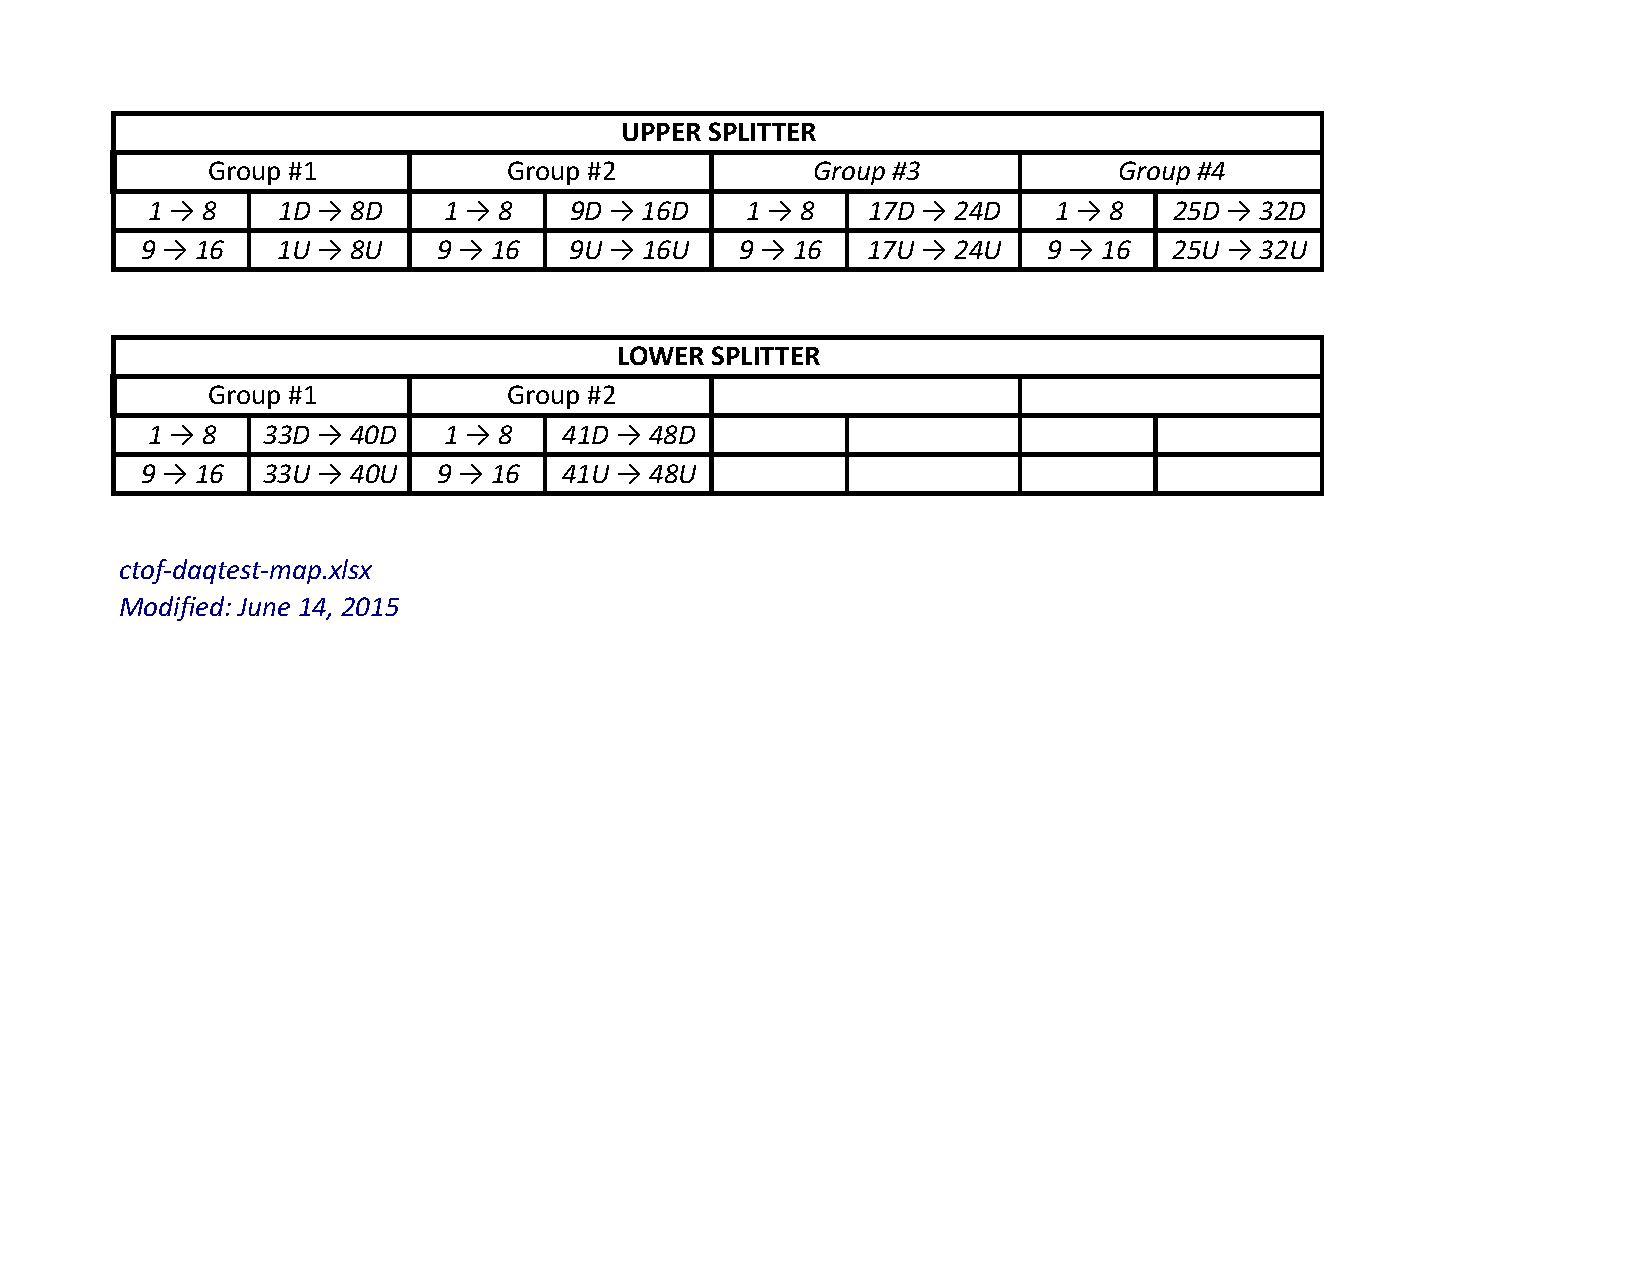
\includegraphics[width=0.85\textwidth,natwidth=610,natheight=642]
{ctof-splitter.pdf}}}
\end{picture} 
\caption{Layout of the connections to the two CTOF signal splitters.}
\label{ctof-splitter}
\end{figure}
%%%%%%%%%%%%%%%%%%%%%%%%%%%%%%%%%%%%%%%%%%%%%%%%%%%%%%%%%%%%%%%%%%%%%%%%%%%%%%%%%%%

%%%%%%%%%%%%%%%%%%%%%%%%%%%%%%%%%%%%%%%%%%%%%%%%%%%%%%%%%%%%%%%%%%%%%%%%%%%%%%%%%%%
\begin{figure}[htbp]
\vspace{12.0cm}
\begin{picture}(30,50) 
\put(45,0)
{\hbox{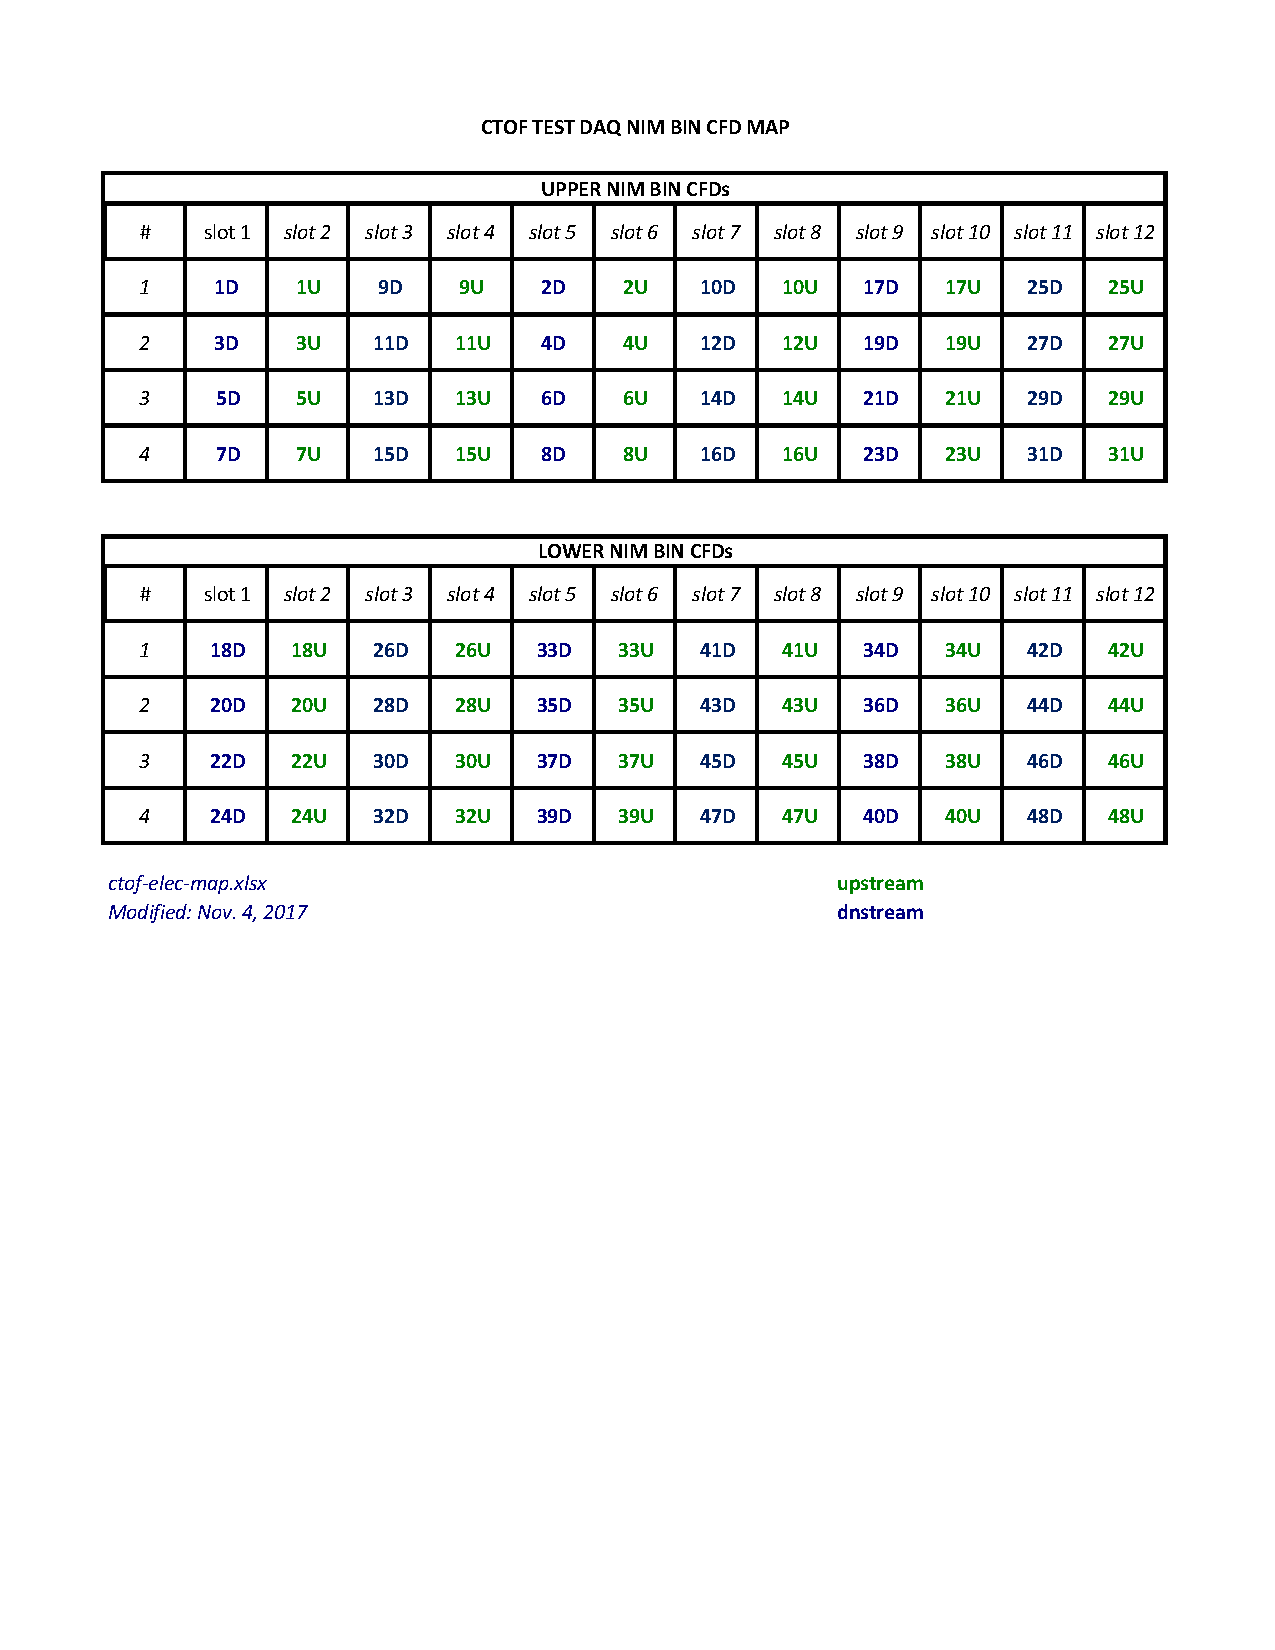
\includegraphics[width=0.75\textwidth,natwidth=610,natheight=642]{ctof-nim.pdf}}}
\end{picture} 
\caption{Mapping of the CTOF counters to the CFDs.}
\label{ctof-disc-map}
\end{figure}
%%%%%%%%%%%%%%%%%%%%%%%%%%%%%%%%%%%%%%%%%%%%%%%%%%%%%%%%%%%%%%%%%%%%%%%%%%%%%%%%%%%

%%%%%%%%%%%%%%%%%%%%%%%%%%%%%%%%%%%%%%%%%%%%%%%%%%%%%%%%%%%%%%%%%%%%%%%%%%%%%%%%%%%
\begin{figure}[htbp]
\vspace{17.0cm}
\begin{picture}(30,50) 
\put(15,0)
{\hbox{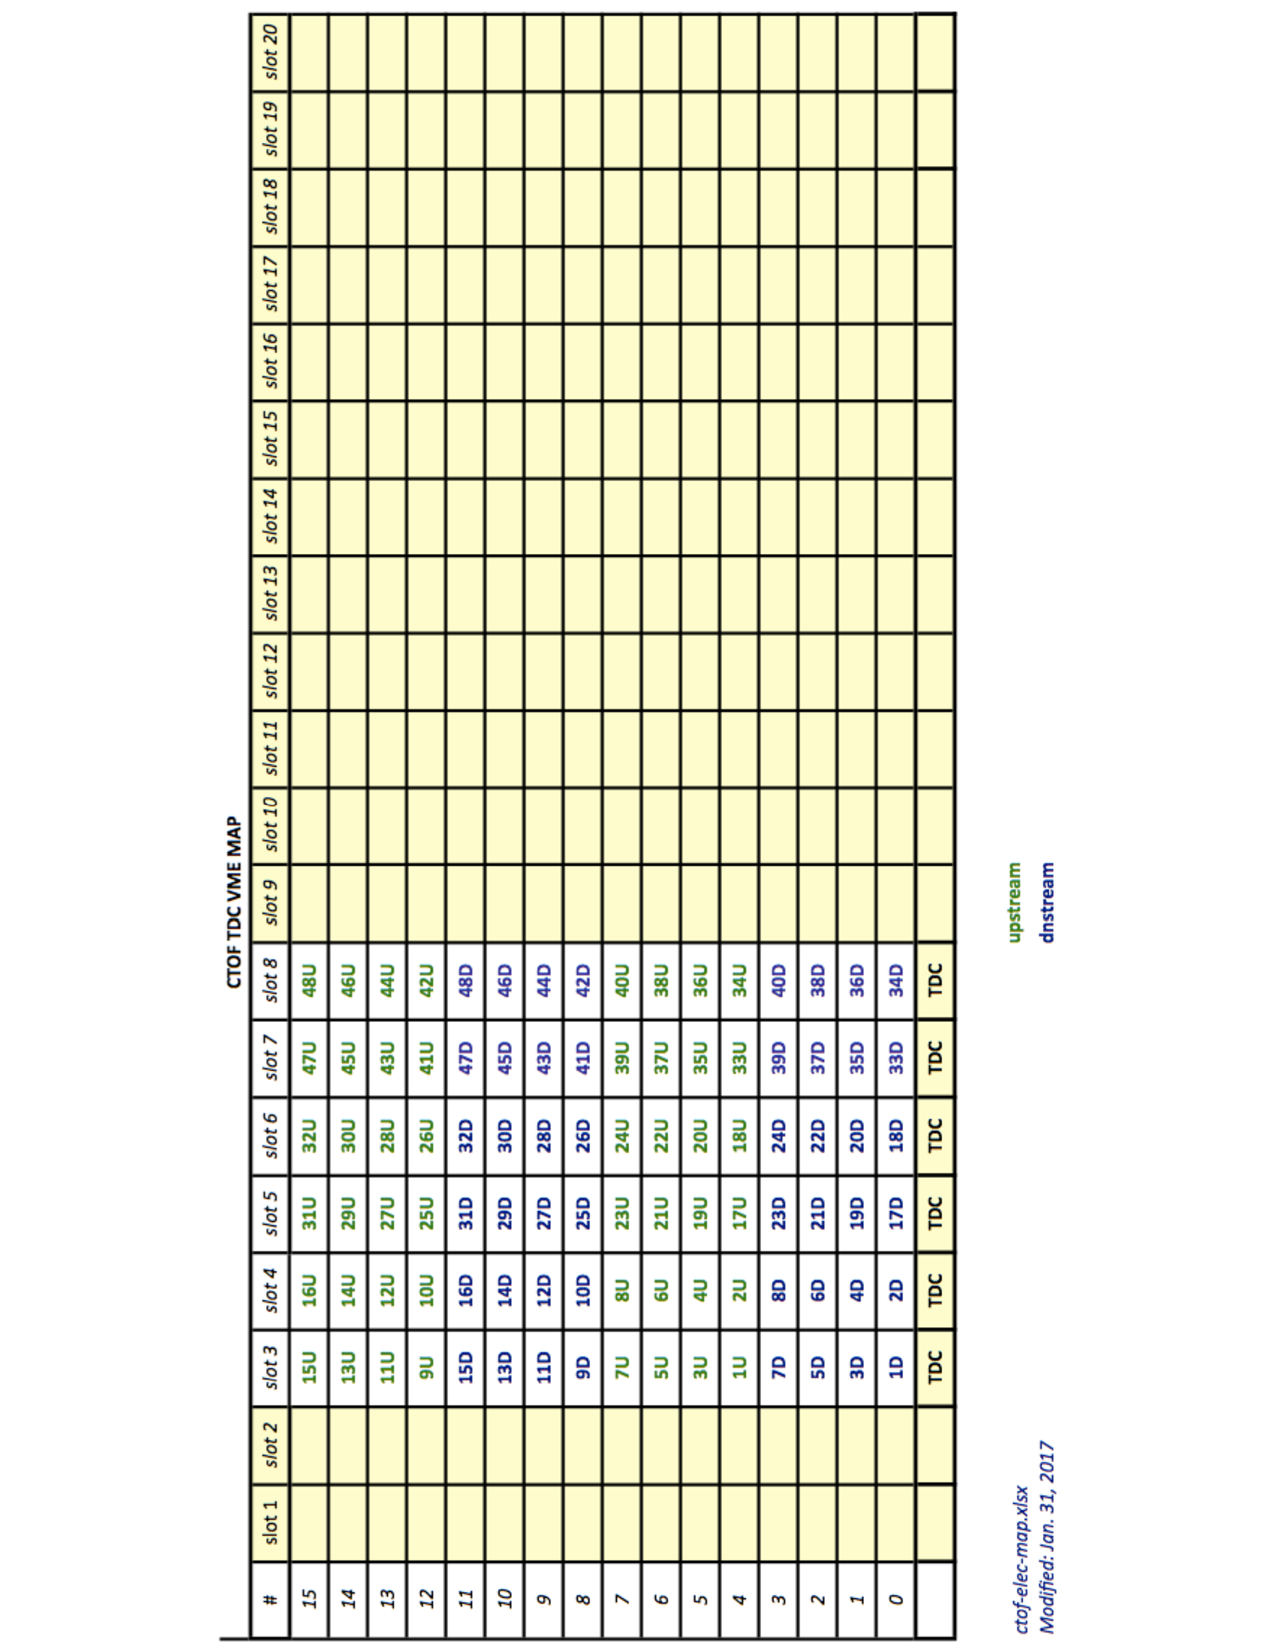
\includegraphics[width=0.95\textwidth,natwidth=610,natheight=642]{ctof-vme1.pdf}}}
\end{picture} 
\caption{CTOF VME map for the TDCs.}
\label{ctof-vme1-map}
\end{figure}
%%%%%%%%%%%%%%%%%%%%%%%%%%%%%%%%%%%%%%%%%%%%%%%%%%%%%%%%%%%%%%%%%%%%%%%%%%%%%%%%%%%

%%%%%%%%%%%%%%%%%%%%%%%%%%%%%%%%%%%%%%%%%%%%%%%%%%%%%%%%%%%%%%%%%%%%%%%%%%%%%%%%%%%
\begin{figure}[htbp]
\vspace{17.0cm}
\begin{picture}(30,50) 
\put(15,0)
{\hbox{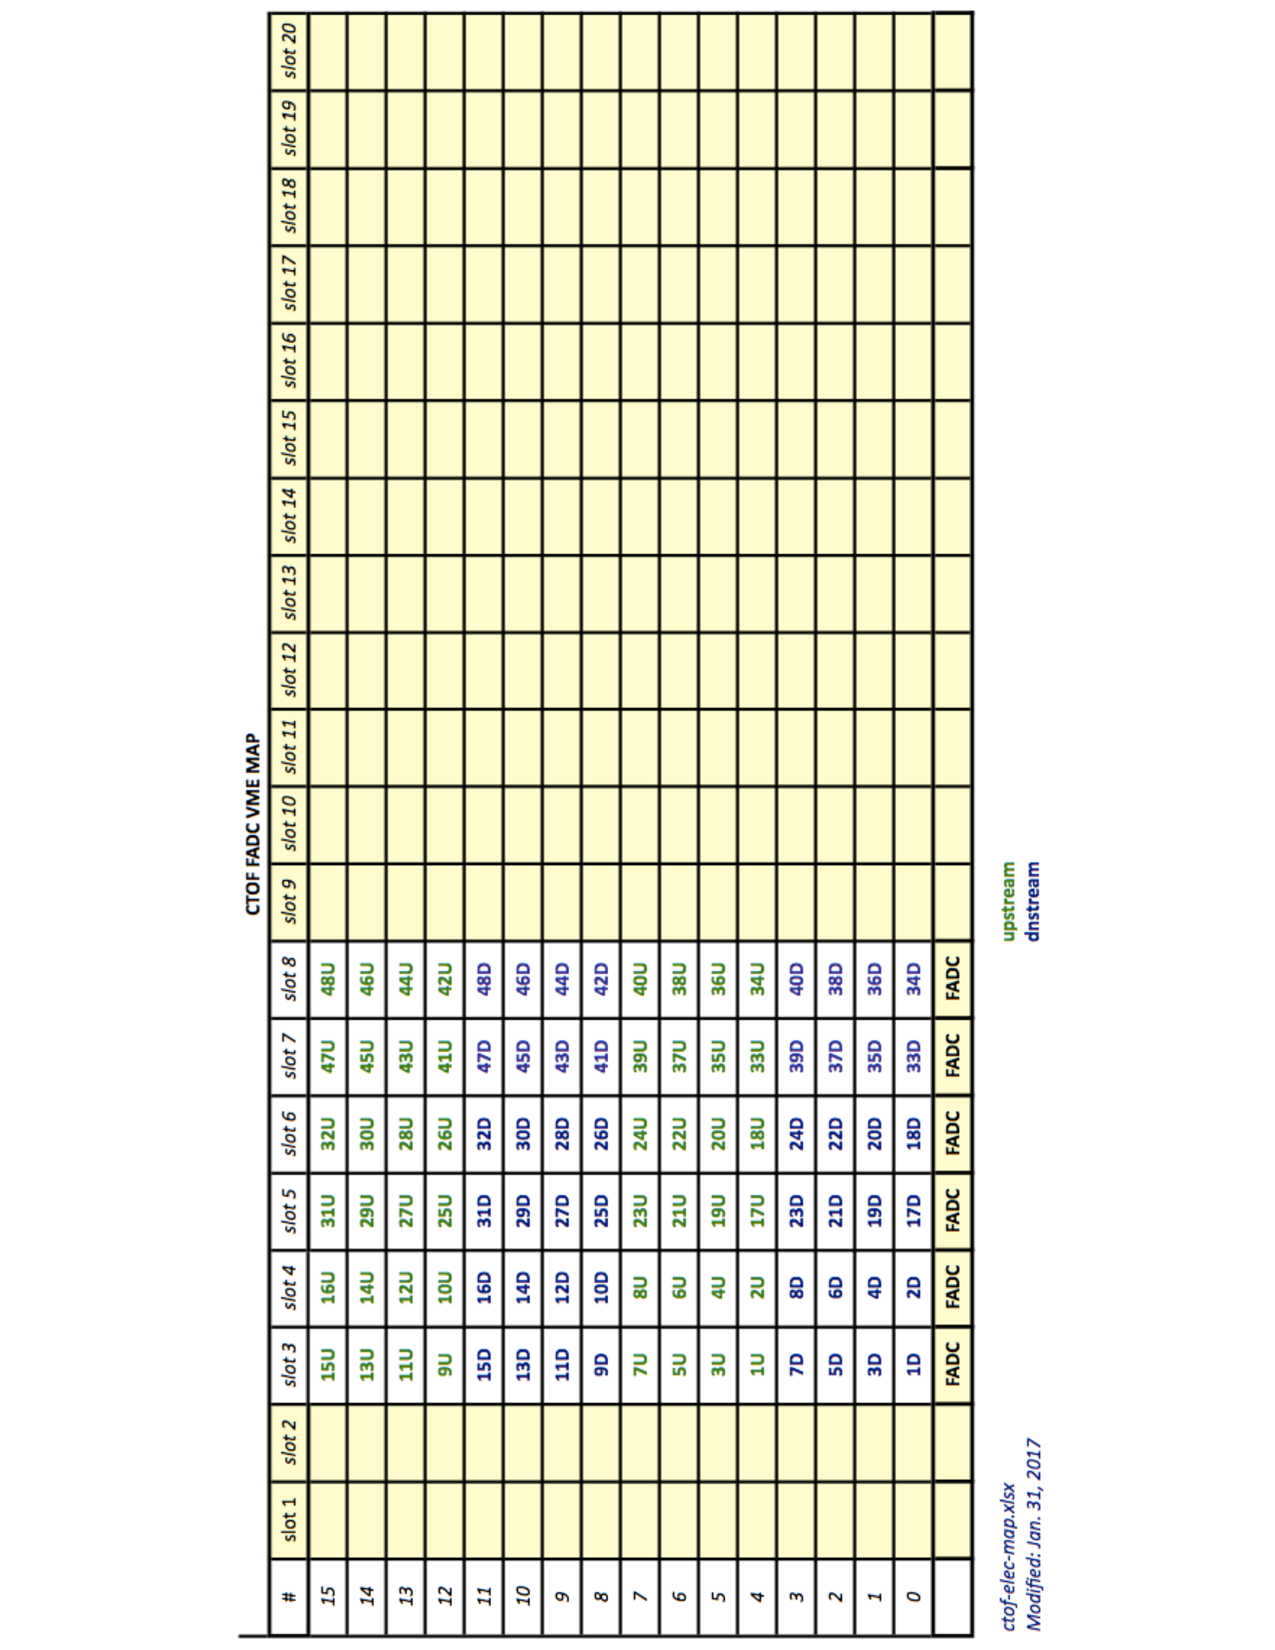
\includegraphics[width=0.95\textwidth,natwidth=610,natheight=642]{ctof-vme2.pdf}}}
\end{picture} 
\caption{CTOF VME map for the FADCs.}
\label{ctof-vme2-map}
\end{figure}
%%%%%%%%%%%%%%%%%%%%%%%%%%%%%%%%%%%%%%%%%%%%%%%%%%%%%%%%%%%%%%%%%%%%%%%%%%%%%%%%%%%

%%%%%%%%%%%%%%%%%%%%%%%%%%%%%%%%%%%%%%%%%%%%%%%%%%%%%%%%%%%%%%%%%%%%%%%%%%%%%%%%%%%
\begin{figure}[htbp]
\vspace{7.5cm}
\begin{picture}(30,50) 
\put(0,350)
{\hbox{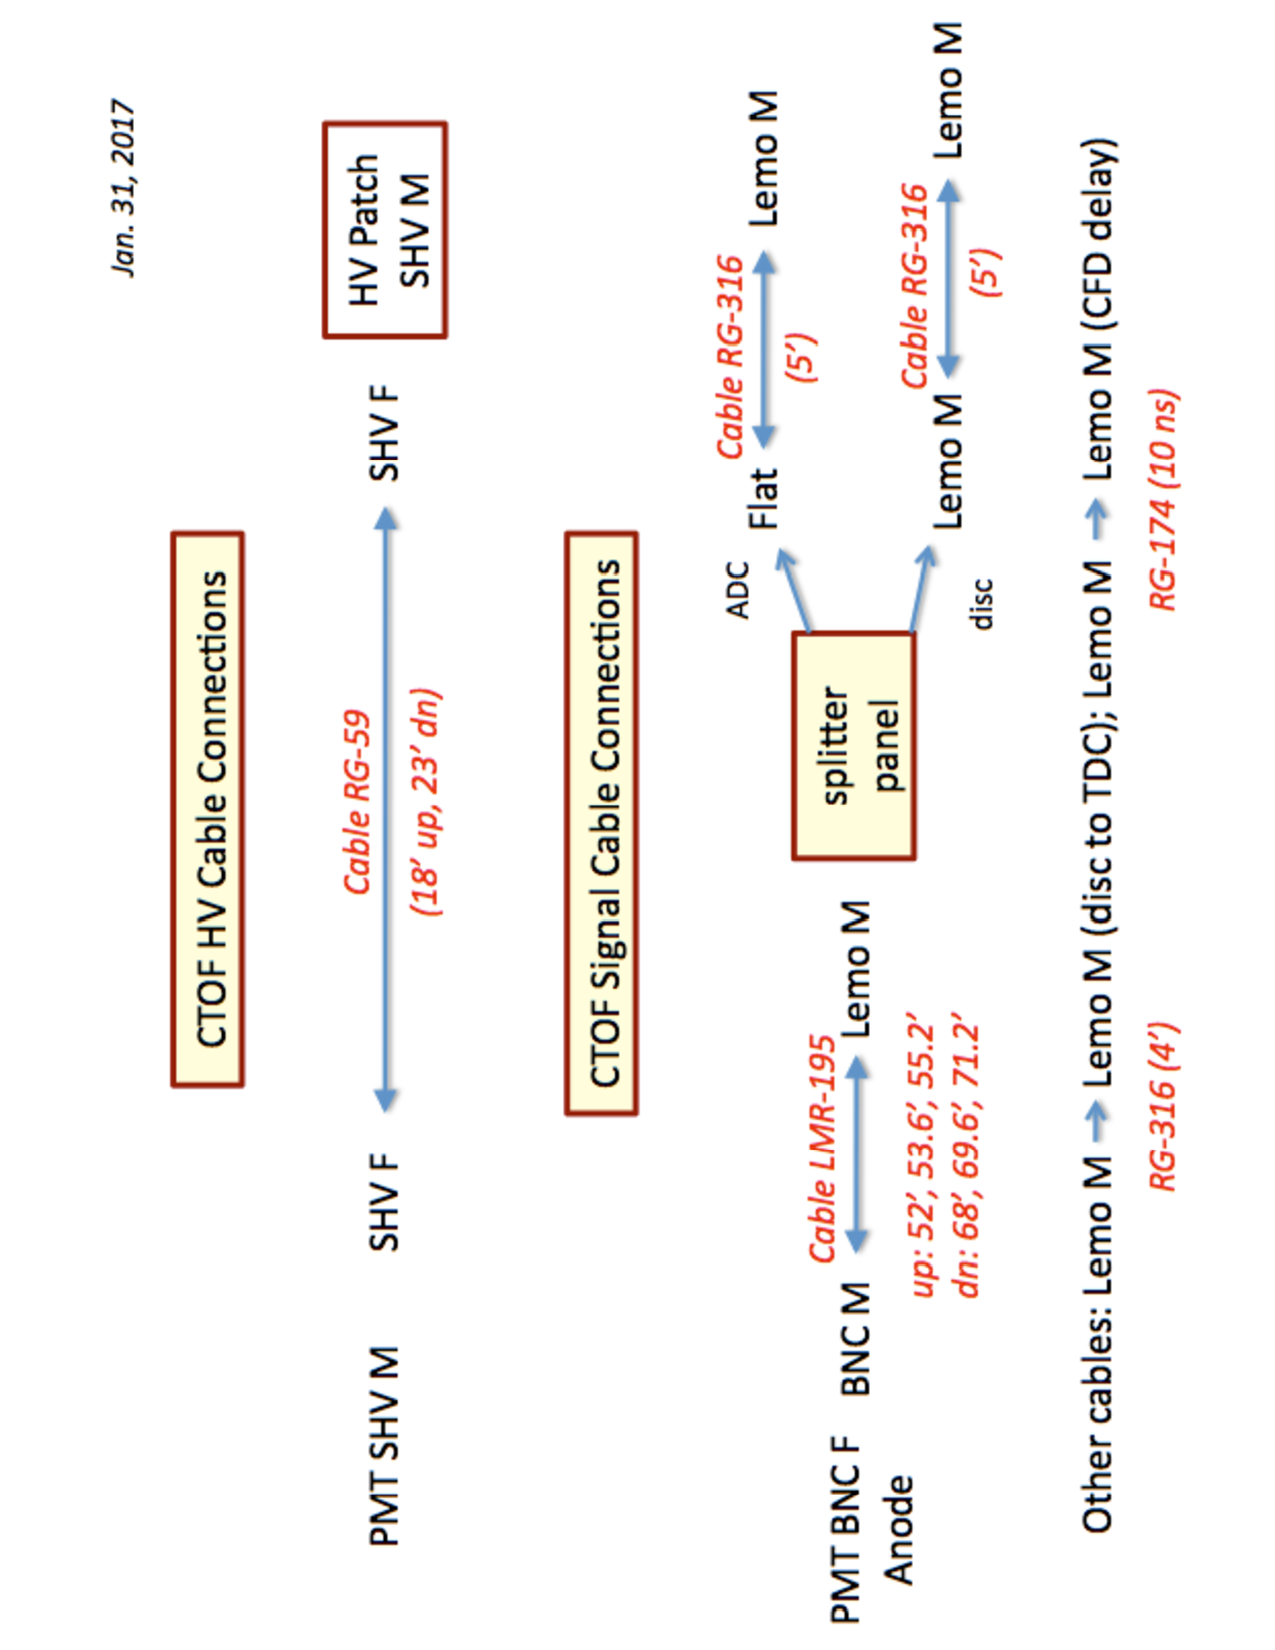
\includegraphics[width=0.75\textwidth,natwidth=610,natheight=642,angle=-90]
{cable-types.pdf}}}
\end{picture} 
\caption{CTOF HV and signal cable connections.}
\label{cable-types}
\end{figure}
%%%%%%%%%%%%%%%%%%%%%%%%%%%%%%%%%%%%%%%%%%%%%%%%%%%%%%%%%%%%%%%%%%%%%%%%%%%%%%%%%%%

\clearpage

\subsubsection{HV Cable Layout}
\label{hv-layout}

The high voltage cables for each PMT run from the voltage divider to one of two 
HV distribution boxes located on the solenoid cart. Fig.~\ref{ctof-hv-map} shows 
the layout of the two HV distribution boxes for the upstream and downstream PMT 
HV connections. The output of each HV distribution box is a pair of 55-ft-long 
multi-conductor cables, each containing 24-channels, with a Radiall connector to 
mate with the HV A1535N board input connector. See Fig.~\ref{cable-types} for 
schematics of the cable and connector types for each segment of the HV connections 
from the voltage divider to the HV power supplies for the counters in CTOF. The 
HV power supply channel assignments for each sector are nominally given as shown 
in Fig.~\ref{ctof-hvmap}.

%%%%%%%%%%%%%%%%%%%%%%%%%%%%%%%%%%%%%%%%%%%%%%%%%%%%%%%%%%%%%%%%%%%%%%%%%%%%%%%%%%%
\begin{figure}[htbp]
\vspace{5.7cm}
\begin{picture}(30,50) 
\put(45,-65)
{\hbox{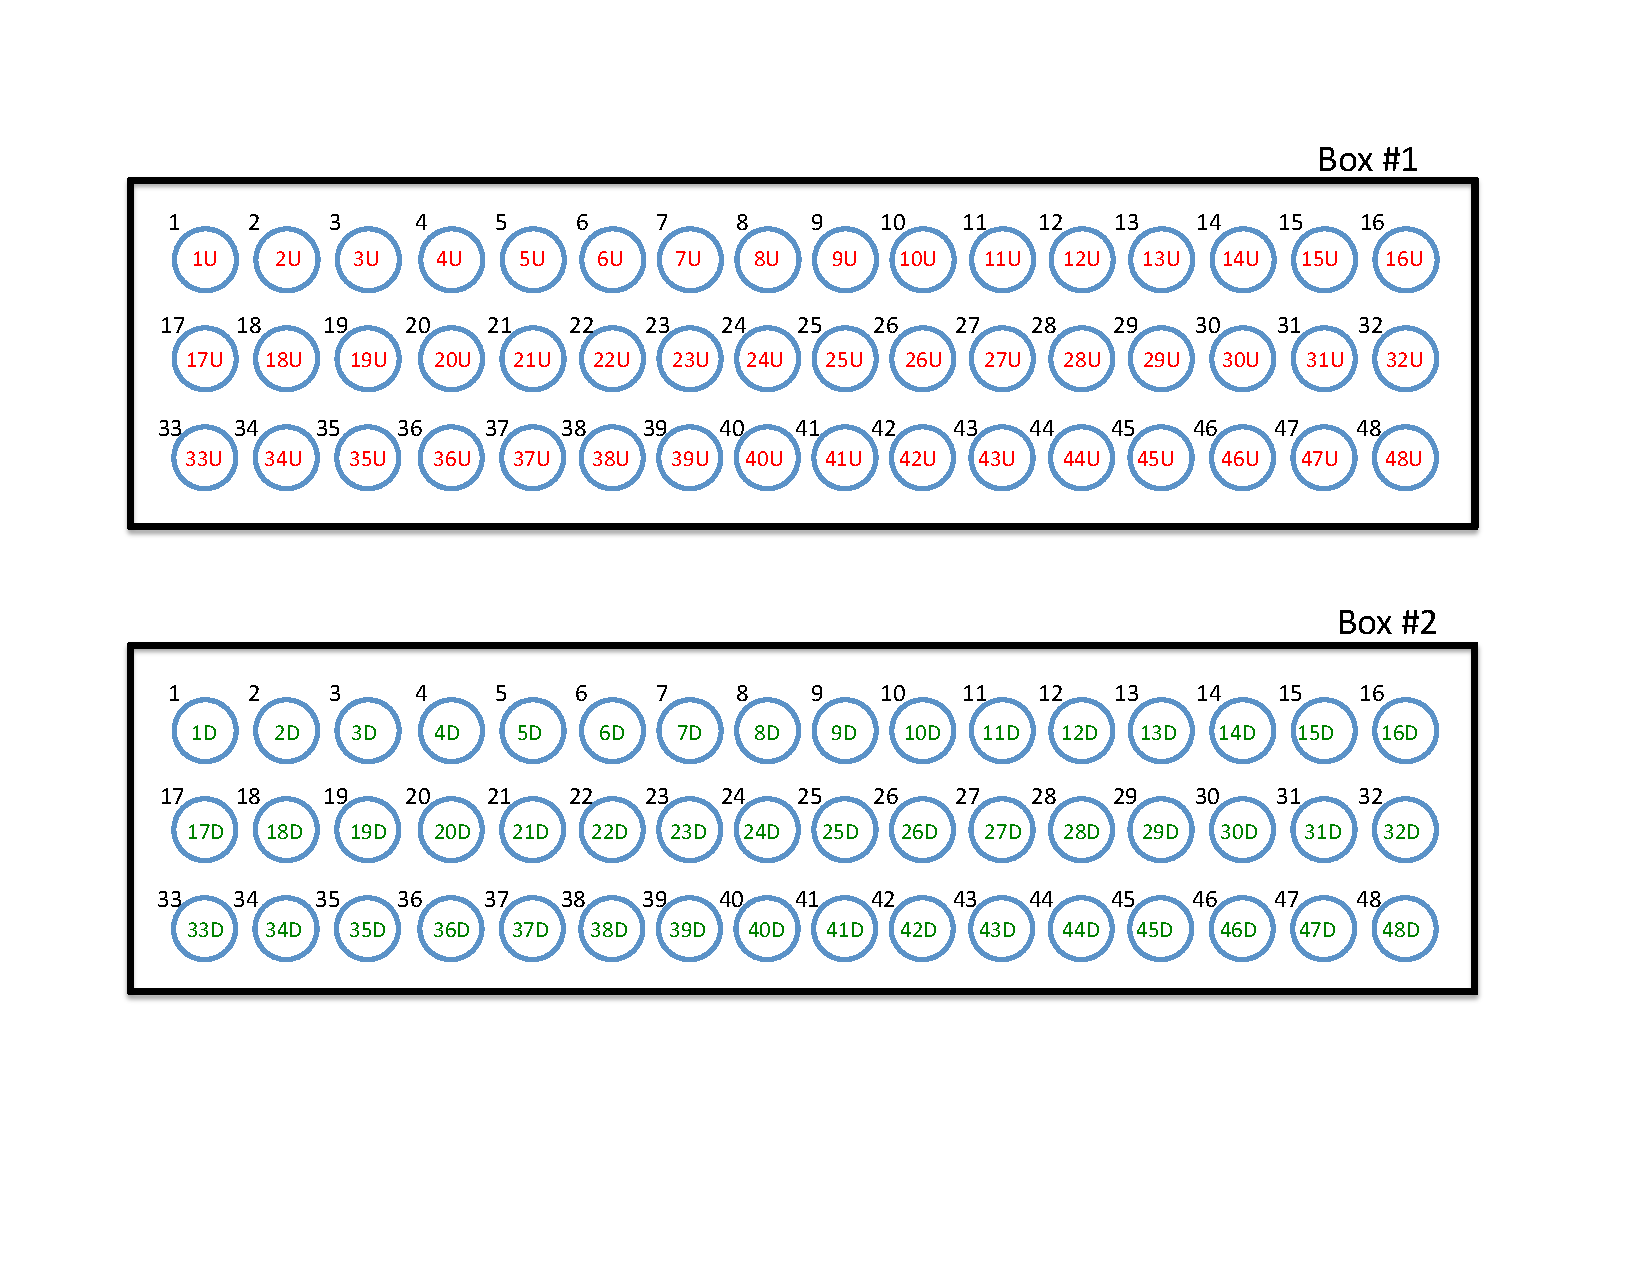
\includegraphics[width=0.65\textwidth,natwidth=610,natheight=642]
{ctof-hv-map.pdf}}}
\end{picture} 
\caption{Mapping of the HV channel connections to the HV distribution boxes for 
the upstream and downstream PMTs.}
\label{ctof-hv-map}
\end{figure}
%%%%%%%%%%%%%%%%%%%%%%%%%%%%%%%%%%%%%%%%%%%%%%%%%%%%%%%%%%%%%%%%%%%%%%%%%%%%%%%%%%%

%%%%%%%%%%%%%%%%%%%%%%%%%%%%%%%%%%%%%%%%%%%%%%%%%%%%%%%%%%%%%%%%%%%%%%%%%%%%%%%%%%%
\begin{figure}[htbp]
\vspace{3.0cm}
\begin{picture}(30,50) 
\put(30,-370)
{\hbox{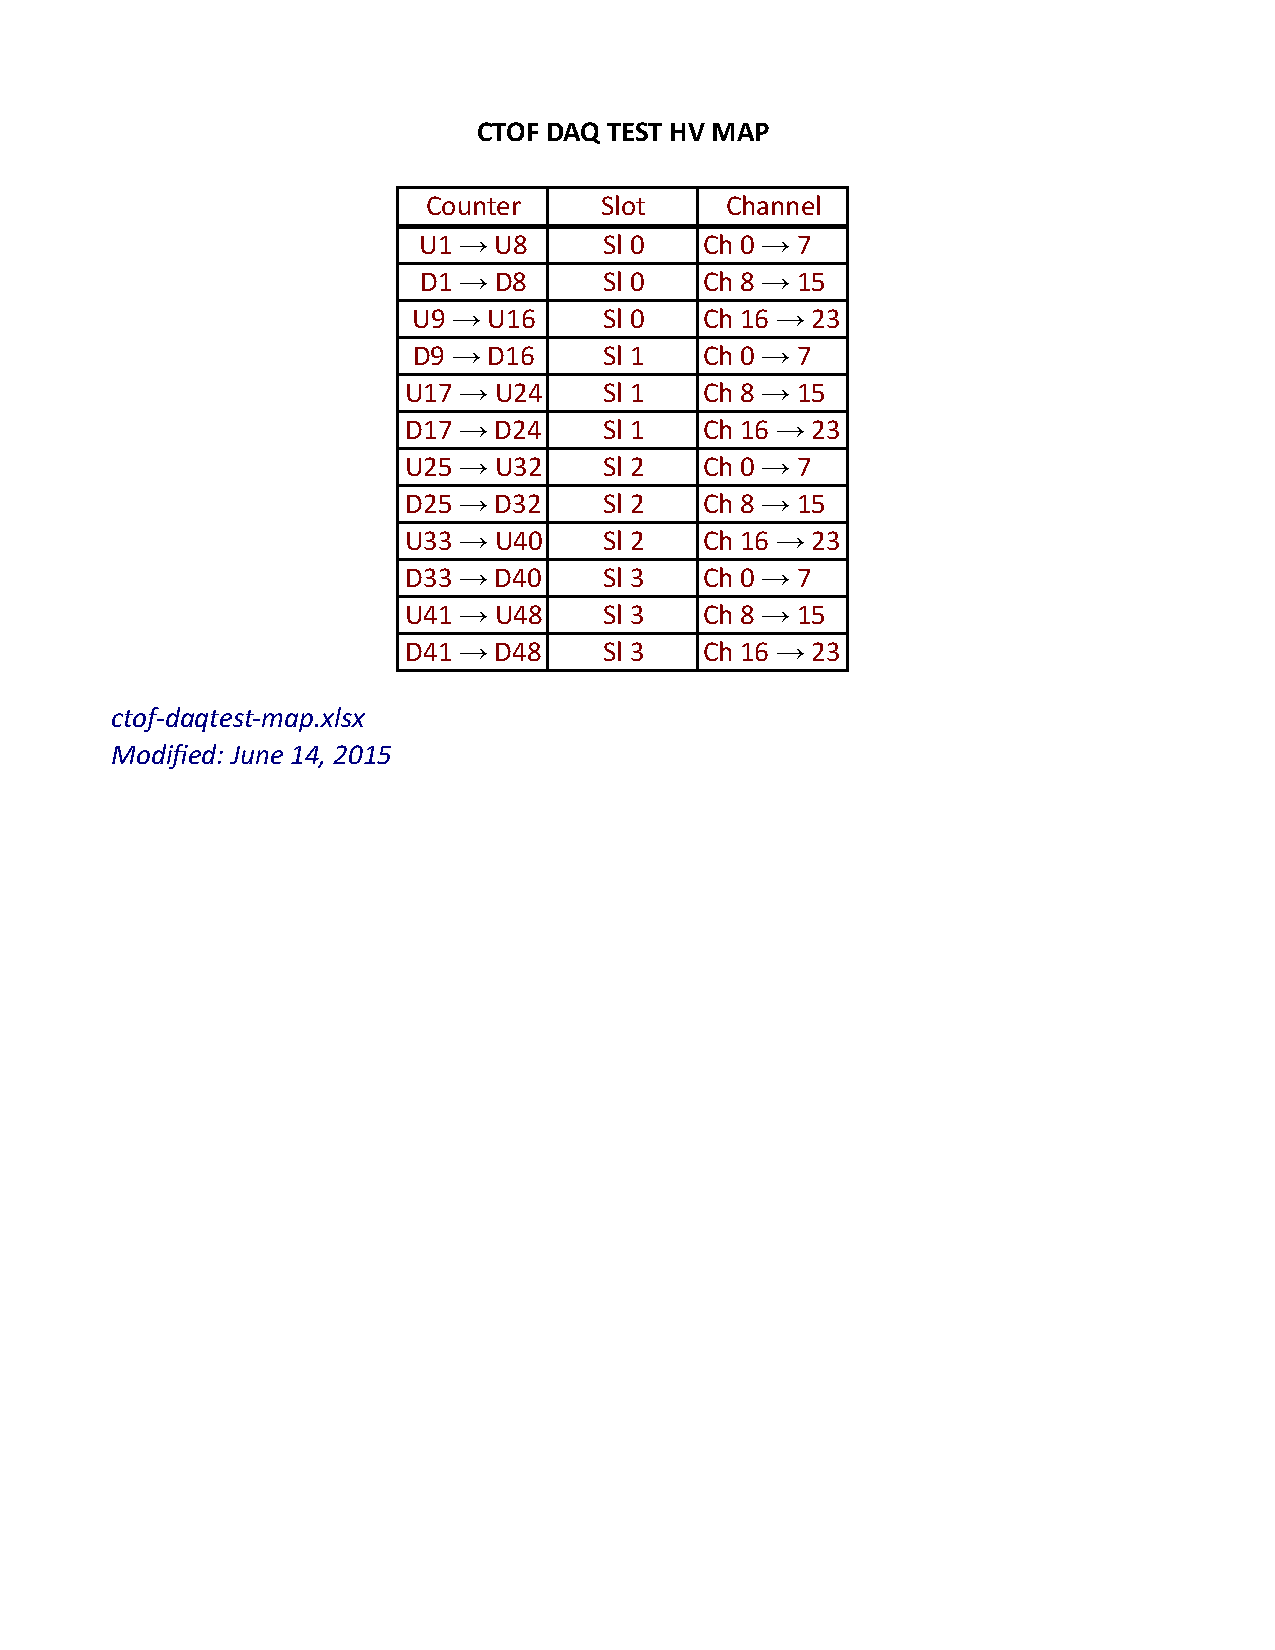
\includegraphics[width=0.90\textwidth,natwidth=610,natheight=642]{ctof-hv.pdf}}}
\end{picture} 
\caption{HV mainframe CTOF channel assignments.}
\label{ctof-hvmap}
\end{figure}
%%%%%%%%%%%%%%%%%%%%%%%%%%%%%%%%%%%%%%%%%%%%%%%%%%%%%%%%%%%%%%%%%%%%%%%%%%%%%%%%%%%

\subsubsection{Altering Cable Maps}

The nominal procedure if there is a problem with a VME electronics board is to 
replace the board with a spare unit. However, for testing purposes, it might be 
necessary to change a signal input at the FADC or TDC to an unused channel. This 
work must always be done in coordination with the DAQ system expert in order to 
update the channel map used as input to the translation table. This operation is 
not something that is normally done and should not be attempted by shift workers 
or CTOF experts as it could lead to problems decoding the data.

Problems with channels within the HV system are more common issues as channels on 
the HV distribution box or on a A1535N card are reasonably common. The standard 
procedure when there is a problem with a CAEN HV board is to swap out the board 
(see Section~\ref{board-swap}). If there is a problem on the HV distribution box 
for either the upstream or downstream PMTs, the box would have to be swapped out 
with a spare unit. The first step before disconnecting any system HV cables is to 
be sure that the associated HV channels are turned off. The SHV cables can then be 
disconnected. If there is a need to update the HV channels map, contact the Slow 
Controls expert.

\subsection{Detector Repairs and Servicing}

Repairs and servicing on the CTOF detectors themselves are highly involved operations. 
If there were a problem with the scintillation bars or a glue joint, it might be the 
case that the counters would have to be removed from the solenoid. However, PMTs that 
go bad can be replaced relatively easily. In addition, voltage dividers can also 
sometimes go bad due to failed components. All work on the CTOF detectors must be 
coordinated with the CTOF Group Leader and the Hall~B Work Coordinator during an 
access period with the solenoid turned off.

\clearpage

\vfil
\eject

\section{Documentation}

All current documentation for the CTOF system is located on the official CTOF web 
page~\cite{ctof-web}. A number of basic subsystem documents can be found there 
including:

\begin{itemize}
\item CTOF System Operations Manual (this document)
 \begin{itemize}
   \item The source files for the CTOF System Operations Manual are located on the
         github repository at: {\it JeffersonLab/clas12-manuals}
 \end{itemize}
\item CTOF Geometry Document
\item CTOF Calibration Constants
\item CTOF Monte Carlo Simulation Details
\item CTOF Reconstruction Document
\item CTOF Counter Wrapping Procedures
\item CTOF Magnetic Shield Attachment Procedures
\item CTOF Calibration Algorithms
\item CTOF Calibration Tutorial
\item Assorted photographs of the detector hardware
\end{itemize}

If you have any questions related to any of the CTOF system documentation, please 
contact the CTOF Group Leader.

\section{CTOF Authorized Personnel}
\label{personnel}

Beyond turning on/off the CTOF system HV and monitoring the system scalers, all other 
operations and repairs are only to be carried out by the list of authorized personnel 
shown in Table~\ref{expert-list}. The list of authorized personnel for CTOF can only 
be modified by the CTOF Group Leader.

%%%%%%%%%%%%%%%%%%%%%%%%%%%%%%%%%%%%%%%%%%%%%%%%%%%%%%%%%%%%%%%%%%%%%%%%%%%%%%%%%%%
\begin{table}[htbp]
\begin{center}
\begin{tabular} {|c|c|c|c|} \hline
Name             & Telephone      & email              & Area             \\ \hline \hline
Daniel S. Carman & (757)-269-5586 & carman@jlab.org    & CTOF Group Leader\\
                 &                &                    & Hardware, Software \\ \hline
Cole Smith       & (757)-269-5307 & lcsmith@jlab.org   & Hardware, {\it CTOFMON} \\ \hline
Sergey Boyarinov & (757)-269-5795 & boyarinov@jlab.org & DAQ              \\ \hline
Nathan Baltzell  & (757)-269-5902 & baltzell@jlab.org  & Slow Controls    \\ \hline
\end{tabular}
\caption{CTOF detector authorized personnel.}
\label{expert-list}
\end{center}
\end{table}
%%%%%%%%%%%%%%%%%%%%%%%%%%%%%%%%%%%%%%%%%%%%%%%%%%%%%%%%%%%%%%%%%%%%%%%%%%%%%%%%%%%

\clearpage

\vfil
\eject

\section{Appendix: Hall~B Instrumentation Database}

When electronics modules or HV modules are removed from Hall~B and replaced during 
servicing with new boards, the information regarding both the old board and the new 
board needs to be entered into the Hall~B Instrumentation Database. This database is 
accessed online at {\it http://clonwiki0.jlab.org} by clicking on the ``Hall~B Inventory'' 
link. This brings up the access screen shown in Fig.~\ref{inventory}. To enter 
information for the old component, search for it in the database using its property 
tag information. When the item shows up, click on the ``Action'' button for ``Modify 
this item''. Be sure to change the location of the item to ``Hall~B Underground/RadCon 
Table'' and change the status of the item to ``Action needed/Broken'', as well as to 
leave the item on the RadCon survey table in Hall~B. By entering this information, 
email will be sent to the property custodian to pick up the item for servicing. For 
the new component, be sure to also change the location as appropriate using the same 
approach.

%%%%%%%%%%%%%%%%%%%%%%%%%%%%%%%%%%%%%%%%%%%%%%%%%%%%%%%%%%%%%%%%%%%%%%%%%%%%%%%%%%%
\begin{figure}[htbp]
\vspace{7.2cm}
\begin{picture}(30,50) 
\put(5,305)
{\hbox{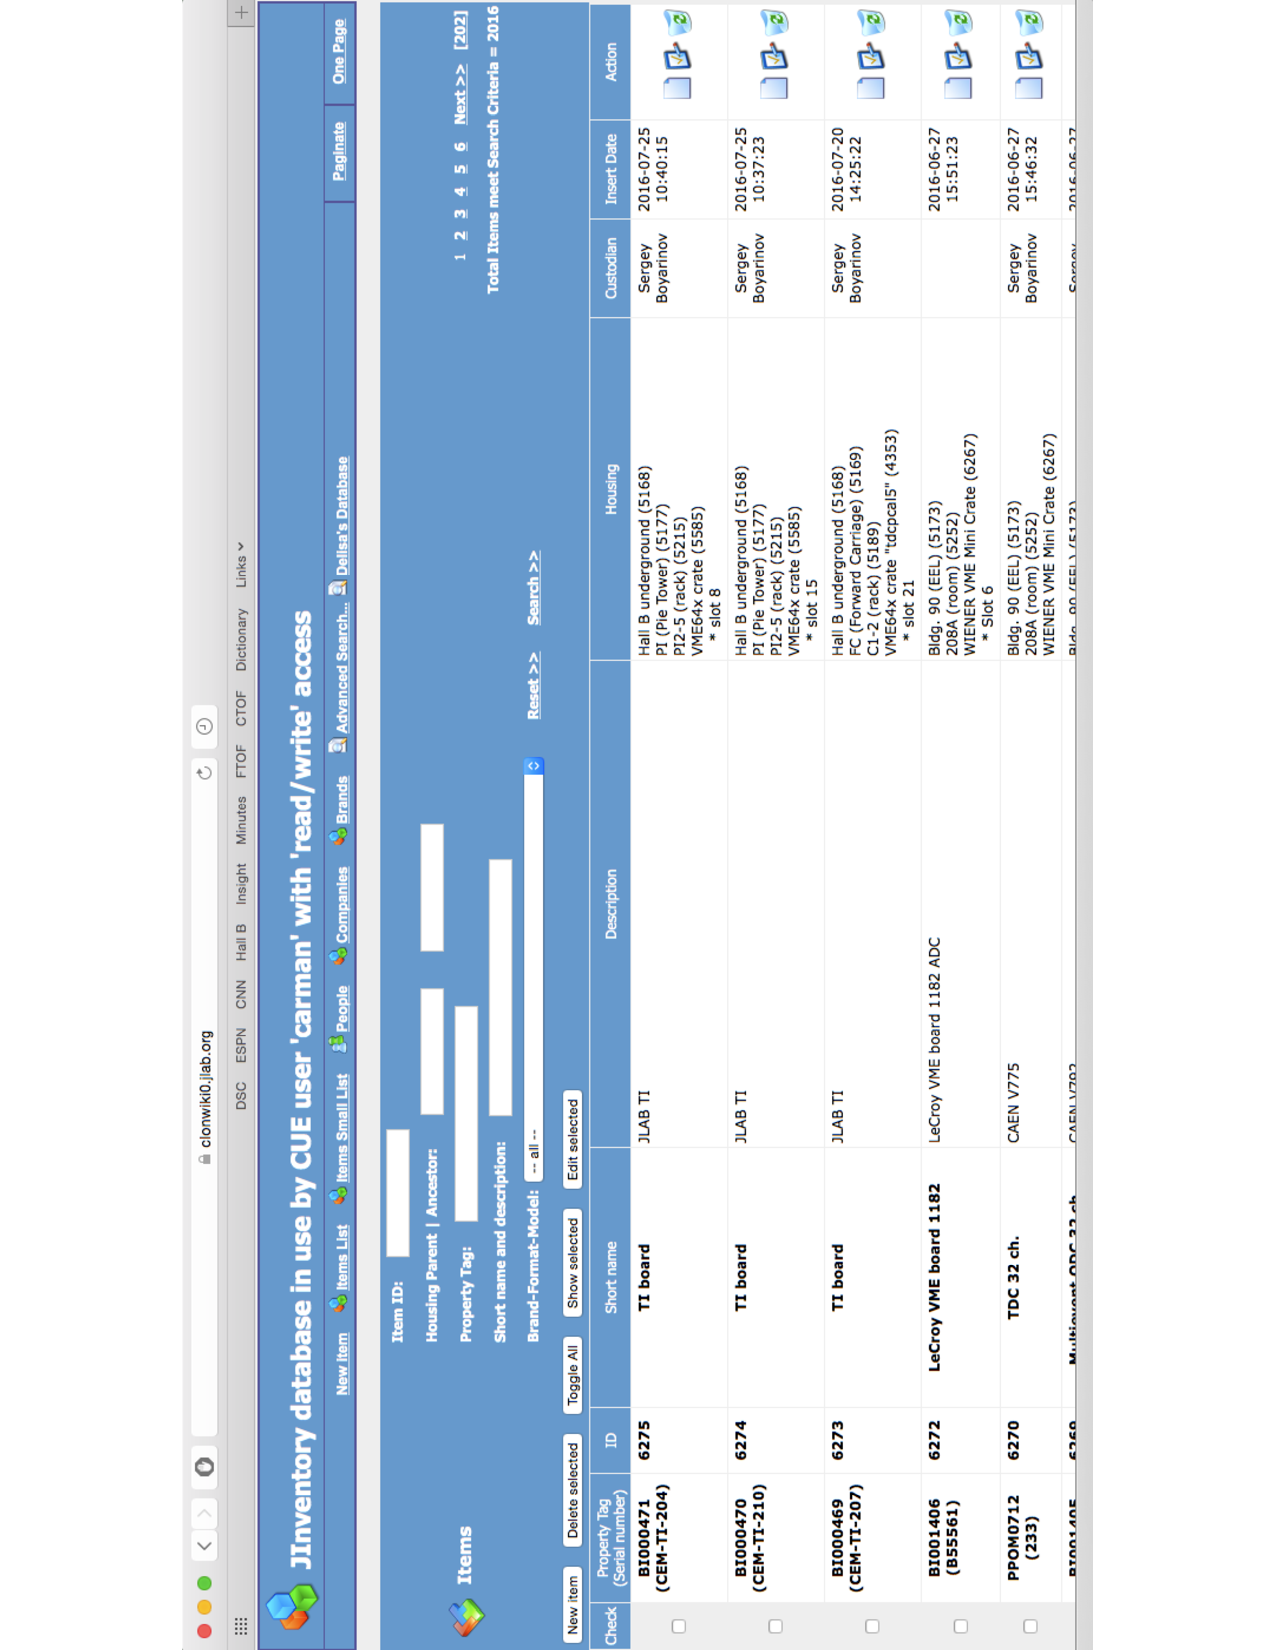
\includegraphics[width=0.75\textwidth,natwidth=610,natheight=642,angle=-90]
{inventory.pdf}}}
\end{picture} 
\caption{Hall~B equipment database web page.}
\label{inventory}
\end{figure}
%%%%%%%%%%%%%%%%%%%%%%%%%%%%%%%%%%%%%%%%%%%%%%%%%%%%%%%%%%%%%%%%%%%%%%%%%%%%%%%%%%%

\clearpage

\vfil
\eject

\begin{thebibliography}{99}

\bibitem{e-log}
Hall~B Electronic Logbook: https://logbooks.jlab.org/book/hblog

\bibitem{beast}
Hall~B BEAST alarm handler: \\
https://clasweb.jlab.org/wiki/index.php/Slow\_Control\_Alarms

\bibitem{run-page}
Hall~B current run information page:\\
https://www.jlab.org/Hall-B/run-web/

\bibitem{ctof-web}
CTOF web page: http://www.jlab.org/Hall-B/ctof

\bibitem{pulser-board}
JLab Fast Pulser Board Manual:\\
http://www.jlab.org/Hall-B/ctof/lms/FastLEDPulser\_Description\_InstructionsDRAFT1.pdf 

\end{thebibliography}

\end{document}
